
% Vorlage für ein Inforz
% Erstellt von: Tobias Otterbein, totterbein@d120.de, Stand: 31.08.2014
% Darf beliebig für ein Inforz angepasst werden.
\documentclass[a5paper,pagesize,twoside,fontsize=8pt,DIV=15]{scrreprt}
\usepackage[utf8]{inputenc}
\usepackage{paket/inforz}


% Sprache hier einstellen
\usepackage[ngerman]{babel}

% Auskommentieren, wenn keine Links im Inhalt benötigt werden. 4. Option sorgt für 2-seitige PDF-Ansicht
\usepackage[colorlinks=true,linkcolor=black,urlcolor=black,pdfpagelayout=TwoColumnRight]{hyperref}

%Euro symbol
\usepackage{eurosym}

\begin{document}

    % Titelseite
    \begin{titlepage}~
	\ThisTileWallPaper{\paperwidth}{\paperheight}{oinforz_cover_ws22}


	\begin{textblock*}{12cm}(1.5cm,1cm)
		
\includegraphics[width=12cm]{inforz_schwarz}
	\end{textblock*}

    \definecolor{mycolor}{HTML}{C63313}  % diese Farben wurden willkürlich gewählt

    \begin{textblock*}{12cm}(6.5cm,3.5cm)
        \centering\fontsize{25}{25}\sffamily\textbf{
            \textcolor{mycolor}{Master } \\
            \textcolor{mycolor}{Deutsch}}
    \end{textblock*}


	\begin{textblock*}{12cm}(1.5cm,19cm)
		%\centering\huge\sffamily\textbf{
		%\textcolor{white}{Willkommen zur Ophase der Fachschaft} \\
		%\textcolor{white}{Informatik im Wintersemester \the\year !}}
	\end{textblock*}

	\begin{textblock*}{7cm}(7cm,5cm)
		\begin{flushright}
			\large\sffamily\textbf{
				\textcolor{.}{Zeitschrift der Studierenden der}\\
				\textcolor{.}{Informatik der TU Darmstadt}}
		\end{flushright}
	\end{textblock*}



	\begin{textblock*}{5cm}(1cm,8cm)
		\begin{rotate}{90}
			\sffamily\huge\textbf{
				\textcolor{.}{Inforz zur Winterophase \the\year}}
		\end{rotate}
	\end{textblock*}


	\begin{textblock*}{2cm}(1cm,12cm)
		\begin{rotate}{90}
			\sffamily\tiny \textcolor{.}{Preis: unbezahlbar}
		\end{rotate}
	\end{textblock*}


	\begin{textblock*}{2cm}(1cm,20cm)
		\begin{rotate}{90}
			\sffamily \textcolor{.}{ISSN: 1614-4295}
		\end{rotate}
	\end{textblock*}
    \begin{tikzpicture}[remember picture,overlay]
        \node[anchor=south] at (current page.south) {
\includegraphics[height=5cm,keepaspectratio]{welcome_winterophase_2223}};
    \end{tikzpicture}
\end{titlepage}
\newpage
% \begin{titlepage}~
%     %    \ThisTileWallPaper{\paperwidth}{\paperheight}{oinforz_cover_ss20}


%     \begin{textblock*}{12cm}(4.5cm,1cm)
%         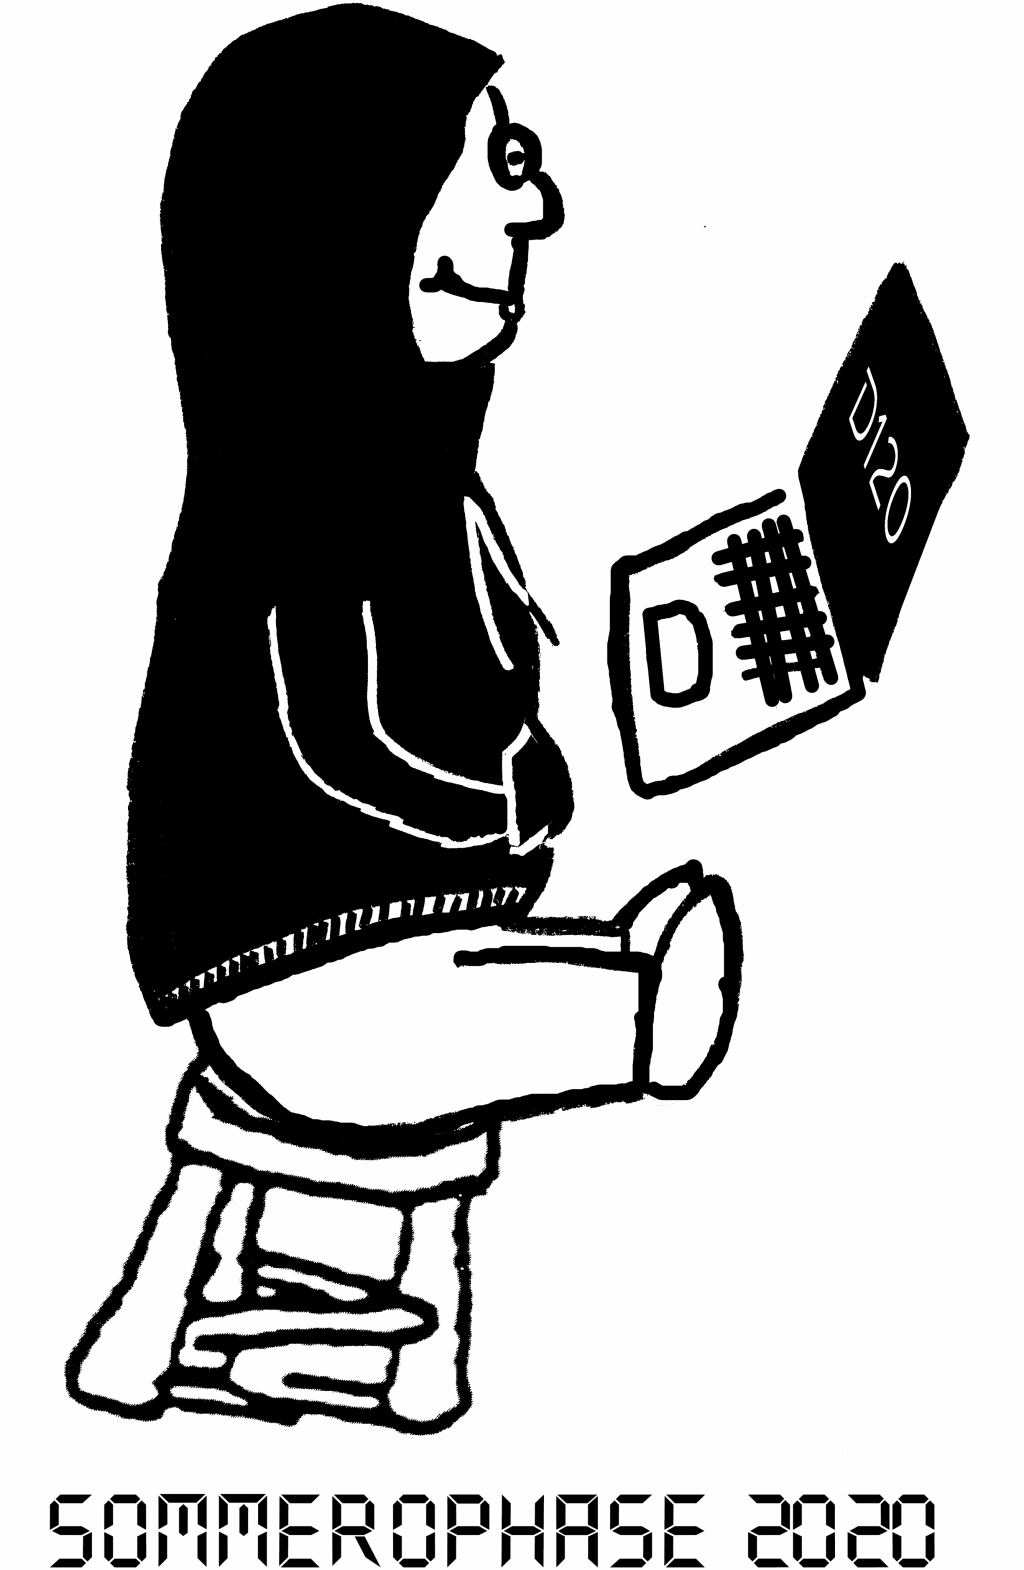
\includegraphics[width=2cm]{wesen/wesen_ophase}
%     \end{textblock*}

%     \begin{textblock*}{12cm}(1.5cm,1cm)
%         
\includegraphics[width=12cm]{inforz_schwarz}
%     \end{textblock*}

%     \definecolor{mycolor}{HTML}{C63313}  % diese Farben wurden willkürlich gewählt

%     \begin{textblock*}{12cm}(6.5cm,3.5cm)
%         \centering\fontsize{25}{25}\sffamily\textbf{
%             \textcolor{mycolor}{Master } \\
%             \textcolor{mycolor}{Deutsch}}
%     \end{textblock*}



%     \begin{textblock*}{12cm}(1.5cm,19cm)
%         %\centering\huge\sffamily\textbf{
%         %\textcolor{white}{Willkommen zur Ophase der Fachschaft} \\
%         %\textcolor{white}{Informatik im Sommersemester \the\year !}}
%     \end{textblock*}


%     \begin{textblock*}{7cm}(7cm,5cm)
%         \begin{flushright}
%             \large\sffamily\textbf{
%                 \textcolor{black}{Zeitschrift der Studierenden der}\\
%                 \textcolor{black}{Informatik der TU Darmstadt}}
%         \end{flushright}
%     \end{textblock*}

%     \begin{textblock*}{18cm}(1.5cm,8cm)
%         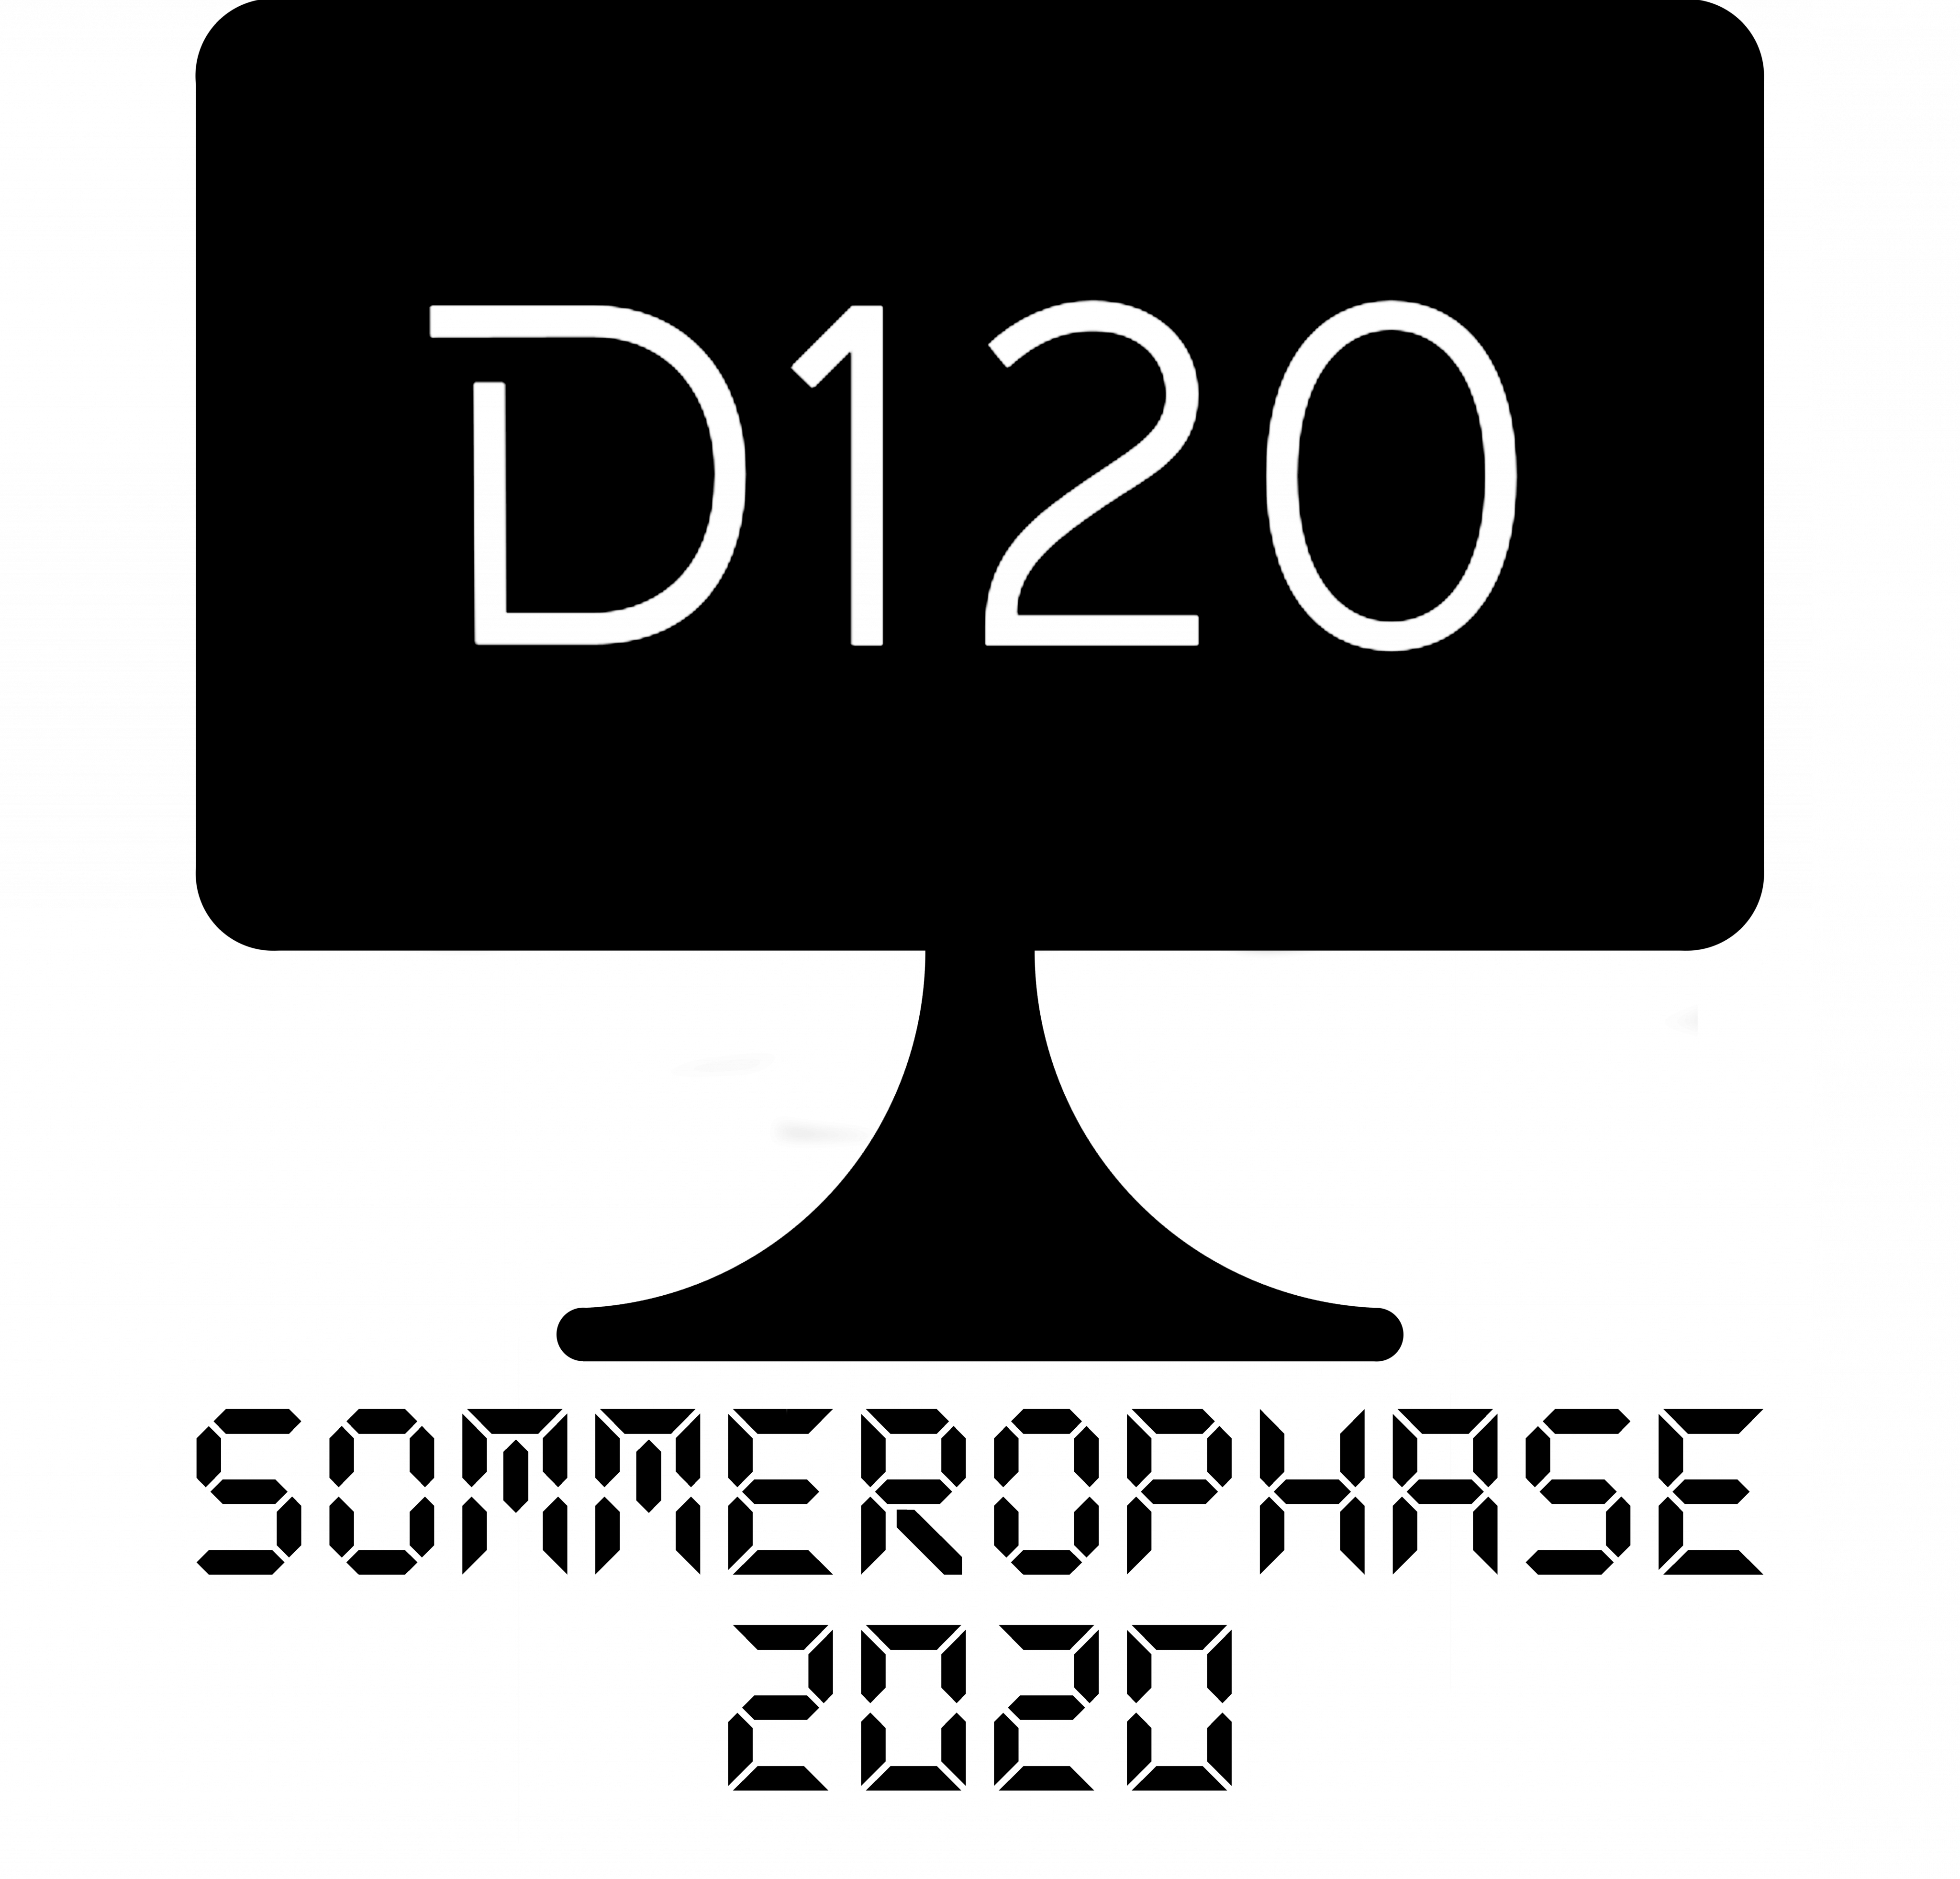
\includegraphics[width=12cm]{oinforz_cover_ss20}
%     \end{textblock*}

%     \begin{textblock*}{5cm}(1cm,9cm)
%         \begin{rotate}{90}
%             \sffamily\huge\textbf{
%                 \textcolor{black}{Inforz zur \ophase}}
%         \end{rotate}
%     \end{textblock*}


%     \begin{textblock*}{2cm}(1cm,14cm)
%         \begin{rotate}{90}
%             \sffamily\small \textcolor{black}{Preis: unbezahlbar}
%         \end{rotate}
%     \end{textblock*}


%     \begin{textblock*}{2cm}(1cm,20cm)
%         \begin{rotate}{90}
%             \sffamily \textcolor{black}{ISSN: 1614-4295}
%         \end{rotate}
%     \end{textblock*}

% \end{titlepage}
% \newpage


    % Stundenplan
    \thispagestyle{empty}
\vspace{5cm}

\begin{figure}
	\centering
	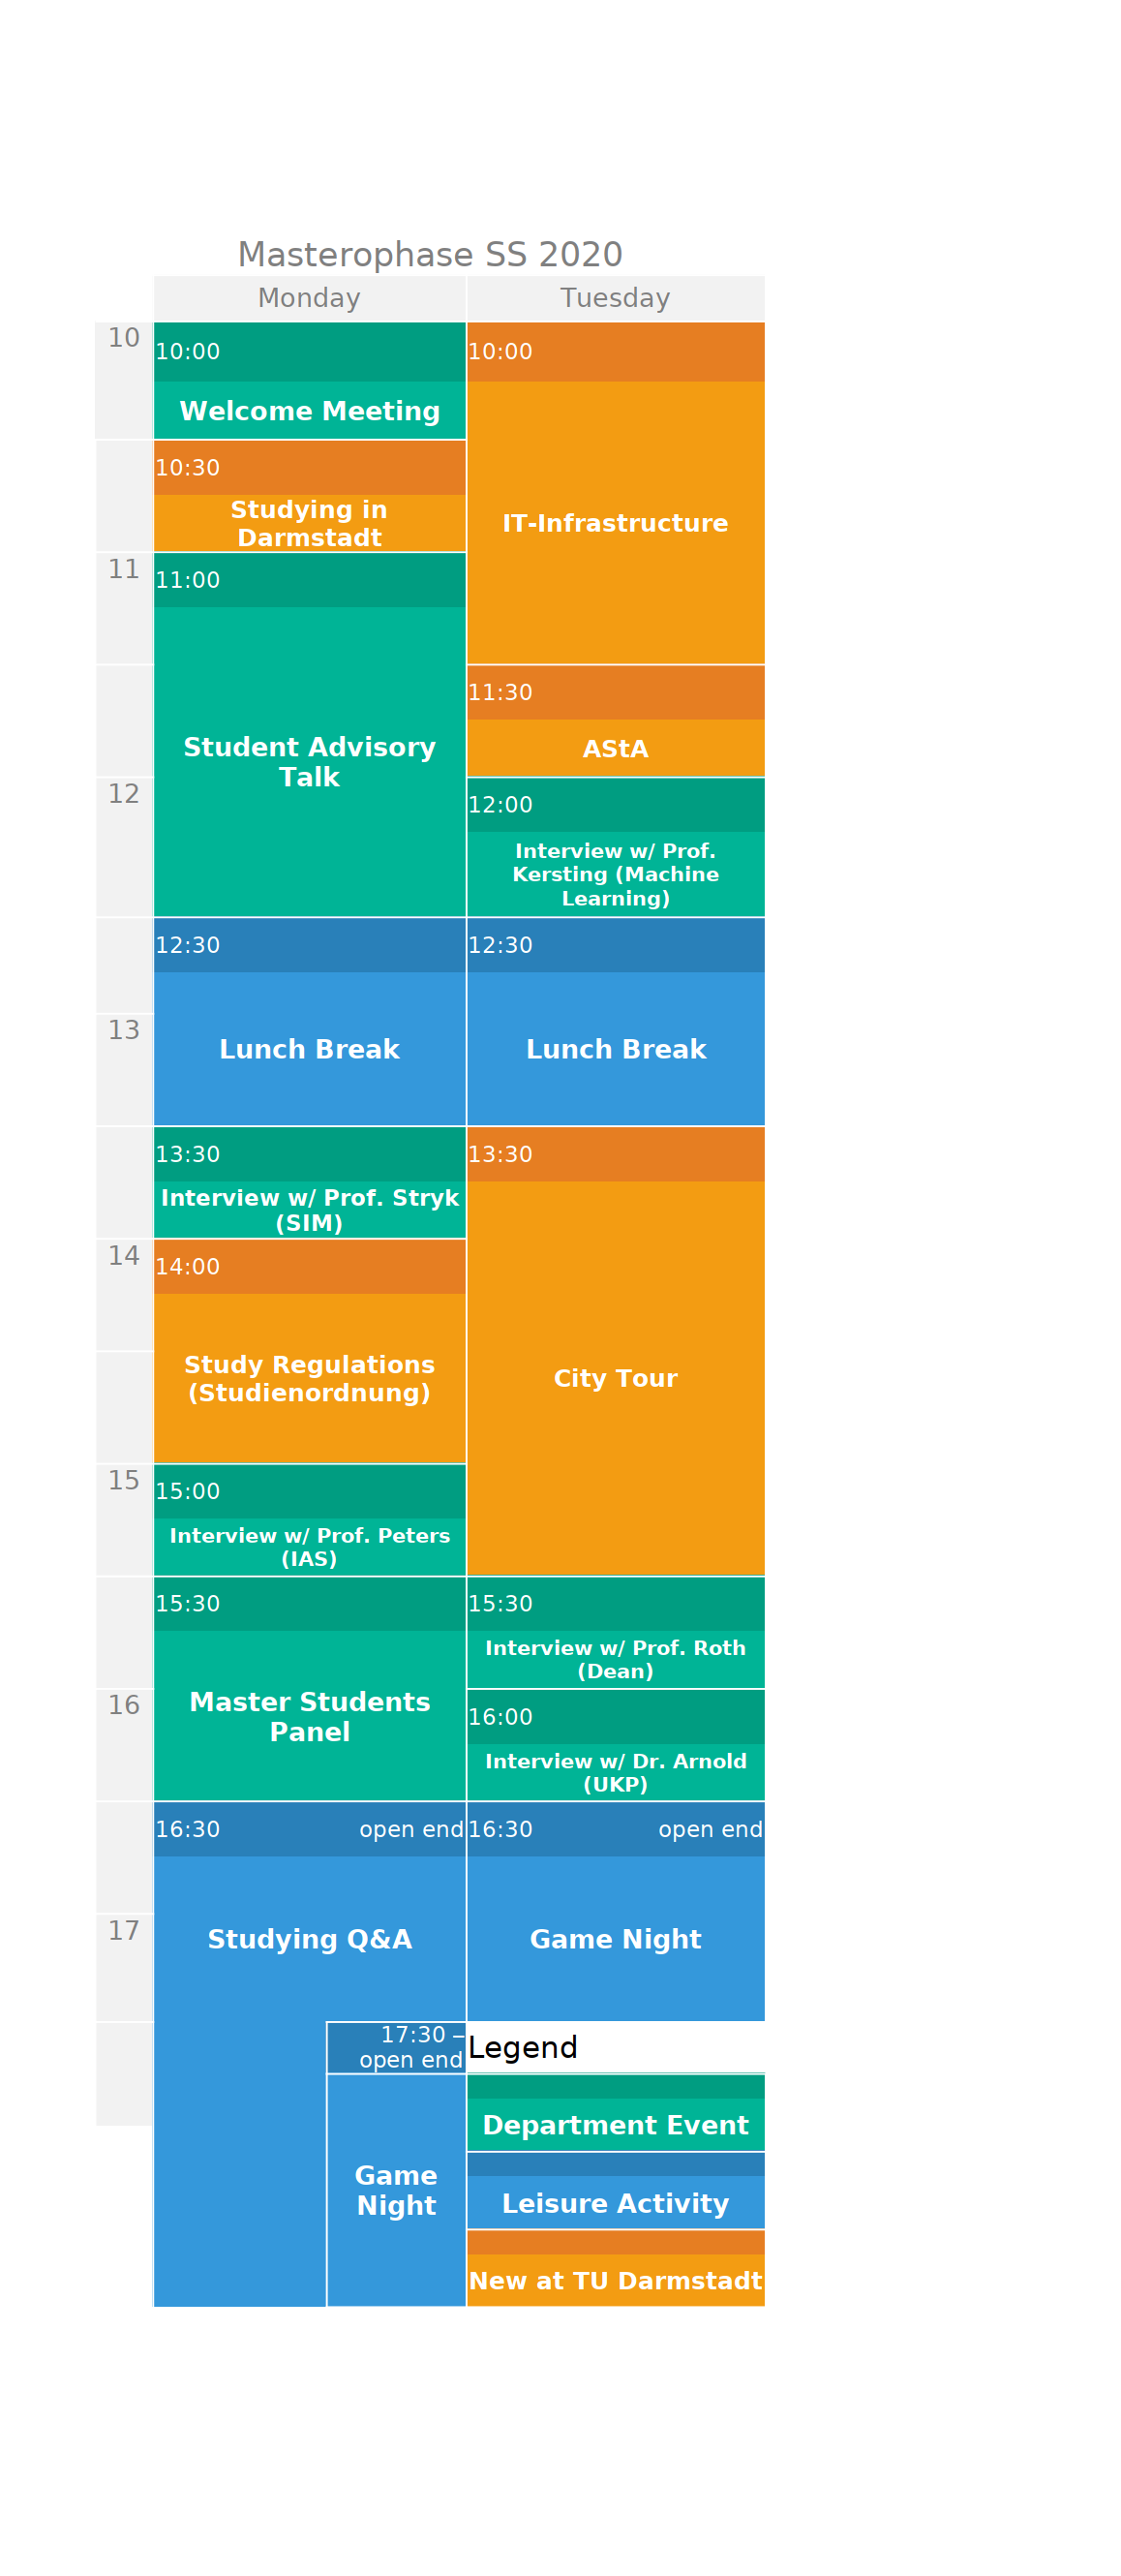
\includegraphics[angle=0,width=.8\linewidth]{../grafik/stundenplan_cyberphase_de}
	\caption{Stundenplan der Cyberphase}
\end{figure}

\cleardoublepage


    % Inhaltsverzeichnis
    \tableofcontents

    % Inhalt
    \kapitel{Willkommen}{../grafik/wesen/wesen_ophase}{}{}

\artikel{Vorwort des Dekanats}{Liebe Studierende,}{

    Herzlich willkommen am Fachbereich Informatik der TU Darmstadt!
    Sie haben eine sehr gute Wahl getroffen. Der Fachbereich Informatik ist einer der drei ältesten Informatik-Fachbereiche in Deutschland, gleichzeitig aber auch einer der modernsten. So haben wir als erster Fachbereich auf Bachelor- und Master-Studiengänge umgestellt und bieten Ihnen heute eine große Auswahl an spezialisierten Master-Studiengängen und Vertiefungsfächern an, die in dieser Form in Deutschland einzigartig ist. Doch Vielfalt ist nichts ohne Qualität. Diese wird durch die seit Jahren sehr hohe Einschätzung von Personalchefs zu den besten Informatik-Studiengängen in Deutschland belegt.


    %Die Leerzeichen sollen verhindern, dass LaTeX die Zeilenumbrüche zu lang zieht.
    \

    Der hervorragende Ruf kommt nicht von ungefähr. Das Studium der Informatik an der TU Darmstadt ist anspruchsvoll, auch wenn Ihnen das möglicherweise nicht sofort so vorkommen wird. Lassen Sie sich nicht täuschen. Anspruch und Tempo der Lehrveranstaltungen steigen danach schnell an. Nutzen Sie daher die ersten Wochen, um sich zu orientieren und gut in das neue Umfeld einzuleben. Die von der Fachschaft Informatik organisierte Orientierungsphase bietet dazu eine hervorragende Gelegenheit.

    \

    Insbesondere im Masterstudium an einer Universität sind Sie für Ihr Vorankommen selbst verantwortlich. Einer unserer ehemaligen Dekane hat den Unterschied von der Schule zur Universität mit den verschiedenen Arten von Wegen auf einem Berg verglichen. Die Schule ist ein Wanderweg auf einer Alm, der breit und gut beschildert ist. Auf dem Weg kommen Sie vielleicht manchmal in Atemnot und der Schweiß rinnt Ihnen in die Stirn, aber nachträglich können Sie sich vermutlich an wenige außerordentliche Schwierigkeiten mehr erinnern.

    \

    %\bildmitunterschrift{../grafik/willkommen/muehlhaeuser_sw}{width=35mm}{Prof.~Dr.~Max Mühlhäuser}{}

    An der Universität geht es dagegen darum, von der Alm auf den felsigen Gipfel zu klettern. Sie bietet dazu ein Gewirr von Kletterpfaden an, aus denen Sie sich einen auswählen und das Ziel, begleitet von Bergführern (Dozenten, Tutoren und Mentoren), erklimmen. Die Bergführer stellen Ihnen die notwendige Ausrüstung zur Verfügung. Sie werden Sie jedoch niemals hochziehen, sondern Ihnen nur die nächsten Griffe zeigen. Klettern müssen Sie selbst!

    \

    Sie werden sich jede Woche selbst motivieren müssen, um zu den Vorlesungs- und Übungsstunden zu gehen, die Übungsaufgaben zu bearbeiten und sich auf die Klausurprüfungen vorzubereiten. Dabei ist der Lehrstoff umfangreicher und anspruchsvoller zuvor, so dass die Bearbeitung eines einzelnen Übungsblattes leicht einen Tag oder mehr beanspruchen kann. Und eine gute Prüfungsvorbereitung erfordert Wochen sorgfältiger Planung und konsequenter Durchführung.

    Wenn Sie sich nun bei dieser Klettertour sorgen sollten, dass der derzeitige Klettersteig oder die verwendete Klettertechnik nicht zum Gipfel führen oder Ihre eigenen Kräfte übersteigen sollten, dann ist es Zeit, die Route mit den Bergführern im Detail zu studieren. Vielleicht wäre eine andere Route besser für Sie geeignet, vielleicht war ein Fehler in der Wegbeschreibung, vielleicht gab es ein Missverständnis bei der letzten Besprechung, vielleicht sollten Sie ein Trainingslager aufsuchen. Es kann viele Gründe geben, frustriert zu sein. Da hilft dann nur die Analyse: Wo stehe ich im Studium, wo will ich hin und wie kann ich meine Fähigkeiten bestmöglich einsetzen und weiterentwickeln, um dorthin zu kommen? Dabei lassen wir Sie nicht allein, sondern stehen bereit, Sie mit verschiedenen Angeboten zu unterstützen. Scheuen Sie sich daher nicht, sich an Ihre Professoren, Mentoren, Tutoren und Studienberater zu wenden, damit wir gemeinsam mit Ihnen Lösungen für etwaige Probleme erarbeiten können.

    \

    %\bildmitunterschrift{../grafik/willkommen/fischlin_studiendekan}{width=35mm}{Prof.~Dr.~Marc Fischlin}{}

    Vergessen Sie aber bei aller Anstrengung auch nicht, sich umzublicken und die Aussicht zu genießen. Ihr Studium soll für Sie interessant sein und Spaß machen. Gleichzeitig ist es der Beginn eines neuen Lebensabschnittes mit exzellenten Möglichkeiten, den eigenen Horizont enorm zu erweitern sowie neue Erfahrungen und neue Freundschaften fürs Leben zu gewinnen. Nutzen Sie die vielfältigen Möglichkeiten, um einen Ihren Interessen angepassten Weg zu finden! Bewegen Sie sich nicht immer auf ausgetretenen Trampelpfaden. Schweifen Sie gelegentlich auch einmal bewusst ab vom Klettersteig und pflücken ein paar Blumen, aber behalten Sie dabei Ihr Ziel im Auge.

    \

    Im Hinblick auf den Studienabschluss sollten Sie auch nicht vergessen, dass reine Spezialisten nur im Studium scheinbar erfolgreich sind und dass der spätere Erfolg beim Berufseinstieg und im Beruf nur zum Teil
    von fachlichen Fähigkeiten und guten Noten im Abschlusszeugnis bestimmt wird. Den anderen Teil des Erfolgs machen überfachliche Qualifikationen aus. Je nach künftiger Tätigkeit kann es mitentscheidend sein, ob man gut argumentieren und in Wort und Schrift überzeugend formulieren kann, ob man als Teamplayer und Teamleiter gleichermaßen befähigt ist, ob man mit Kritik gut umgehen kann oder manches andere mehr. Wir empfehlen Ihnen daher, diese wichtigen überfachlichen Qualifikationen im Studium bewusst weiter zu entwickeln.

    \

    Am besten stellen Sie sich dann zur Erreichung dieser Zwischenziele ein Portfolio zusammen aus speziellen Kursen, besonders förderlichen fachlichen Lehrveranstaltungen, Tutoren- oder Hilfsassistenten-Tätigkeiten und Selbststudien-Anteilen. Eine besonders erwähnenswerte Möglichkeit ist das Engagement in der Fachschaft, die nicht nur diese wichtige Orientierungsphase für Sie organisiert hat, sondern die sich auch in vielfältiger Weise wirksam und konstruktiv für die Belange der Studierenden einsetzt und damit wertvolle und wichtige Beiträge zur Entwicklung des Fachbereichs Informatik leistet. So werden Sie vom Konsumenten zum Mitgestalter des Informatikstudiums in Darmstadt.

    \

    Nun wünschen wir Ihnen einen guten Start in das Informatikstudium an der TU Darmstadt!
}
{Prof.~Stefan Roth, Ph.D.~(Dekan) \\Prof. Dr. rer. nat.~Michael Waidner (Studiendekan)}

\newpage


\artikel{Willkommen an der Universität}
{Die Fachschaft Informatik heißt Dich zu Deinem Studienbeginn herzlich willkommen.}{
    Du wirst es voraussichtlich schon an mehreren Stellen gelesen und gehört haben und auch an dieser Stelle wird es Dir nicht erspart: Herzlich willkommen im Master-Studium, willkommen an der Technischen Universität Darmstadt, willkommen zum Beginn eines neuen Lebensabschnittes!

    Einiges dürfte ähnlich wie an Deiner alten Uni ablaufen, vieles aber auch anders. An der TU Darmstadt, und insbesondere am Fachbereich Informatik, stehen Dir jede Menge Möglichkeiten offen, Hilfe bei allen Deinen Fragen und Problemen zu bekommen, zum Beispiel die Ophase, in der Du erfahren kannst, wie Du Dein Studium sinnvoll gestalten kannst. Und natürlich auch wir – die Fachschaft Informatik – immer für Dich da und versuchen, Dir mit Rat und Tat zur Seite zu stehen.

    Wir wünschen Dir, dass Du auch während Deines Studiums jede Menge Freundinnen und Freunde findest, die mit der gleichen Motivation studieren wie Du und mit denen Du gut auskommst. Und versuche, daran zu denken, dass das Studium aus mehr besteht als nur Lernen: es ist ein Lebensabschnitt, den Du auch genießen solltest – und dafür wünschen wir Dir nur das Beste.
}
{Die Fachschaft Informatik}

\vfill

\noindent
\bildmitunterschrift{willkommen/fsbild}{width=\textwidth}{Einige Mitglieder der aktiven Fachschaft im Wintersemester 2019/2020}{Bild von Tim Pollandt und Stefanie Blümer}

\newpage

\artikel{Willkommen zur Ophase}
{Wenn Du dieses Heft in der Hand hältst und diesen Artikel liest, dann stehen die Chancen gut, dass Deine Orientierungsphase gerade begonnen hat oder Du bereits mitten drin bist.}
{
Die Ophase am Fachbereich Informatik ist eine Veranstaltung mit langer Geschichte: In etwa seit es den Fachbereich Informatik gibt, gibt es auch eine Orientierungsphase für Erstsemester. Der Sinn dieser Veranstaltung ist es, Dir die Universität, und insbesondere den Fachbereich Informatik, näher zu bringen, Dich mit Deinen Kommilitoninnen und Kommilitonen, also denjenigen Leuten, mit denen zusammen Du Dein Studium bestreiten wirst, bekannt zu machen und Dir einen guten Start ins Studium zu ermöglichen.

All das, was Dir diese Woche geboten wird, ist von Studierenden organisiert und durchgeführt, um Studienanfängerinnen und \\ -anfängern wie Dir einen optimalen Start ins Studium zu ermöglichen. Die Organisator*innen, die Dich diese Woche betreuen, sind Studierende, die, genau wie Du jetzt, auch einmal eine Ophase mitgemacht haben und sich ein paar Semester später dazu entschlossen haben, das, was sie damals gelernt haben, an neue Studierende wie Dich weiterzugeben.

Auch dieses Ophasen-Inforz, eine Sonderausgabe der Fachschaftszeitung Inforz, ist Teil der Ophase und beinhaltet alle Informationen, die Du im Laufe dieser Woche vermittelt bekommst – und noch viele mehr. Dennoch ist es natürlich empfehlenswert, die Veranstaltungen, die in der Ophase angeboten werden, insbesondere die Kleingruppen und den Vortrag zur Studienorganisation zu besuchen. Dort hast Du nämlich, im Gegensatz zum reinen Lesen dieses Heftes, die Möglichkeit, Fragen zu allen wichtigen Themen rund um Universität und Studium zu stellen und natürlich auch, mit anderen Studierenden in Kontakt zu kommen. Für Letzteres gibt es auch noch zusätzliche Freizeitangebote in der Ophase, wie Kneipentouren, welche im kommentierten Stundenplan (ein paar Seiten weiter) genauer erklärt sind.
Wir wünschen Dir noch viel Spaß mit diesem Heft und eine gelungene Ophase!
}
{Die OInforz-Redaktion}
\vfill
\bildmitunterschrift{../grafik/comics/cautionary}{width=\textwidth}{}{xkcd.org}
\newpage

\artikel{Kommentierter Stundenplan}
{Auf dem Innenumschlag dieses Inforz findest Du Deinen Stundenplan für die erste Woche. Hier wollen wir etwas näher darauf eingehen, welche Veranstaltungen für wen gedacht sind.}
{\textbf{Plenumsveranstaltung}

    Am Montag beginnt die Cyber-O-Phase um 10 Uhr morgens, mit einer Begrüßung durch den Fachbereich. Dabei wird auch darauf eingegangen, welche Inhalte die O-Phasen-Veranstaltungen behandeln. Des Weiteren sind über die Tage von Montag und Dienstag viele Interviews von Professoren über eure Studienbereiche für euch geplant, bei denen ihr live Fragen stellen könnt.  Außerdem haben wir am Montagnachmittag ab 16 Uhr ein Studien Q\&A geplant, bei welchem ihr euren Studienvorreitern Fragen zu ihrem, bzw. nun auch eurem, Studium stellen könnt. \\

    \textbf{Stadtführung}
    Für alle, die sich in Darmstadt noch nicht so gut auskennen, laufen wir am Dienstag ab 14 Uhr mit einer Kamera einige wichtige Orte in Darmstadt ab und erklären euch ein bisschen was dazu, natürlich könnt ihr die Informationen auch später noch zu jeder Zeit nachgucken.\\

    \textbf{Spaß und Freizeit}
    Da dieses Semester alles digital sein wird, bieten wir Montagabend ab 17 Uhr und Dienstagabend ab 16 Uhr eine Game-Night mit zum Beispiel Minecraft, Counter-Strike, usw. an. Während ihr hier zusammen zockt könnt ihr euch gleichzeitig auf Discord besser kennenlernen und schon einmal erste nähere Kontakte zu euren neuen Studienkollegen knüpfen.
}{}

\vfill
\bildmitunterschrift{../grafik/comics/self_description}{width=\textwidth}{}{xkcd.org}
%\artikel{Workshops}{Hier finden ihr mehr Informationen über die einzelnen Workshops}{

    \textbf{Jonglieren mit drei Bällen}\\
    In diesem Workshop lernen wir das Jonglieren mit drei Bällen, genauer gesagt das Grundmuster: Die 3-Ball-Kaskade.
    Dies geschieht von Grund auf, wir beginnen mit einem Ball und arbeiten uns dann hoch. Am Ende sollte jeder Teilnehmer die Grundlagen beherrschen
    und in der Lage sein, selbst weiter zu üben. Wer besonders schnell ist, kann auch schon einfachere Tricks ausprobieren oder sogar Vorübungen zu vier Bällen lernen.
    Jonglieren selbst kann als Partytrick, zur Verbesserung von Konzentrationsfähigkeit und dem räumlichen Denkvermögen oder gar als neues Hobby dienen. Ich freue mich auf euch!
    \autor{Nathanael Herwig}

    \textbf{Esperanto}\\
    "Saluton, kara leganto!"
    Am Schreibtisch entworfen, gibt es die Sprache Esperanto seit knapp 130 Jahren. Und doch: Sie lebt und das Konzept einer neutralen Kommunikation auf Augenhöhe begeistert Menschen weltweit. Auch wenn sie heute vorwiegend im kleinen Maßstab angewendet wird, lohnt es sich dieses verbindende Kulturgut zu pflegen. Die klaren Strukturen machen Spaß und bieten einen sanften Einstieg in die Welt der Sprachen. Neben der Einführung in die Grammatik, erwartet euch in diesem Workshop auch ein kleiner Abstecher in die bemerkenswerte Geschichte.
    \autor{Sebastian Bremser}

    \textbf{Mesh-Netzwerke selber bauen}\\
    "Mesh" ist in den letzten Jahren eines der Top-Themen in den Marketingbroschüren und Datenblättern der Routerhersteller geworden. Freifunk ist einer der Pioniere auf dem Gebiet der Entwicklung und dem Aufbau von Mesh-Netzwerken. In diesem Workshop lernst du, wie du dein eigenes, privates Mesh-Netzwerk aufbaust, indem du mit deinen Kommilitonen ein hybrides und verschlüsseltes Mesh-Netzwerk von Grund auf aufbaust.
    \autor{Freifunk Darmstadt}

    \textbf{Blick unter die Haube - PC (de-)montieren und Linux installieren}\\
    Aus welchen Teilen besteht ein PC und wozu sind diese da?

    Im Workshop werden wir in einem kurzen Vortrag die einzelnen Teile eines PCs erläutern. Hands-On wird es Anschauungsobjekte wie geöffnete Festplatten (HDD und SSD), Grafikkarten, CPUs usw. geben.
    Im Anschluss erhalten alle Teilnehmer*innen einen Desktop-PC bei dem Sie RAM und Festplatte  ersetzen und im Anschluss auf dem PC Linux installieren.
    \autor{Stephan Voeth}

    \textbf{Latex}\\
    Hast du schonmal versucht in Office eine richtig komplizierte Formel einzugeben?
    Oder ein Dokument mit vielen Seiten und Bildern genau so zu formatieren, wie eine
    Vorgabe vorgibt? Und plötzlich fällt dir auf, dass du einen Fehler gemacht hast
    und du jetzt bei 50 Überschriften die Schriftgröße anpassen musst? Und am Ende sieht
    plötzlich alles wieder ganz anders aus, sobald du irgendwo eine Zeile änderst oder
    das ganze auf einem anderen Computer öffnest. Zum Glück gibt es etwas, womit das
    viel einfacher geht: LaTeX. Und trotz des komischen Namens wird es auf der ganzen
    Welt von fast allen Wissenschaftlern und von vielen Anderen eingesetzt, wenn sie
    technische oder mathematische Dokumente erstellen. LaTeX ist ein bisschen wie HTML
    und CSS, man schreibt einen reinen Text, versieht ihn mit Markierungen, welcher
    Block welche Rolle hat und kann ihn dann mit speziellen Programmen in formatierte
    Dokumente übersetzen. Klingt nützlich? Ist es auch. Und je eher man anfängt, es zu
    nutzen, desto mehr Ärger kann man sich ersparen. Deshalb bieten wir in diesem Workshop
    einen einfachen und kurzen Einblick. Und irgendwann im Laufe des Studiums braucht
    es sowieso (fast) jeder. Warum also nicht gleich?!


    \textbf{Capture The Flag: Hacking als Wettkampf}\\
    Capture The Flag, oder kurz CTF, sind IT-Security Wettkämpfe über einen begrenzten Zeitraum, bei denen um die Wette gehackt wird.
    Dabei gilt es Aufgaben zu lösen und dadurch Punkte zu gewinnen. Am Ende gewinnt das Team mit den meisten Punkten.

    Die Aufgaben kommen hierbei aus den Bereichen Reverse Engineering, Web Security, Binary Exploitation, Forensik, Kryptographie, Mobile Security und ähnlichem und sind sehr praxisorientiert.

    Wir, das CTF-Team des Darmstädter Chaos Computer Club, wollen euch in diesem Workshop eine hands-on Einführung in dieses Format geben und euch bei euren ersten Flags zur Seite stehen und Fragen beantworten und Hilfestellung geben.
    \autor{Alexander Druffel}

    \textbf{Programmierung von Lego Mindstorms Robotern}\\
    Du hast schon mal ein paar Programmzeilen getippt und willst mal ein bisschen spielerisch testen, ob der Code auch das macht was du willst?
    Hier kannst du einem Lego Mindstorms Roboter programmieren und schon mit wenig Code kleine Aufgaben lösen.
    \autor{David Botschek}

    \textbf{Einstieg in die Entwicklung von Webanwendungen}\\
    Ich möchte den Teilnehmern einen Einblick in die Webentwicklung geben. Dabei gehe ich zuerst auf HTML, Javascript und ein wenig CSS ein und werde dann noch darüber sprechen, wie die Entwicklung mit Framworks und Libraries aussieht. Ziel ist es den Teilnehmern einen groben Überblick über Sprache, Tooling uns sonstiges zu vermitteln.
    \autor{Nicklas Knell}

    \textbf{Studium für Späteinsteiger}\\
    Ich biete einen kleinen Vortrag zum Thema und anschließend einen Workshop für alle, die ein bisschen später zum Studium gefunden haben.
    \autor{Malin Kammer}

    \textbf{Musiknotation und Arrangieren - Einführung in Open-Source-Musiknotation mit MuseScore}\\
    Noten schreiben leicht gemacht! Dieser Workshop richtet sich an alle Studierenden, die Musik schreiben, komponieren, arrangieren oder einfach mal in die Welt der meistgenutzten Open-Source-Musiknotationssoftware MuseScore reinschnuppern wollen. Nach einer kurzen Einführung in das Programm werden wir uns mittels Try-and-Error der Umsetzung Eurer Ideen widmen - Ausprobieren, Arrangieren, Komponieren. Gerne gibt es "Tipps und Tricks der Harmonielehre", den "Unterschied zwischen Tremolo und Triller" oder einen "Crashkurs Bassschlüssel" oben drauf.

    Der Workshop ist auch für Anfänger ausgelegt, es sind keine Vorkenntnisse in der Benutzung von MuseScore nötig. Allerdings solltest du Interesse an Musik haben, rudimentär Noten lesen können und bei dem Wort Andante nicht unbedingt an Nudeln beim Italiener denken.

    Und weil alles mit einem Zitat seriöser wirkt... "Der Takt ist nicht das Zählwerk, sondern der Puls der Musik." (Ulrich Erckenbrecht)
    \autor{Jannis Rösner}

    \textbf{Flaschen-Yoga}\\
    Mehr Bewegung für Informatiker! Wir machen mit euch Yoga für Anfänger - nur anders: Beim Flaschen-Yoga halten wir bei diversen Grundübungen eine offene Flasche in der Hand, die weder abgestellt noch verschüttet werden darf. Austrinken ist jedoch erlaubt. Es macht auf jeden Fall Spaß!
    \autor{Yvonne Meuleneers und Viola Hofmeister}



    \textbf{Einführung in die Hochschulpolitik}\\
    Einführung in die Hochschulpolitik (HoPo 101)

    In einem 10 Minütigen Vortrag kann man nicht vollumfänglich
    über die Hochschulpolitik an der TU Darmstadt aufklären.
    Daher wird dieser Workshop angeboten.

    Ziel ist es die Möglichkeiten studentischer Beteiligung
    sowohl an der Uni (Universitätsversammlung, Senat,...),
    als auch in der studentischen Selbstverwaltung
    (Studierendenparlament, AStA) zu betrachten.
    Damit sollen die Teilnehmenden die Möglichkeit erhalten
    die Politik der Studentischen Gremienmitglieder kritisch
    bewerten zu können oder sogar sofern gewünscht sich
    selbst zu beteiligen.

    Die Workshopleitung ist selbst in der Darmstädter Hochschulpolitik
    aktiv, werden sich jedoch alle Mühe geben, ihre persönliche Meinung
    entssprechend zu kennzeichnen und von Faktenbeschreibungen zu
    trennen.
    \autor{Tobias Huber}

    \textbf{Rugby - Ein Sport für jeden}\\
    Hallo, wir von der Unisportgruppe Rugby wollen euch herzlich an der TU Darmstadt begrüßen und euch unseren Sport näherbringen.
    Dazu laden wir euch in der Herrngarten ein. Dort haben wir für euch ein kleines Programm vorbereitet, das Rugby in jedem Bereich gerecht wird. Unser Sport richtet sich an alle - und damit meinen wir alle. Deswegen kommt vorbei, wir freuen uns auf euch
    \autor{Christoph Schülter}

    \textbf{Codestyle? Warum, läuft doch!}\\
    Tabs oder Spaces, Klammern mit und ohne Leerzeichen, geschweifte Klammern auf der selben oder in der nächsten Zeile: Es gibt sehr viele verschiedene Arten, Code zu formatieren - leider oft auch mehrere verschiedene Formatierungsarten in einem Projekt oder sogar in derselben Datei. Dadurch können sich Bugs besser verstecken und die Zusammenarbeit im Team wird durch unlesbaren Code erschwert.

    Wir zeigen euch, wie ihr euch im Team auf einen gemeinsamen Programmierstil einigen könnt und welche Tools euch dabei helfen, diesen durchzusetzen. So wird das Bearbeiten von komplexen Programmierpraktika für euch leichter und euer Code für die Tutoren besser verständlich.

    Guten Code zeichnet mehr aus, als fehlerfrei und kompakt zu sein. Code muss sich selbst dokumentieren und wartbar sein. Nur dann ist eine gemeinsame Entwicklung in Projekten möglich.
    \autor{Pickware GmbH}

    \textbf{Stundenplanerstellung und Informations-/ Fragerunde für alle "Nicht-Bachelor of Science-Studiengänge"}\\
    Dieser Workshop soll eine Möglichkeit bieten, den Student*innen, welche nicht im Bachelor of Science studieren, offengebliebene Fragen zu beantworten, beim Erstellen der Stundenpläne zu helfen, generelle Hilfestellungen zu geben, oder sich unter den Hunderten von Ersties auch einfach mal zu sehen und zu wissen, dass es noch andere mit dem selben Studiengang gibt.
    \autor{Dini \& Guido (vermutlich auch ein Assitent von Hr. Gallenbacher)}
}{}



    \kapitel{Studium}{../grafik/wesen/wesen_tafel}
{Universität: ein Ort, wo Kieselsteine geschliffen und Diamanten getrübt werden.}
{Robert Green Ingersoll, 1833 - 1899, US-amerikanischer Redner}

\artikel{Das Wesen der Informatik...}{
    ...ist seit vielen Jahren das Maskottchen der Fachschaft Informatik. Es ist ein kleines Baby, das mit einem unschuldigen Grinsen auf einem Hocker sitzt -- mit einem Sturmgewehr in der Hand. Da kommt bei manchen wohl gleich der Gedanke an die \glqq bösen Killerspiele\grqq.  Doch weit gefehlt: Das symbolische Wesen der Informatik fand sich zum ersten Mal im Jahr 1986 auf der Zeitschrift Inforz, also zu einer Zeit, als der Begriff des Ego-Shooters noch gar nicht existierte.}
{Die Intention damals war eine andere: Was passiert, wenn man einem Baby eine Schusswaffe in die Hand drückt? Keiner weiß es genau, aber jeder hat ein ungutes Gefühl dabei.
    Die Informatik ist jung, vor allem im Vergleich zu anderen Wissenschaften. Physik, Mathematik, Biologie und Philosophie sind seit mehreren hundert bis tausenden von Jahren als eigenständige Disziplinen anerkannt.  Im Gegensatz dazu existiert allein der Begriff der \glqq Informatik\grqq~erst seit Mitte des 20. Jahrhunderts und als eigenständige wissenschaftliche Disziplin wurde sie erst in den späten 1960er-Jahren etabliert.
    Wer konnte also 1986, gerade mal etwas über ein Jahrzehnt nach der Entstehung des Fachbereichs Informatik an deutschen Universitäten, schon die Konsequenzen abschätzen, die diese neue Wissenschaft mit sich bringen würde?\\

    \textbf{Was ist Informatik?}

    Laut Wikipedia ist die Informatik die \glqq Wissenschaft der systematischen Verarbeitung von Informationen, insbesondere der automatischen Verarbeitung mit Hilfe von Digitalrechnern\grqq.
    Das klingt erstmal nicht besonders spannend oder gefährlich. Das Ganze dient dazu, Probleme einfacher und effizienter  zu lösen als es bisher möglich war - und das so automatisiert wie möglich. Einfach, effizient, automatisiert - das sind schon ganz nette Eigenschaften, die einem Menschen das Leben leichter machen können. Da kann doch eigentlich nichts schiefgehen.\\

    \columnbreak

    \textbf{Beispiel: Wegfindung}

    Eines der bekanntesten und ältesten Probleme in der Informatik ist die Wegfindung. Ziel ist es, von einem Startpunkt A möglichst günstig zum Ziel B zu gelangen. \glqq Möglichst günstig\grqq kann in diesem Fall einiges sein: kürzester Weg, schnellster Weg, Weg mit den angenehmsten Bedingungen oder auch Weg mit den meisten Sehenswürdigkeiten auf der Strecke. Eine Anwendung sind ganz offensichtlich Navigationssysteme für Autos oder andere Transportmittel wie Schiffe und Flugzeuge, um dem Menschen, der diese Geräte steuert, Zeit- und Geldeinsparungen zu ermöglichen. Aber auch schwer bewaffnete Kampfdrohnen verlassen sich auf Wegfindungsalgorithmen, um einfach, effizient und automatisiert gesuchte Terroristen oder andere unliebsame Personen liquidieren zu können.\\

    \bildmitunterschrift{../grafik/wesen/wesen_transparent}{width=\columnwidth}{}{}

    \textbf{Ein 2. Beispiel: Roboter}

    Roboter werden schon sehr lange in der Industrie eingesetz, um Tätigkeiten zu übernehmen, die für Menschen zu schwer oder gefährlich sind. Die Automobilindustrie ist hier ein gutes Beispiel. Stationäre Roboterarme wuchten hier schwere Teile durch die Gegend, setzen sie zusammen und überprüfen bisweilen auch schon in Zusammenarbeit mit vernetzten Sensoren verschiedene Qualitätseigenschaften der resultierenden Werkstücke. Der Mensch verkommt in diesen zunehmend digitalisierten Arbeitsumgebungen beisweilen sogar schon eher zum Störfaktor, denn dessen manuelle Arbeit ist bei weitem nicht so effizient wie die, die von Automaten verrichtetet wird. Mal ganz davon abgesehen, dass Menschen im Gegensatz zu Robotern ungünstigerweise auch noch schlafen müssen und trotzdem noch für ihre Arbeit Geld verlangen...\\

    \textbf{Noch ein Beispiel: Machine Learning und KI}

    Mit steigendem Rechen- und Speichervermögen von Computern bieten sich der Wissenschaft umfangreichere Möglichkeiten zur Datenauswertung als jemals zuvor. Dank künstlicher Intelligenz und maschinellen Lernverfahren können heutzutage Terabytes an Daten, wie sie beispielsweise in den Sensoren von Partikelbeschleunigern auftreten, innerhalb kurzer Zeit ausgewertet werden und ermöglichen somit ganz neue Forschungsfelder, zum Beispiel eben in der Partikelphysik, oder auch in der Hirnforschung. Aber nicht nur in den Laboren der Wissenschaft fallen große Datenmengen an. Spätestens seit Verbreitung des Internets befüllen auch Staaten und Dienstleistungsunternehmen beständig wachsende Datensammlungen, die mittels Lernalgorithmen auf Zusammenhänge untersucht werden. Das kann Menschen, die diese Dienste nutzen, das Leben sehr einfach machen, da Computer auf diese Weise immer besser verstehen lernen, worauf es einzelnen Nutzern ankommt -- zugleich versuchen jedoch die hinter diesen Diensten stehenden Unternehmen oder Staaten zunehmend, dieses Wissen um die individuellen Vorlieben gewinnbringend zu nutzen. Denn je besser man seine Kunden (oder Bürger) kennt, desto einfacher wird es, diese mit minimalem Aufwand und ohne menschliches Zutun zu manipulieren.\\

    \textbf{Informatik und Gesellschaft}

    Im Laufe von nur wenigen Jahrzehnten hat es die Informatik vollbracht, nahezu in jeden Bereich der Gesellschaft vorzudringen. Anhand der obigen Beispiele (und man könnte noch viele, viele mehr nennen) soll verdeutlicht werden, wie groß der Einfluss der Informatik auf unseren Alltag mittlerweile ist. In vielen Fällen handelt es sich um Errungenschaften, die unser Leben angenehmer machen und erleichtern, aber oftmals kommen diese mit Kosten, die wir bisweilen nicht direkt einsehen oder abschätzen können -- auch als Informatiker*innen nicht. Wir sind also vielmals sprichwörtlich die unbedarften Kinder, die mit der Schusswaffe spielen, wenn wir maßgeblich zu einer neuen technologischen Errungenschaft beitragen. Vielfach tendieren wir nämlich dazu, nur die wünschenswerten Einsatzzwecke in Betracht zu ziehen und den Schaden zu übersehen, der gleichzeitig mit der Technologie in useren Händen angerichtet werden kann. Die Informatik ist also weit mehr als nur eine (Ingenieurs-)Wissenschaft, denn letztendlich werden insbesondere wir Informatiker*innen diejenigen sein, die zukünftig die Richtung vorgeben, in die sich unsere Gesellschaft bewegt -- eine große Chance, aber auch eine große Bürde und eine Tatsache, die uns immer bewusst sein sollte.}
{Tobias Otterbein, Stefan Gries}
\newpage

%\addsec{Deine Dozent*innen im ersten Semester}

\textbf{Es schadet aber nicht, schon im Vorhinein zu wissen, wer der oder die jeweilige Dozent*in ist und wie man ihn oder sie erreichen kann, deshalb findest du hier eine Auflistung der Dozent*innen, die die Erstsemester-Veranstaltungen halten. Einige davon werden dir vielleicht auch schon in der Ophase begegnen.}\\

Im ersten Semester wirst du die Vorlesungen \textit{Funktionale und Objektorientierte Programmierkonzepte} (\textit{FOP}), \textit{Digitaltechnik} (\textit{DT}), \textit{Automaten, Formale Sprachen und Entscheidbarkeit} (\textit{AFE}) und \textit{Mathematik 1 für Informatik und Wirtschaftsinformatik} hören, sofern du die in der Ordnung des Studiengangs (siehe Artikel "`Die Ordnung des Studiengangs"') vorgeschlagenen Veranstaltungen besuchst.

Im Folgenden ist aufgeführt, wer diese Lehrveranstaltungen in diesem Semester halten wird und wie bzw. wo man diese Personen erreichen kann. Alle bieten offene Sprechstunden an. Wann diese stattfinden, erfährst du zu Beginn der jeweiligen Veranstaltung.

%\vspace{8mm}
\begin{tabular}{lc}

                                                                   &                   \\
    \textbf{Funktionale und Objektorientierte Programmierkonzepte}
    & \multirow{4}{*}{} \\
                                                                   &                   \\
    \textbf{Name:} Prof. Dr. Karsten Weihe                         &                   \\
    \textbf{Gebäude/Raum:} S2$|$02 E122                            &                   \\
    \textbf{E-Mail-Adresse:} weihe@informatik.tu-darmstadt.de      &                   \\
    \textbf{Zugehörigkeit:} Fachgebiet Algorithmik                 &                   \\

                                                                   & \\&               \\
    \textbf{Automaten, Formale Sprachen und Entscheidbarkeit}
    & \multirow{4}{*}{} \\
                                                                   &                   \\
    \textbf{Name:} Prof. Dr. Kord Eickmeyer                        &                   \\
    \textbf{Gebäude/Raum:} S2$|$15 204                             &                   \\
    \textbf{E-Mail-Adresse:} eickmeyer@mathematik.tu-darmstadt.de  &                   \\
    \textbf{Zugehörigkeit:} Arbeitsgruppe Logik                    &                   \\
                                                                   &                   \\

                                                                   & \\&               \\
    \textbf{Digitaltechnik}
    & \multirow{4}{*}{} \\
                                                                   &                   \\
    \textbf{Name:} Prof. Dr. Thomas Schneider                      &                   \\
    \textbf{Gebäude/Raum:} S4$|$14 5.3.14                          &                   \\
    \textbf{E-Mail-Adresse:} schneider@encrypto.cs.tu-darmstadt.de &                   \\
    \textbf{Zugehörigkeit:} Fachgebiet ENCRYPTO                    &                   \\
                                                                   &                   \\

                                                                   & \\&               \\
    \textbf{Mathematik I für Informatik und Wirtschaftsinformatik}
    & \multirow{4}{*}{} \\
                                                                   &                   \\
    \textbf{Name:} Prof. Dr. Thomas Streicher                      &                   \\
    \textbf{Gebäude/Raum:} S2$|$15 208                             &                   \\
    \textbf{E-Mail-Adresse:} streicher@mathematik.tu-darmstadt.de  &                   \\
    \textbf{Zugehörigkeit:} Arbeitsgruppe Logik                    &                   \\
\end{tabular}

\newpage

%
\artikel{Lehr- und Lernformen}
{Im Gegensatz zur Schule unterscheiden sich die Lehrformen an der Uni erheblich. In diesem Artikel stellen wir die an einer Universität üblichen Lehr- und Lernformen vor.
}{
    In großen Studiengängen herrscht über\-wiegend Massenbetrieb, so dass keine Kontrolle stattfindet. Die Verantwortung zum Lernen ist jedem selbst überlassen. Zum anderen sind die Anforderungen bezüglich der Lehrinhalte höher als in der Schule. Deshalb möchten wir dir die gebräuchlichsten Lehrformen an der Uni vorstellen. Es ist schließlich wichtig, sich über den eigenen Lernstil bewusst zu werden. Auch hierbei möchten wir ein paar gängige Methoden umreißen.

    Allgemein spricht man von einer Veranstaltung als Summe aller ihrer Teile. Eine Veranstaltung kann zum Beispiel nur aus einer Vorlesung bestehen, aus einer Vorlesung und einer Übung oder aus einer Vorlesung, einer Übung und einem Praktikum.
}{}

\noindent\textbf{Vorlesung}
\begin{multicols}{2}
    \bildmitunterschrift{../grafik/artikel/lul_vorlesung}{width=\linewidth}{}{}
    \begin{itemize}
        \item Gebräuchlichste Form am Fachbereich Informatik.
        \item Ein*e Dozent*in steht vorne im Hörsaal und die Studierenden hören zu.
        \item In den meisten Vorlesungen werden Folien-Präsentationen gezeigt.
    \end{itemize}
\end{multicols}


\noindent\textbf{Übung}
\begin{multicols}{2}
    \bildmitunterschrift{../grafik/artikel/lul_uebung}{width=\linewidth}{}{Andreas Marc Klingler}

    \columnbreak

    \begin{itemize}
        \item Dient der praktischen Einübung und Vertiefung des Stoffes aus der Vorlesung.
        \item In kleineren Gruppen werden Aufgaben bearbeitet und durch eine*n Tutor *in betreut.
        \item Den Stoff aus der Vorlesung anwenden.
        \item Manchmal ist das Erreichen einer bestimmten Mindestpunktzahl sogar Voraussetzung für die Klausurzulassung.
    \end{itemize}
\end{multicols}

\newpage

\noindent\textbf{Praktikum}
\begin{multicols}{2}
    \bildmitunterschrift{../grafik/artikel/lul_praktikum}{width=\linewidth}{}{}
    \begin{itemize}
        \item Dient zur Einübung "`praktischer"' Fertigkeiten.
        \item Erste Semester: meist Programmieraufgaben, alleine oder in Gruppen
        \item Oft wird die Abgabe danach von einem/einer Tutor*in testiert.
        \item In einigen Veranstaltungen Voraussetzung zur Klausurzulassung.
    \end{itemize}
\end{multicols}


\noindent\textbf{Sprechstunde}
\begin{multicols}{2}
    \bildmitunterschrift{../grafik/artikel/lul_sprechstunde}{width=\linewidth}{}{}
    \begin{itemize}
        \item Zu jeder Veranstaltung werden Sprechstunden angeboten.
        \item Keine Angst, "`dumme"' Fragen zu stellen!
        \item Vorbereitung trotzdem empfohlen.
        \item Oft schwache Auslastung, man kann meist ohne Anmeldung hingehen.
    \end{itemize}

\end{multicols}

\artikel{Wie und wo lernen?}
{In vielerlei Hinsicht unterscheiden sich die Meinungen von Studierenden, vor allem aber wenn es ums Lernen geht. Jede*r Student*in lernt anders, denn jeder nimmt Dinge in seinem Leben anders wahr. Und das ist auch wichtig so! Meistens unterscheidet man aber diejenigen Studierenden, die zu Hause lernen, und die, die lieber in der Uni lernen.
}{
    \noindent\textbf{Arbeitsräume}

    Prinzipiell ist es egal, wo man lernt. Auch wenn das schwer zu glauben ist, eigentlich braucht man keine Computer, um das Informatikstudium zu überstehen. Wenn man zum Lernen in die Uni geht, kann man sich entweder in den großen Arbeitsräumen aufhalten oder man sucht sich einen Raum in einem anderen Gebäude und trifft sich dort mit seinen Kommiliton*innen zum Lernen.\\ \\
    \noindent\textbf{Im Piloty (S2$|$02)}\\
    Da hätten wir erstmal die PC-Pools, den C- und E-Pool. Dort stehen Computer und Monitore zur Verfügung. Die Pools sind allerdings oft relativ voll. Außerdem gibt es das Bistro Athene (C301), das aber wegen der guten Atmosphäre und dem Kiosk auch oft voll ist. Zum Schluss haben wir noch den Gryffindor-Gemeinschaftsraum - Verzeihung, das Lernzentrum Informatik (LZI) im Untergeschoss des A-Trakts, wo früher unsere Fachbereichsbibliothek war.\\ \\
    %\newpage
    \noindent\textbf{Mensa Stadtmitte}

    Die Räume der Großen Halle - nein, falsch, der Mensa Stadtmitte (S1$|$11) - sind nicht nur während der Essenszeit geöffnet, sondern von 7 bis 19 Uhr. In der Otto-Berndt-Halle hat man dort außerhalb der Mittagszeit (von ca. 11 bis 15 Uhr) auf zwei Etagen viel Platz und meist auch Ruhe.

    Auch im Bistro gibt es reichlich Raum zum Lernen sowie Kaffee, belegte Brötchen usw., die eine längere Lernzeit sinnvoll unterstützen können. Hört sich perfekt an? Ist es leider aber nicht, denn meistens ist es relativ laut, wenn es voll ist.\\

    \bildmitunterschrift{artikel/lernen_utilities}{width=\linewidth}{}{Henry Klingberg / PIXELIO}

    \noindent\textbf{Universitäts- und Landesbibliothek}

    Für alle, die wie Hermine gerne mit Büchern arbeiten, ist die Bibliothek (S1$|$20) durch die direkte Nähe zu stapelweise Literatur und die langen Öffnungszeiten gut geeignet (momentan Januar bis März und Juni bis August täglich 24 Stunden, die restlichen Monate: 07:00 - 01:00 Uhr täglich). Allerdings gelten hier ebenfalls die Regeln einer Bibliothek, sprich: stilles Arbeiten. In der ULB kann man sich auch kostenlos "`Büros"' z. B. für seine Abschlussarbeit mieten, dies sollte man allerdings schon ein paar Monate vorher planen.\\

    \noindent\textbf{Andere Räume}

    Neben den "`offiziellen"' Arbeitsräumen hat man natürlich die Möglichkeit, sich einfach selbst einen Raum irgendwo auf dem Universitätsgelände zu suchen, der nicht bereits belegt oder gebucht ist. Ein guter Ansatzpunkt ist dafür das Alte Hauptgebäude (S1$|$03).\\

    \noindent\textbf{Zuhause lernen}

    Viele nehmen aber auch Vorlieb damit, zu Hause zu lernen. Man hat es ruhiger, ist in einem gewohnten Umfeld und kann sich manchmal besser konzentrieren. Allerdings ist die Taktik des bzw. der "`Einzelkämpfer*in"' beim Lernen nicht immer zu empfehlen, man sollte sich also auch dann mit anderen Leuten zu treffen versuchen, wenn man lieber zuhause lernt.\\

    \noindent\textbf{Arbeitsaufwand}

    Wichtig ist auf jeden Fall, den scheinbar "`leeren"' Stundenplan, den du wahrscheinlich zu Anfang hast, nicht zu unterschätzen. Es ist durchaus möglich, dass man für einige Fächer nicht viel Aufwand betreiben muss und das Besuchen der Vorlesung und der Übung genügen – ebenso ist es aber möglich, dass man für jede Vorlesung eines Faches genauso viel oder mehr Zeit aufwenden muss, um den Stoff nachzuarbeiten. Dies hat vielleicht nicht mal mit dir selbst zu tun, sondern weil man Schwierigkeiten hat, Aufgabenstellungen zu verstehen oder man auf Rücksprache mit einem Ansprechpartner oder einer Ansprechpartnerin warten muss. Man sollte deshalb jedes einzelne Fach von Anfang an Ernst nehmen und selbst damit experimentieren, wieviel Zeit man aufwenden muss – denn Zeitumkehrer gibt es bei uns leider nicht und weniger machen kann man immer noch. Wer zu Anfang des Semesters zu wenig macht, schafft das jeweilige Fach oft nicht.
}
{Andreas Marc Klingler, überarbeitet von Patrick Toschka und Tim Pollandt}
%\newpage

\artikel{Webportale an der TU Darmstadt}
{TUCaN, Moodle… in den ersten Wochen des Studiums weiß man oft mit den ganzen Webportalen an der TU und am Fachbereich Informatik nicht ein noch aus. Hier wird dir erklärt, welches Portal was kann und wie du dich zumindest für den Anfang auf ihnen zurechtfindest.
}{\noindent\textbf{TUCaN}

Fangen wir mit dem Wichtigsten zuerst an: das TU CampusNet (kurz TUCaN, \footnotemark[1]) ist dasjenige Webportal, über welches der größte Teil deines Studienfortschrittes verwaltet wird. Das impliziert im Prinzip auch, als was du dieses Portal hauptsächlich sehen solltest: als Verwaltungswerkzeug. TUCaN basiert darauf, dass darin die Ordnung jedes einzelnen Studiengangs, die an der Uni existiert (in deinem Fall also Informatik 2015, siehe den entsprechenden Artikel), eingespeichert ist und aus diesen Daten die Module und Prüfungsleistungen, die du im Laufe deines Studiums erbringen musst, ausgelesen bzw. von den Prüfungssekretariaten auch modifiziert werden können.

Das klingt zunächst sehr abstrakt, im Grunde ist das Funktionsprinzip aber recht einfach: Dein Studium ist in so genannten Modulen organisiert, die in der Informatik hauptsächlich aus einer Vorlesung oder integrierten Lehrveranstaltung und einer Prüfungsleistung bestehen, oftmals zusätzlich auch noch mit einer Übung oder einer Studienleistung. Theoretisch könnten Module auch aus mehreren, thematisch zusammenhängenden Vorlesungen und Übungen bestehen, die sich über mehrere Semester erstrecken. Praktisch wird das aber in deinem Studiengang nicht genutzt. Nichtsdestotrotz sind Module die oberste Ebene, die für deine Studienorganisation, also auch für TUCaN, relevant ist. Um eine Prüfung in einem Modul ablegen zu können, also um letztendlich für eine Veranstaltung eine Note und Credit Points angerechnet zu bekommen, musst du dich in TUCaN zunächst unter Veranstaltungen $\rightarrow$ Anmeldung für das entsprechende Modul anmelden. Danach erst kannst du dich auf dem gleichen Weg für die in dem Modul enthaltenen Vorlesungen und Übungen anmelden. Wenn das geschehen ist und der Prüfungsanmeldezeitraum (normalerweise von Mitte November bis Mitte Dezember im Wintersemester, im Juni im Sommersemester) läuft, kannst (und solltest) du dich auch für die Studien- und Prüfungsleistungen des entsprechenden Moduls anmelden – das allerdings über das Menü Prüfungen $\rightarrow$ Meine Prüfungen $\rightarrow$ Anmeldung zu Prüfungen.

Erst wenn du zu einer Prüfung angemeldet bist, gilt eine in diesem Fach geschriebene Klausur als Prüfungsversuch und wird entsprechend gewertet. Bist du bei der Klausur nicht anwesend (und lieferst kein ärztliches Attest nach, falls du krank warst), obwohl du in TUCaN angemeldet warst, wird dir zunächst eine 5,0 eingetragen und du bekommst keine Credit Points angerechnet, bis du das Modul bestanden hast. Wenn bis 7 Tage vor einer Klausur absehbar ist, dass du sie nicht mitschreiben kannst oder willst, kannst du dich unter Prüfungen $\rightarrow$ Meine Prüfungen auch wieder davon abmelden.

An dieser Stelle kann nur ein recht grober Überblick gegeben werden, es gibt auf der TUCaN-Startseite aber einige Links zu Tutorials und ähnlichen Bedienungshilfen, falls du mit einer Funktion nicht auf Anhieb zurechtkommen solltest.

Die Veranstaltungsan- und abmeldungen sind zwar die wichtigsten Funktionen von TUCaN, aber nicht die einzigen. Über TUCaN können Veranstalterinnen und Veranstalter auch Nachrichten verschicken oder Materialien zur Verfügung stellen und du kannst unter Prüfungen $\rightarrow$ Leistungsspiegel deine bisherigen Leistungen im Studium einsehen. Sehr nützlich ist auch das in TUCaN integrierte Vorlesungsverzeichnis (VV), in dem du alle im gegenwärtigen Semester angebotenen Veranstaltungen mit vielen Details und den meisten relevanten Terminen dazu findest. Das VV ist auf jeden Fall das wichtigste Werkzeug, wenn es darum geht, seinen Stundenplan zusammenzustellen. A propos Stundenplan: auch den bietet TUCaN an, für Informatik-Studierende eignet dieser aber teilweise nur begrenzt – warum, wird im letzten Abschnitt erklärt.

Für Studierende des normalen M.Sc. Informatik sei noch erwähnt, dass man untere Veranstaltungen $\rightarrow$ Meine Wahlbereiche noch die 4 bis 5 Wahlpflichtbereiche sowie das Nebenfach (siehe auch Abschnitt Ordnung des Studiengangs) auswählen muss, bevor man sich zu den entsprechenden Veranstaltungen anmelden kann.\\

\noindent\textbf{Moodle}

Im Gegensatz zu TUCaN ist Moodle keine Verwaltungs- sondern eine Lernplattform. Der Sinn von Moodle ist weniger, das Studium zu verwalten, als vielmehr, Lehrenden eine Möglichkeit zu bieten, Inhalte für Studierende zur Verfügung zu stellen und die Lehre auch abseits der eigentlichen Vorlesungen und Übungen (z.B. durch integrierte Foren) interaktiver zu gestalten. An der TU Darmstadt gibt es allerdings nicht DAS Moodle. Einige Fachbereiche besitzen ein eigenes Moodle und es gibt zudem noch das uniweite TU-Moodle. Das Moodle am Fachbereich Informatik \footnotemark[2] heißt offiziell "`Lernportal Informatik"'.

Wenig überraschend ist es natürlich nicht einheitlich, welche Moodle-Instanz genutzt wird. Es kann also durchaus passieren, dass die Übungen einer Veranstaltung über das Lernportal Informatik organisiert werden, während eine andere Veranstaltung ihre Materialien im TU-Moodle \footnotemark[3] zur Verfügung stellt.

Der grundsätzliche Aufbau dieser Portale ist jedoch gleich: wenn man sich angemeldet hat (im Regelfall mit deiner TU-ID und dem zugehörigen Passwort), kann man sich für Kurse anmelden, wobei manche davon noch durch Passwörter gesichert sein können, die man zumeist in der ersten Vorlesung des entsprechenden Faches erfährt. Hat ein*e Dozent*in einen Kurs im TU-Moodle angelegt, wird man automatisch in diesen Kurs eingetragen, wenn man für die zugehörige Veranstaltung in TUCaN angemeldet ist.
\end{multicols}

\bildmitunterschrift{../grafik/artikel/Anmeldungspipeline}{width=\textwidth}{}{Thomas Pilot}

\begin{multicols}{2}
Innerhalb eines Kurses gibt es dann eine Timeline über die einzelnen Wochen des Semesters und die ihnen zugeordnete Lerninhalte. Über die Moodle-Plattformen können auch Dateien (zum Beispiel Hausübungen) hochgeladen werden, deren Bewertung dann an gleicher Stelle eingesehen werden können. In vielen Veranstaltungen werden auch Moodle-interne Foren zur Verfügung gestellt oder hin und wieder Umfragen durchgeführt. Letztendlich ist aber der genaue Aufbau des Kurses von Veranstaltung zu Veranstaltung unterschiedlich, da die Veranstalterinnen und Veranstalter selbst auswählen können, welche Moodle-Komponenten sie für den angebotenen Kurs verwenden.\\

\noindent\textbf{Andere Webportale}

Mit TUCaN und Moodle kennst du nun die wichtigsten Webportale, die dich über dein gesamtes Studium begleiten werden. Allerdings bieten viele Fachbereiche und teilweise auch einzelne Fachgebiete noch viele andere Portale an, die recht nützlich sein können, oft aber nur für einzelne Veranstaltungen verwendet werden.

Das HRZ bietet mit OpenLearnWare \footnotemark[4] eine Plattform, auf der viele freie Lernmaterialien und auch Vorlesungsaufzeichnungen gesammelt werden. Aus der Informatik sind zwar erst recht wenige Aufzeichnungen vorhanden, aber mit Funktionalen \& Objektorientierten Programmierkonzepten, Algorithmen \& Datenstrukturen und Mathematik 1 und 2 sind einige der wichtigsten Fächer abgedeckt.

Für alle Vorlesungen bietet die Fachschaft Informatik ein eigenes Unterforum an, in dem über die jeweilige Veranstaltung und deren Inhalt diskutiert werden kann. Das Forum ist im Gegensatz zu den Moodle-Foren anonym, wird jedoch nicht immer auch vom Veranstalter bzw. der Veranstalterin der Vorlesung betreut.\\

\noindent\textbf{Wichtig}

Allgemein wird Moodle nur für Übungen verwendet, das allerdings von vielen Veranstalterinnen und Veranstaltern in der Informatik. Oft führen die Veranstalterinnen und Veranstalter die Zuteilung zu einzelnen Übungsgruppen dann über Moodle durch. Im Regelfall musst du dich dafür bei oder kurz nach dem Anmelden für einen Moodle-Kurs für einen Übungstermin (oder mehrere Favoriten) entscheiden, der nicht notwendigerweise der ist, für den du in TUCaN (wo du meist ebenso einen Termin auswählen musst, wenn du dich für eine Übung anmeldest) eingetragen bist.

Da der TUCaN-Stundenplan allerdings nur erfasst, für welche Übung du in TUCaN angemeldet bist, werden durch Änderungen dank Moodle oft inkorrekte Termine im TUCaN-Stundenplan angezeigt, da in diesem Fall letztendlich die Moodle-Termine verbindlich sind. Dennoch musst du dich auch in TUCaN für eine Übung anmelden, ansonsten kann die Prüfungsanmeldung in diesem Fach unmöglich werden. Meist empfiehlt es sich, mit der Anmeldung zur Übungsgruppe in TUCaN solange zu warten, bis der Termin durch Moodle festliegt und sich dann zu dem zugewiesenen Termin in TUCaN anzumelden.
}
{Stefan Gries, überarbeitet von \\ Tobias Otterbein und Johannes Alef}

\footnotetext[1]{\url{https://www.tucan.tu-darmstadt.de}}
\footnotetext[2]{\url{https://moodle.informatik.tu-darmstadt.de}}
\footnotetext[3]{\url{https://moodle.tu-darmstadt.de}}
\footnotetext[4]{\url{https://openlearnware.hrz.tu-darmstadt.de}}

%\vfill
%\bildmitunterschrift{../grafik/comics/porn_folder}{width=\textwidth}{}{xkcd.com}
\newpage

\artikel{IT-Infrastruktur}
{An der Universität und am Fachbereich gibt es eine ganze Menge Technik, die auch großteils Studierenden zur Verfügung steht. Im Folgenden wird erklärt, was es so alles gibt und wer dafür zuständig ist.
}{
\subsection*{Fachbereich}

\noindent\textbf{ISP}

Die ISP (Infrastruktur und studentischer Poolservice) \footnotemark[1] bzw. früher Rechnerbetriebsgruppe (RBG) unterhält einen Großteil der IT-Infrastruktur im Robert-Piloty-Gebäude und bietet viele Dienstleistungen für Fachgebiete und Studierende. So betreibt die ISP unter anderem etwa 15 Server und mehr als 100 Pool-Rechner, die regelmäßig gewartet und aktualisiert werden.\\

\noindent\textbf{Account}

Alle Studierenden der Informatik sowie anderer Studiengänge mit Informatikanteil (wie z.B. CE, iST, EtIt) können einen ISP/RBG-Account beantragen, um die Dienste der ISP zu nutzen. Der Account wird unter \footnotemark[2] beantragt und verwaltet. Der Benutzername entspricht dabei der TU-ID. Der Account bleibt jeweils ein Semester aktiv und muss dann wieder unter \footnotemark[2] verlängert werden. Rechtzeitig vor der Sperrung wird eine Benachrichtigung an die ISP/RBG-E-Mailadresse (s.u.) gesendet. Wenn ein Account zwei Semester lang gesperrt war, wird er gelöscht.\\

\noindent\textbf{ISP-Poolräume}

Die ISP betreibt auf Ebene 0 zwei große PC-Poolräume. Im C-Trakt befindet sich der C-Pool, der mit etwa 100 PC-Arbeitsplätzen ausgestattet ist. Auf diesen Rechnern läuft standardmäßig die Linux-Distribution Linux Mint. Weiterhin gibt es noch einige Notebook-Arbeitsplätze. Der E-Pool im E-Trakt besitzt hauptsächlich Notebook-Arbeitsplätze und nur wenige PC-Arbeitsplätze.

Der C-Pool ist montags bis freitags von 7:30 Uhr bis 20 Uhr geöffnet. Der E-Pool ist neben diesen Öffnungszeiten auch nachts und an Wochenenden mit einem Transponder zugänglich.

In den Poolräumen stehen Laserdrucker zur Verfügung. Alle Studierenden erhalten pro Monat eine kostenlose Druckquota von 50 Seiten auf ihr Guthabenkonto von PaperCut. Der aktuelle Stand kann unter \footnotemark[3] eingesehen werden. Unverbrauchtes Guthaben verfällt bis zu 100 Seiten nicht. Weiteres und farbiges Drucken ist nur beim HRZ möglich.
Durch PaperCut ist es möglich, sowohl über die Poolrechner als auch über den eigenen Rechner als auch über das Webinterface \footnotemark[3] zu drucken.
Aufträge aus der eigenen Warteschlange gehen in Druck, sobald man seine Athenekarte auf das Kartenlesegerät des Druckers hält oder den Druck in der Weboberfläche freigibt.

Allen Studierenden steht auf den Poolrechnern jeweils 1 GB Speicherplatz zur Verfügung, für größere Datenmengen können nach \footnotemark[4] auch temporäre Ordner genutzt werden. Die Daten dort werden allerdings jede Nacht gelöscht.

Mittels SSH \footnotemark[5] kann man sich von einem beliebigen Rechner aus auf den Poolrechnern einloggen, um die Daten und Programme zu nutzen. Dazu muss man vorher einen SSH-Schlüssel auf den Poolrechnern hinterlegen. Eine Anleitung dazu ist ebenfalls unter \footnotemark[5] zu finden.
Wer es lieber grafisch mag, kann auf der SSH-Verbindung aufbauend auch eine VNC-Verbindung starten. Wie das geht, steht unter \footnotemark[6].\\

%\newpage
\subsection*{Uniweit}

\noindent\textbf{HRZ}

Das Hochschulrechenzentrum (HRZ) \footnotemark[10] bietet ähnlich wie die ISP IT-Dienste für die ganze Universität an. Es bietet jedoch noch einiges mehr als die ISP.\\

\noindent\textbf{Account}

Ein HRZ-Account besteht aus der TU-ID und dem dazugehörigen Passwort. Er wird mit dem auf der Immatrikulationsbescheinigung aufgedruckten Passwort aktiviert und bietet Zugang zu den meisten IT-Systemen an der TU Darmstadt. Mit diesem Account ist auch ein E-Mail-Postfach verknüpft, das direkt abgefragt oder weitergeleitet werden kann. Eine Anleitung dazu gibt es unter \footnotemark[11].\\

\noindent\textbf{Services des HRZ}

Eine der wichtigsten Aufgaben des HRZ ist die flächendeckende Versorgung des Campus mit WLAN. Seit 01. Oktober existiert nur noch ein WLAN-Netzwerk: das verschlüsselte eduroam. Eduroam ist an vielen europäischen Universitäten verfügbar und kann mit dem Zugang der TU Darmstadt auch dort genutzt werden. Zur Anmeldung werden die TU-ID und das zugehörige Passwort benötigt \footnotemark[12]. Um von außerhalb des Campus auf das Uninetz zuzugreifen, etwa um E-Books aus der Bibliothek zu lesen oder interne Webseiten zu betrachten, muss man sich mittels VPN verbinden. Anleitungen dazu sind ebenfalls unter \footnotemark[12] zu finden.

Weiterhin stellt das HRZ die Athenekarte \footnotemark[13] bereit. Sie bietet momentan die Möglichkeit, bargeldlos in den Mensen und Bistros des Studierendenwerks zu bezahlen und dient als Leseausweis für die Universitäts- und Landesbibliothek. An den Pooldruckern können damit Druckaufträge bezahlt werden und auch der Filmkreis setzt sie als bargeldloses Zahlungsmittel im Unikino ein.

Das HRZ bietet ebenso wie die ISP Rechnerpools an, die allerdings mit Windowsrechnern ausgestattet sind. Zugang erhält man mittels TU-ID und Passwort. In den Poolräumen stehen diverse Drucker, die für wenig Geld in verschiedenen Größen, Papiersorten und Farben drucken können.

Zur Unterstützung der Lehre bietet das HRZ auch mehrere E-Learning-Angebote \footnotemark[14], wie z.B. OpenLearnWare, das eine steigende Anzahl von Vorlesungsaufzeichnungen bereithält.

Im Service-Center des HRZ \footnotemark[15] erhält man Hilfe bei Problemen mit WLAN, VPN und den weiteren Diensten. Außerdem ist es dort möglich, Hardware wie Beamer, Leinwände und Videokameras auszuleihen.
}
{Tobias Otterbein, überarbeitet von Dorothea Treitz und Tim Pollandt}

\footnotetext[1]{\url{https://www.isp.informatik.tu-darmstadt.de}}
\footnotetext[2]{\url{https://support.rbg.informatik.tu-darmstadt.de}}
\footnotetext[3]{\url{https://print.informatik.tu-darmstadt.de/user}}
\footnotetext[4]{\url{https://support.rbg.informatik.tu-darmstadt.de/blog/2014/03/temp-speicherplatz-fuer-24h}}
\footnotetext[5]{\url{https://support.rbg.informatik.tu-darmstadt.de/wiki/de/doku/computerhilfe/ssh}}
\footnotetext[6]{\url{https://support.rbg.informatik.tu-darmstadt.de/wiki/de/doku/computerhilfe/vnc}}
\footnotetext[7]{\url{https://support.rbg.informatik.tu-darmstadt.de/wiki/de/doku/computerhilfe/mail/email}}
\footnotetext[8]{\url{https://webmail.rbg.informatik.tu-darmstadt.de/mail}}
\footnotetext[9]{\url{https://support.rbg.informatik.tu-darmstadt.de/wiki/de/doku/account/transponder}}
\footnotetext[10]{\url{https://www.hrz.tu-darmstadt.de}}
\footnotetext[11]{\url{https://www.hrz.tu-darmstadt.de/mail/e_mail/mail_studierende}}
\footnotetext[12]{\url{https://www.hrz.tu-darmstadt.de/netz/netzzugang_internet}}
\footnotetext[13]{\url{https://www.hrz.tu-darmstadt.de/angebote_studierende/studierende_athenekarte}}
\footnotetext[14]{\url{https://www.e-learning.tu-darmstadt.de/elearning}}
\footnotetext[15]{\url{https://www.hrz.tu-darmstadt.de/support/hrz_service}}

\newpage

\artikel{Die Ordnung des Studiengangs - Allgemeines}
{Die Ordnung Deines Studiengangs beschreibt, wie Dein Studium organisiert ist. Sie besteht aus den Ausführungsbestimmungen (AB) zu den allgemeinen Prüfungsbestimmungen (APB), dem Studien- und Prüfungsplan sowie dem Modulhandbuch.
}{
    Die folgenden Angaben sind wie immer ohne Gewähr. Verbindlich sind nur die offiziellen Versionen der Ordnung und der Allgemeinen Prüfungsbestimmungen. Verbindliche Informationen geben außerdem die (Fach-)Studienberatung, der*die Dekan*in, die*der Studiendekan*in und das Studienbüro.\\

    \noindent\textbf{Vorbemerkung}

    Zum erfolgreichen Abschluss des Masterstudiengang musst Du mindestens 120 Credit Points (CP) gemäß der Ordnung erbringen. Nach dem Abschluss des Masters erwirbst Du dann den akademischen Grad Master of Science (M. Sc.).\\

    \noindent\textbf{Studienziele}
    Dein Studium umfasst sowohl mathematisch"=naturwissenschaftliche als auch ingenieurwissenschaftliche Aspekte. Du sollst lernen, selbständig zu arbeiten. Dazu gehört die Fähigkeit, Problemlösungen zu finden und deren Auswirkungen und Konsequenzen abschätzen zu können, ebenso die Weiterentwicklung, Anpassung oder Verwertung dieser Lösungsansätze. Des Weiteren soll Dir Dein Studium einen Einblick in die Arbeits- und Berufswelt geben und Du sollst die Verantwortung und Stellung als Informatikerin oder Informatiker in der Gesellschaft kennen lernen.

    Um das alles zu erreichen, bedarf es unter anderem:
    \begin{itemize}
        \item einer Basis an wissenschaftlichen Methoden der Informatik und der Mathematik
        \item fachübergreifendem Denken
        \item der Kenntnis und Fähigkeit, methodisch komplexe Softwaresysteme zu realisieren
        \item kritischer Reflexion und Argumentation über Inhalte und Methoden der Informatik
        \item wissenschaftlichem Arbeiten mit dazugehörigem Vertrauen und Selbstständigkeit
        \item Kooperation, Kommunikation und Kreativität sowie Abstraktions- und Ordnungsvermögen
        \item der Bereitschaft zu gesellschaftlich verantwortlichem ingenieursmäßigem Handeln.
    \end{itemize}

    \noindent\textbf{Credit Points}
    Credit Points sind eine Aufwandsbewertung, um eine einheitliche Größe zum Vergleich des zeitlichen Umfangs mit anderen Veranstaltungen zu haben. Ein Credit Point entspricht etwa 30 Stunden Arbeit im Semester. Pro Semester soll ein*e Student*in ungefähr 30 Credit Points erwerben. Dies entspricht dem Aufwand einer 40-Stundenwoche bei einem Acht-Stunden-Tag.\\


    \noindent\textbf{Prüfungsplan}

    Um Dein Studium zu planen, ist es sinnvoll, einen Prüfungsplan zu erstellen. Im Prüfungsplan listest Du  die Module auf, die Du in Deinem Studium einbringen will. Der Plan soll sicherstellen, dass Deine Kurse die Bedingungen der Ordnung des Studiengangs erfüllen. Es gibt ein Tool des Fachbereiches, das beim Erstellen des Prüfungsplanes hilft. Dieses Tool wird bald, wenn die neuen Studiengänge modelliert sind, erneut zur Verfügung stehen, um bei der Planung des Studiums zu helfen. \footnotemark[1].\\


    \noindent\textbf{Masterarbeit}
    Die Masterarbeit stellt den "`krönenden Abschluss"' Deines Studiums dar. Sie hat 30 CP. Ein Thema für Deine Masterarbeit kannst Du z.B. durch Aushänge der Fachgebiete finden. Es ist auch möglich, selbst ein Thema vorzuschlagen. Dafür musst du aber eine*n Professor*in, der*die Dich bei der Arbeit betreut. Die Masterarbeit hat eine reine Bearbeitungszeit von 900 Stunden und soll in einem Zeitraum von sechs Monaten fertiggestellt werden. Das Ziel der Masterarbeit ist zu zeigen, dass Du in der Lage bist, ein Problem aus der Informatik selbstständig in vorgegebener Zeit zu bearbeiten und die Ergebnisse verständlich darzustellen. Neben der schriftlichen Arbeit gehört dazu auch eine Präsentation dieser Ergebnisse mit anschließender Befragung und Diskussion.\\


    \noindent\textbf{Studienleistungen}
    Studienleistungen kannst Du beliebig häufig wiederholen, bis Du sie bestanden hast. Seminare und Praktika z.B. sind solche Studienleistungen.\\


    \noindent\textbf{Fachprüfungen}
    Fachprüfungen unterscheiden sich von Studienleistungen in ihrer Wiederholbarkeit. Fachprüfungen können nur zweimal wiederholt werden. Das heißt, dass Du für jede Veranstaltung, die Du mit einer Fachprüfung abschließen musst, nur drei Versuche zum Bestehen hast. Wenn Du bei zwei Versuchen durchgefallen bist, dann wirst Du von der Studienberatung zu einem Beratungsangebot eingeladen (siehe Grafik).

    \bildmitunterschrift{artikel/pruefungsablauf_alternativ}{width=\linewidth}{}{}

    Fachprüfungen können schriftlich oder mündlich sein. Für Fachprüfungen muss man sich, genau wie für Studienleistungen, anmelden. Dies geschieht online im TUCaN-System (https://www.tucan.tu-darmstadt.de, siehe auch den letzten Abschnitt).

    Eine Fachprüfung, die einmal angetreten wurde, muss im Allgemeinen bestanden werden, um den Abschluss zu erhalten. Es ist jedoch einmalig möglich, ein ausgewähltes Modul aus dem Wahlbereich auch nach angetretener Prüfung abzumelden.

    Prüfungen finden (von wenigen Ausnahmen abgesehen) in der vorlesungsfreien Zeit statt. Spezielle Prüfungszeiträume, in denen alle Prüfungen stattfinden, gibt es hier nicht.\\


    \noindent\textbf{Auflagen}
    Wenn bestimmte inhaltliche Zulassungsvoraussetzungen, die für den Masterstudiengang notwendig sind, nicht im Bachelor erlangt wurden, so können Auflagen in Form von Veranstaltungen erteilt werden. Diese Auflagen müssen innerhalb eines Jahres in maximal zwei Versuchen erbracht werden, ansonsten kann die Zulassung wieder entzogen werden. Falls Du der Meinung bist, die Inhalte einiger Auflagen bereits erfüllt zu haben, offizielle Nachweise darüber vorhanden sind und diese vom Fachbereich akzeptiert werden, so können Auflagen auch wieder erlassen werden. Dafür muss Du Dich an die Fachstudienberatung wenden.\\


    \noindent\textbf{Pflichtveranstaltungen}
    Einige der Spezialisierungsmaster enthalten Pflichtmodule, die abgelegt werden müssen. Für Studierende, die bereits vorher an der TU Darmstadt studiert haben, gilt: Wurde eines dieser Module bereits absolviert, so müssen die entsprechenden CP im Wahlpflichtbereich erbracht werden.\\

    \noindent\textbf{Gesamtnote}
    Die Gesamtnote Deines Studiums setzt sich aus den nach CP gewichteten Noten Deiner eingebrachten Leistungen zusammen.\\


    \noindent\textbf{TUCaN: Studiengangsordnung digital}

    Seit dem Wintersemester 2010/11 gibt es an der TU Darmstadt TUCaN. Dort ist die Ordnung Deines Studiengangs digital hinterlegt, mit all ihren hier beschriebenen Regeln. Das Wichtigste für dich: In TUCaN meldest Du Dich für die Prüfungsleistungen an und ab!
}
{Ingo Reimund und Thomas Pilot, überarbeitet von Stefan Gries, Tobias Otterbein, Johannes Alef und Stefan Pilot}

\footnotetext[1]{\url{http://inferno.dekanat.informatik.tu-darmstadt.de/pp/}}

\newpage
\artikel{Die Ordnung des Studiengangs M.Sc. Informatik}
{Dieser Abschnitt beschäftigt sich speziell mit der Ordnung des Studiengangs M.Sc. Informatik.
}{
    Die folgenden Angaben sind wie immer ohne Gewähr. Verbindlich sind nur die offiziellen Versionen der Ordnung und der Allgemeinen Prüfungsbestimmungen. Verbindliche Informationen geben außerdem die (Fach-)Studienberatung, der*die Dekan*in, die*der Studiendekan*in und das Studienbüro.\\

    \noindent\textbf{Wahlbereiche}

    Der allgemeine Master umfasst zwei Wahlbereiche. Der erste Bereich umfasst vor allem Fachprüfungen. In diesem Bereich sind Veranstaltungen aus drei bis vier der Schwerpunkte einzubringen. Dabei müssen in jedem der Gebiete mindestens sechs CP erbracht werden. Insgesamt müssen in diesem Wahlbereich 45 bis 48 CP erbracht werden.

    Der zweite Wahlbereich umfasst Seminare, Praktika, Projektpraktika, Projekte, Studienarbeiten und Praktika in der Lehre. In diesem Bereich müssen 12 bis 15 CP erbracht werden. Es muss mindestens eins, maximal zwei Seminare besucht werden. Außerdem muss mindestens eine der Formen Praktika, Projektpraktika und ähnlicher Veranstaltungen besucht werden. Es kann höchstens ein Praktikum in der Lehre eingebracht werden.\\

    \columnbreak
    \noindent\textbf{Die Schwerpunkte}

    Die Lehrveranstaltungen der Informatik an der TU Darmstadt werden in die folgenden sechs Schwerpunkte unterteilt:
    \begin{itemize}
        \item \textbf{IT-Sicherheit}
        \item \textbf{Netze und verteilte Systeme}
        \item \textbf{Robotik, Computational und Computer Engineering}
        \item \textbf{Softwaresysteme und formale Grundlagen}
        \item \textbf{Visual \& Interactive Computing}
        \item \textbf{Web, Wissens- und Informationsverarbeitung}
    \end{itemize}

    \noindent\textbf{Nebenfach}
    Im allgemeinen Master muss ein Nebenfach gewählt werden. Dieses Nebenfach umfasst Veranstaltungen im Umfang von 24 CP. Es soll den Blick auf andere Fachkulturen richten und somit spätere interdisziplinäre Arbeit erleichtern und fördern. Für das Nebenfach muss ein Studienplan eingehalten werden. Dieser muss aber nicht genehmigt oder abgegeben werde. Das Nebenfach kann einmalig begründet gewechselt werden. Eine Liste der aktuell wählbaren Fächer gibt es im Ophasen-Infoheft der Nebenfächer und unter \footnotemark[2]. Es können auch weitere Nebenfächer vorgeschlagen werden, die Annahme ist aber nicht gewährleistet.\\
}
{Johannes Alef, überarbeitet von Stefan Pilot}

\footnotetext[2]{\url{https://www.informatik.tu-darmstadt.de/de/studierende/studiengaenge/masterstudiengaenge/master-informatik/nebenfaecher/}}

\newpage
\artikel{Die Ordnung des Studiengangs Autonome Systeme}
{Dieser Abschnitt beschäftigt sich speziell mit der Ordnung des Studiengangs Autonome Systeme.
}{
Die folgenden Angaben sind wie immer ohne Gewähr. Verbindlich sind nur die offiziellen Versionen der Ordnung und der Allgemeinen Prüfungsbestimmungen. Verbindliche Informationen geben außerdem die (Fach-)Studienberatung, der*die Dekan*in, die*der Studiendekan*in und das Studienbüro.\\

\noindent\textbf{Autonome Systeme}

Der Studiengang Autonome Systeme wird vom Fachbereich Informatik angeboten. Die Fachbereiche Maschinenbau und Elektro- und Informationstechnik beteiligen sich am Studiengang. Der Fokus des Studiengangs liegt auf der Entwicklung und Erforschung intelligenter und autonom agierender Systeme.

Der Koordinator des Studiengangs Autonome Systeme ist Prof. Oskar von Stryk.\\

\noindent\textbf{Wahlbereiche}

Der Studiengang Autonome Systeme umfasst fünf Wahlbereiche. In jedem Bereich sind mindestens 12 und maximal 37 CP zu erbringen, in allen fünf Bereichen zusammen 70 - 73 CP. Diese Bereiche sind Sense (Sensortechnologie und Sensordatenverarbeitung), Act (Mechatronik, Robotik), Plan (Lernverfahren, KI) und Basis Technologie (Eingebette System, Software Engineering, ...). Der fünfte Wahlbereich E,Studienbegleitende Leistungen umfasst Seminar, Praktikum, Projektpraktikum, Projekt, Studienarbeit und Praktika in der Lehre. In diesem Bereich müssen 17 bis 20 CP erbracht werden. Es muss mindestens eins, maximal zwei Seminare besucht werden. Außerdem muss mindestens eine der Formen Praktika, Projektpraktika und ähnlicher Veranstaltungen besucht werden. Es kann höchstens ein Praktikum in der Lehre eingebracht werden.\\

}
{Johannes Alef}

\vfill
\bildmitunterschrift{../grafik/comics/wirtschaft}{width=\textwidth}{}{moomug.com}
\newpage
\artikel{Die Ordnung des Studiengangs IT-Sicherheit}
{Dieser Abschnitt beschäftigt sich speziell mit der Ordnung des Studiengangs IT-Sicherheit.
}{
Die folgenden Angaben sind wie immer ohne Gewähr. Verbindlich sind nur die offiziellen Versionen der Ordnung und der Allgemeinen Prüfungsbestimmungen. Verbindliche Informationen geben außerdem die (Fach-)Studienberatung, der*die Dekan*in, die*der Studiendekan*in und das Studienbüro.\\

\noindent\textbf{IT-Sicherheit}

Der Studiengang IT-Sicherheit befasst sich speziell mit der Sicherheit und Zuverlässigkeit von Softwaresystemen und -technologien.

Der Koordinator des Studiengangs IT-Sicherheit ist Prof. Stefan Katzenbeisser.\\

\noindent\textbf{Pflichtbereich}

Es müssen drei Pflichtveranstaltungen absolviert werden: \textit{Introduction to Cryptography}, \textit{Embedded System Security} und \textit{Introduction to IT Security}.\\

\noindent\textbf{Wahlbereiche}

Der Studiengang umfasst fünf Wahlbereiche. In jedem Bereich sind mindestens 6 und maximal 42 CP zu erbringen, in den ersten vier Bereichen zusammen insgesamt 57 bis 60 CP. Diese Bereiche sind \textit{Cryptography}, \textit{System Security}, \textit{Software Security} und \textit{Selected Complementary Topics}. Der fünfte Wahlbereich, \textit{Studienbegleitende Leistungen}, umfasst Seminar, Praktikum, Projektpraktikum, Projekt, Studienarbeit und Praktika in der Lehre. In diesem Bereich müssen 12 bis 15 CP erbracht werden. Es muss mindestens eins, maximal zwei Seminare besucht werden. Außerdem muss mindestens eine der Formen Praktika, Projektpraktika und ähnlicher Veranstaltungen besucht werden. Es kann höchstens ein Praktikum in der Lehre eingebracht werden.\\

}
{Johannes Alef}

\newpage
\artikel{Die Ordnung des Studiengangs Internet- und Web-basierte Systeme}
{Dieser Abschnitt beschäftigt sich speziell mit der Ordnung des Studiengangs Internet- und Web-basierte Systeme.
}{
    Die folgenden Angaben sind wie immer ohne Gewähr. Verbindlich sind nur die offiziellen Versionen der Ordnung und der Allgemeinen Prüfungsbestimmungen. Verbindliche Informationen geben außerdem die (Fach-)Studienberatung, der*die Dekan*in, die*der Studiendekan*in und das Studienbüro.\\

    \noindent\textbf{Internet- und Web-basierte Systeme}

    Der Studiengang Internet- und Web-basierte Systeme befasst sich speziell mit Vernetzten und verteilten Systemen sowie Informations- und Wissensverarbeitung.

    Die Koordinatoren des Studiengangs Internet- und Web-basierte Systeme sind Prof. Max Mühlhäuser (Internet-basierte Systeme) und Prof. Iryna Gurevych (Web-basierte Systeme).\\

    \noindent\textbf{Pflichtbereich}

    Es gibt vier Pflichtbereiche aus denen jeweils eine von zwei Veranstaltungen bestanden werden muss. Im Bereich \textbf{Natural Language Processing} kann zwischen \textit{Natural Language Processing and the Web} und \textit{Natural Language Processing and eLearning} gewählt werden. In \textbf{Information Retrieval and Machine Learning} zwischen \textit{Web Mining} und \textit{Data Mining und Maschinelles Lernen}, in \textbf{Ubiquitous and Distributed Computing} zwischen \textit{TK3: Ubiquitous / Mobile Computing} und \textit{Verteilte Systeme und Algorithmen} und in \textbf{Communication Networks} zwischen \textit{Kommunikationsnetze I} und \textit{Mobile Netze}.\\

    \noindent\textbf{Wahlbereiche}

    Der Studiengang Internet- und Web-basierte Systeme umfasst drei Wahlbereiche. Die Bereiche \textit{Internet-basierte Systeme} und \textit{Web-basierte Systeme} umfassen vor allem Fachprüfungen. Hier sind in jedem Bereich mindestens 18 CP und maximal 36 CP zu erbringen, in diesen Bereichen zusammen insgesamt 51 bis 54 CP. Der dritte Wahlbereich, \textit{Studienbegleitende Leistungen}, umfasst Seminar, Praktikum, Projektpraktikum, Projekt, Studienarbeit und Praktika in der Lehre. In diesem Bereich müssen 12 bis 15 CP erbracht werden. Es muss mindestens eins, maximal zwei Seminare besucht werden. Außerdem muss mindestens eine der Formen Praktika, Projektpraktika und ähnlicher Veranstaltungen besucht werden. Es kann höchstens ein Praktikum in der Lehre eingebracht werden.\\
}
{Johannes Alef}

\newpage
\artikel{Die Ordnung des Studiengangs Visual Computing}
{Dieser Abschnitt beschäftigt sich speziell mit der Ordnung des Studiengangs Visual Computing.
}{
Die folgenden Angaben sind wie immer ohne Gewähr. Verbindlich sind nur die offiziellen Versionen der Ordnung und der Allgemeinen Prüfungsbestimmungen. Verbindliche Informationen geben außerdem die (Fach-)Studienberatung, der*die Dekan*in, die*der Studiendekan*in und das Studienbüro.\\

\noindent\textbf{Visual Computing}

Der Studiengang Visual Computing befasst sich speziell mit Themen der Computergraphik und Vision.

Der Koordinator des Studiengangs Visual Computing ist Prof. Stefan Roth.\\

\noindent\textbf{Pflichtbereich}

Es müssen vier Pflichtveranstaltungen absolviert werden: \textit{Graphische Datenverarbeitung 1}, \textit{Graphische Datenverarbeitung 2}, \textit{Computer Vision 1} und \textit{Statistisches Maschinelles Lernen}.\\
\columnbreak

\begin{minipage}{\columnwidth} 
\noindent\textbf{Wahlbereiche}

Der Studiengang Visual Computing umfasst fünf Wahlbereiche. Hier sind in jedem Bereich mindestens 6 und maximal 31 CP zu erbringen, in allen zusammen insgesamt 46 bis 49 CP. Diese Bereiche sind \textit{Computer Graphik} [sic], \textit{Computer Vision} und \textit{Maschinelles Lernen}, \textit{Integrierte Methoden von Vision und Graphik} und \textit{Anwendungen}. Der fünfte Wahlbereich, Studienbegleitende Leistungen, umfasst Seminar, Praktikum, Projektpraktikum, Projekt, Studienarbeit und Praktika in der Lehre. In diesem Bereich müssen 17 bis 20 CP erbracht werden. Es muss mindestens eins, maximal zwei Seminare besucht werden. Außerdem muss mindestens eine der Formen Praktika, Projektpraktika und ähnlicher Veranstaltungen besucht werden. Es kann höchstens ein Praktikum in der Lehre eingebracht werden.\\
\end{minipage}
}
{Johannes Alef}
\vfill
\bildmitunterschrift{../grafik/comics/einhornneid}{width=\textwidth}{}{moomug.com}
%\newpage
%\artikel{Wahlfach-Optionen in diesem Semester}
{Hier findest du eine Liste der Fächer, die für die einzelnen Spezialisierungs-Master in diesem Semester angeboten werden.}
{
    Alle Angaben in diesem Artikel ohne Gewähr und ohne Anspruch auf Vollständigkeit. Dieser Artikel ist hauptsächlich als Übersicht für diejenigen Studierenden gedacht, die zum Zeitpunkt der Ophase noch keinen TUCaN-Zugang haben.
    \\\\
    \textbf{Autonome Systeme}

    \textit{Wahlbereich Act:}
    \begin{itemize}[noitemsep]
        \item Flugmechanik II: Flugdynamik
        \item Mechatronische Systemtechnik II
        \item Technische Mechanik für Elektrotechniker
        \item Aktorwerkstoffe und -prinzipien
        \item Mechatronik und Assistenzsysteme im Automobil
        \item Systemdynamik und Regelungstechnik II
        \item Digitale Regelungssysteme I
        \item Digitale Regelungssysteme II
    \end{itemize}
    \textit{Wahlbereich Basis Technologies:}
    \begin{itemize}[noitemsep]
        \item Microprocessor Systems
        \item Management für Ingenieure
        \item Echtzeitsysteme
        \item Virtuelle und Erweiterte Realität
        \item Netzsicherheit
    \end{itemize}
    \textit{Wahlbereich Plan:}
    \begin{itemize}[noitemsep]
        \item Grundlagen der Navigation I
        \item Optimierung statischer und dynamischer Systeme
        \item Einführung in die Künstliche Intelligenz
        \item Statistisches Maschinelles Lernen
        \item Serious Games
    \end{itemize}
    \textit{Wahlbereich Sense:}
    \begin{itemize}[noitemsep]
        \item Grundlagen der Messtechnik und Datenerfassung mit LabVIEW
        \item Elektrische Messtechnik
        \item Elektronische Sensoren
        \item Bildverarbeitung
        \item Computer Vision II
        \item Capturing Reality
    \end{itemize}
    \textit{Studienbegleitende Leistungen:}
    \begin{itemize}[noitemsep]
        \item Projektseminar Robotik und Computational Intelligence
        \item Robotik-Projektpraktikum
        \item Integriertes Robotik-Projekt 2
        \item Praktikum aus Künstliche Intelligenz
        \item Lernende Roboter: Integriertes Projekt - Teil 1
        \item Lernende Roboter: Integriertes Projekt - Teil 2
        \item Bewegungswissenschaft Proseminar
        \item Seminar aus Data Mining und Maschinellem Lernen
        \item Seminar Fortgeschrittene Themen in Computer Vision und Maschinellem Lernen
    \end{itemize}

    \noindent\textbf{Internet- und Web-basierte Systeme}

    \textit{Pflichtbereiche:}
    \begin{itemize}[noitemsep]
        \item Kommunikationsnetze I
        \item Web Mining
        \item TK3: Ubiquitous / Mobile Computing
        \item Natural Language Processing and eLearning
    \end{itemize}
    \textit{Wahlbereich Internet-basierte Systeme:}
    \begin{itemize}[noitemsep]
        \item Serious Games
        \item Sichere Mobile Systeme
        \item Concepts and Technologies for Distributed Systems and Big Data Processing
    \end{itemize}
    \textit{Wahlbereich Web-basierte Systeme:}
    \begin{itemize}[noitemsep]
        \item Algorithmische Modellierung / Grundlagen des Operations Research
        \item Virtuelle und Erweiterte Realität
        \item Einführung in die Künstliche Intelligenz
        \item Statistisches Maschinelles Lernen
        \item TK2: Human Computer Interaction
        \item Deep Learning für Natural Language Processing
    \end{itemize}
    \textit{Studienbegleitende Leistungen:}
    \begin{itemize}[noitemsep]
        \item Praktikum Multimedia Kommunikation II
        \item Projektpraktikum Multimedia Kommunikation II
        \item Internet - Praktikum Telekooperation
        \item Praktikum Algorithmen
        \item Praktikum Algorithmen II (Vertiefung)
        \item Praktikum aus Künstliche Intelligenz
        \item Projektpraktikum Telekooperation
        \item Projektpraktikum Sichere Mobile Netze
        \item Advanced User Interfaces
        \item Seminar Multimedia Kommunikation II
        \item Seminar aus Data Mining und Maschinellem Lernen
        \item Seminar Telekooperation
        \item Seminar Visual Analytics: Interaktive Visualisierung sehr großer Datenmengen
        \item Forschungsseminar zu Netzen, Sicherheit, Mobilität und Drahtloser Kommunikation
        \item Text Analytics
        \item Seminar Multimedia-Technologie
        \item UKP Oberseminar
    \end{itemize}

    \noindent\textbf{IT-Sicherheit}

    \textit{Pflichtbereich:}
    \begin{itemize}[noitemsep]
        \item IT Sicherheit
        \item Embedded System Security
    \end{itemize}
    \textit{Wahlbereich Cryptography:}
    \begin{itemize}[noitemsep]
        \item Public Key Infrastrukturen
        \item Kryptoplexität
        \item Post-Quantum Kryptographie
    \end{itemize}
    \textit{Wahlbereich Selected Complementary Topics:}
    \begin{itemize}[noitemsep]
        \item Bioinformatik BB 36 VL+Ü
        \item Kommunikationsnetze I
        \item Echtzeitsysteme
        \item Software-Produktlinien – Konzepte, Analyse und Implementierung
        \item Graphische Datenverarbeitung II
        \item Web Mining
        \item Algorithmische Modellierung / Grundlagen des Operations Research
        \item TK3: Ubiquitous / Mobile Computing
        \item Bildverarbeitung
        \item Virtuelle und Erweiterte Realität
        \item Optimierung statischer und dynamischer Systeme
        \item Einführung in die Künstliche Intelligenz
        \item Statistisches Maschinelles Lernen
        \item Serious Games
        \item Computer Vision II
        \item Natural Language Processing and eLearning
        \item Medizinische Visualisierung
        \item Capturing Reality
        \item TK2: Human Computer Interaction
        \item Fortgeschrittener Compilerbau
        \item An introduction to TLA+
        \item Multithreading in C++
    \end{itemize}
    \textit{Wahlbereich Software Security:}
    \begin{itemize}[noitemsep]
        \item Sicherheit in Multimedia Systemen und Anwendungen
        \item Formale Methoden der Informationssicherheit
        \item Formale Spezifikation und Verifikation von Software
    \end{itemize}
    \textit{Wahlbereich System Security:}
    \begin{itemize}[noitemsep]
        \item Seitenkanalangriffe gegen IT-Systeme
        \item Netzsicherheit
        \item Sichere Mobile Systeme
        \item Sicherheitskonzepte im Eisenbahnbetrieb 2
    \end{itemize}
    \textit{Studienbegleitende Leistungen:}
    \begin{itemize}[noitemsep]
        \item Kryptographie
        \item Implementierung von Programmiersprachen
        \item Projektpraktikum Sichere Mobile Netze
        \item Implementierung in Forensik und Mediensicherheit
        \item Usable Security und Usable Privacy
        \item Zuverlässige Softwaresicherheit für mobile Endgeräte
        \item Langzeitsicherheit
        \item Software Dependability Praktikum
        \item Forschungsseminar zu Netzen, Sicherheit, Mobilität und Drahtloser Kommunikation
        \item Seminar zu Netzen, Sicherheit, Mobilität und Drahtloser Kommunikation
        \item Seminar Privacy by Design
        \item Seminar Mobile Security
        \item Seminar Sicherheit von SDN und NFV
        \item Cyber Security Seminar
        \item Seitenkanalangriffe gegen Software
        \item Privatheit und Anonymität in einer vernetzten Welt
        \item Seminar Zivile Sicherheit
    \end{itemize}

    \noindent\textbf{Visual Computing}

    \textit{Pflichtbereich:}
    \begin{itemize}[noitemsep]
        \item Graphische Datenverarbeitung II
        \item Statistisches Maschinelles Lernen
    \end{itemize}
    \textit{Wahlbereich Anwendungen:}
    \begin{itemize}[noitemsep]
        \item Numerische Lineare Algebra
        \item Nichtglatte Optimierung
        \item Angewandte Geometrie
        \item Bioinformatik BB 36 VL+Ü
        \item Fernerkundung I
        \item Fernerkundung II
        \item Microprocessor Systems
        \item Echtzeitsysteme
        \item Sicherheit in Multimedia Systemen und Anwendungen
        \item Optimierung statischer und dynamischer Systeme
        \item Einführung in die Künstliche Intelligenz
        \item Serious Games
        \item TK2: Human Computer Interaction
    \end{itemize}
    \textit{Wahlbereich Computer Vision und Maschinelles Denken:}
    \begin{itemize}[noitemsep]
        \item Bildverarbeitung
        \item Computer Vision II
    \end{itemize}
    \textit{Wahlbereich Integrierte Methoden von Vision und Graphik:}
    \begin{itemize}[noitemsep]
        \item Virtuelle und Erweiterte Realität
        \item Medizinische Visualisierung
        \item Capturing Reality
        \item User-Centered Design in Visual Computing
    \end{itemize}
    \textit{Studienbegleitende Leistungen:}
    \begin{itemize}[noitemsep]
        \item Serious Games Praktikum
        \item Praktikum Visual Computing
        \item Fortgeschrittenes Praktikum Visual Computing
        \item Serious Games Projektpraktikum
        \item Lernende Roboter: Integriertes Projekt - Teil 1
        \item Projektpraktikum Programmierung Massiv-Paralleler Systeme
        \item Projektpraktikum Capturing Reality
        \item Seminar aus Data Mining und Maschinellem Lernen
        \item Visual Analytics: Interaktive Visualisierung sehr großer Datenmengen
        \item Serious Games Seminar
        \item Aktuelle Trends in Medical Computing
        \item Skalenraum- und PDE-Methoden in der Bildanalyse und -verarbeitung
        \item Fortgeschrittene Themen in der Computergraphik
        \item Fortgeschrittene Themen in Computer Vision und Maschinellem Lernen
        \item Seminar Multimedia-Technologie
        \item Angewandte Themen der Computergraphik
    \end{itemize}
}
{Stefan Gries}

%\newpage
%\vfill

    \kapitel{Die Universität}{../grafik/wesen/wesen_verwirrt}
{Sollen sich auch alle schämen, die gedankenlos sich der Wunder der Wissenschaft bedienen, und nicht mehr geistig davon erfasst haben als die Kuh von der Botanik der Pflanzen, die sie mit Wohlbehagen frißt.}
{Albert Einstein, (1879 -1955, deutsch-US-amerikanischer Physiker, 1921 Nobelpreis für Physik}

\artikel{Einrichtungen an der Uni}
{Dass sich Schule und Uni in vieler Hinsicht unterscheiden, wirst du schon gemerkt haben. Ein wesentliches Merkmal der Universität ist, dass sie kein geschlossenes System ist, sondern vielmehr aus einer Ansammlung mehr oder minder stark gekoppelter Institutionen besteht und sogar externe Organisationen in vielen Bereichen präsent sind. Über diejenigen, die du kennen solltest, kannst du in diesem Artikel mehr erfahren. Kommst du von einer anderen Uni, werden dir viele Einrichtungen, die eine Uni hat, bekannt sein.
}{\textbf{Fach- und Studienbereiche}

    Auch wenn es für dich wahrscheinlich schon offensichtlich ist: die TU Darmstadt ist in so genannte Fachbereiche unterteilt, deren jeweilige Schwerpunkte auf mindestens einer wissenschaftlichen Disziplin liegen. Es gibt insgesamt 13 Stück, die mit Zahlen zwischen 1 und 20 nummeriert sind. So stehen zum Beispiel der Fachbereich 1 für Rechts- und Wirtschaftswissenschaften, FB 18 für die Elektrotechnik und FB 20 für die Informatik. Es gibt allerdings offensichtlich ein paar Lücken bei der Nummerierung, so gibt es beispielsweise keinen Fachbereich mit der Nummer 19. Was es allerdings noch gibt, sind diverse so genannte Studienbereiche wie Computational Engineering (CE) oder Mechatronik, welche kleiner als Fachbereiche und in der Hauptsache durch einen sehr spezifischen Studiengang definiert sind. Dadurch sind die wissenschaftlichen Profile dieser Studienbereiche eingeschränkter als die der Fachbereiche.

    Nun sind aber Fach- und Studienbereiche nicht das untere Ende der Organisationsstruktur: Jeder Fachbereich ist wiederum in eine Menge Fachgebiete oder Arbeitsgruppen (die Benennung variiert zwischen den Fachbereichen) unterteilt, welche sich mit einem bestimmten Teilgebiet des jeweiligen Faches befassen und selbst wiederum in kleinere Gruppen unterteilt sein können, die dann jeweils aus einem bzw. einer Professor*in und seinen bzw. ihren Mitarbeiter*innen bestehen.
    \\\\
    An der Spitze eines jeden Fachbereiches steht ein*e so genannte*r Dekan*in, welche*r gleichzeitig auch Professor*in des Fachbereichs ist. Seine bzw. ihre Aufgabe ist die Geschäftsführung des Fachbereiches und die Leitung des Dekanats, die Verwaltung des Fachbereiches, sowie auch die Vertretung des Fachbereiches nach außen. Zudem gibt es auch noch eine*n Studiendekan*in, welche*r speziell die Lehre koordiniert und dadurch für die Studierenden oftmals von größerer Bedeutung ist als der*die Dekan*in.\\

    \textbf{Verwaltung und Präsidium}

    Nun besteht die Uni zwar aus vielen Fachbereichen, die alle durchaus auch ihre eigenen Regeln und Strukturen besitzen, nichtsdestotrotz sind sie zu einer größeren Struktur, nämlich der Universität, zusammengeschlossen. Ähnlich den Dekanaten der einzelnen Fachbereiche ist das Präsidium die Geschäftsführung und Leitung der Verwaltung der Universität, nur eben eine Stufe höher. Es ist in acht Dezernate aufgeteilt, die wiederum für verschiedene Aspekte der Verwaltung zuständig sind: so ist zum Beispiel das Dezernat II zuständig für Prüfungsangelegenheiten und koordiniert Klausurtermine und -räume aller Fachbereiche. Dem Präsidium steht der*die Präsident*in der Universität vor, welche*r auch die Uni nach außen repräsentiert (weiteres dazu im Artikel "`Politik an der Uni?"').

    Ebenfalls zur Verwaltung gehörig ist das Studierendensekretariat, welches die erste Anlaufstelle für Studierende ist, was Verwaltungsfragen angeht. Beispielsweise solltest du dich dorthin wenden, wenn sich deine Adresse geändert hat oder du irgendeine Bescheinigung von der Uni brauchst. (teilweise geht das aber auch via TUCaN)\\

    \textbf{Serviceeinrichtungen}

    Das Studierendensekretariat ist nicht die einzige Serviceeinrichtung an der Uni, die Studierenden offen steht. Ebenfalls zur Uni gehörig ist das Hochschulrechenzentrum (HRZ), welches unter anderem für die Rechner- und Netzwerkinfrastruktur der TU zuständig ist. Zudem ist das HRZ auch für das e-Learning-Zentrum der Uni verantwortlich, in welchem Aufzeichnungen verschiedener Veranstaltungen öffentlich zugänglich gemacht werden. Auch verleiht das HRZ diverse Medientechnik wie Beamer, Leinwände und ähnliches.

    Nicht mehr der Uni allein zugehörig ist das Studierendenwerk Darmstadt, eine eigenständige, uniübergreifende Organisation, die unter anderem die Mensen der Darmstädter Unis betreibt, wie auch die Darmstädter Studierendenwohnheime. Auch das Darmstädter Amt für Ausbildungsförderung (also BAföG) ist ins Studierendenwerk integriert. Zudem bietet das Studierendenwerk auch Beratungs- und Hilfsangebote, zum Beispiel Rechtsberatung, Kinderbetreuung, psychologische Beratung und diverse weitere Services, insbesondere auch für internationale Studierende. Das Unisportzentrum, welches ein umfangreiches Sportangebot für Studierende bietet, ist ebenfalls nicht an die TU alleine gebunden.

    Genauso nicht rein zur Uni gehörig ist die Universitäts- und Landesbibliothek, die, wie der Name auch schon vermuten lässt, zusätzlich noch als Bibliothek und Archiv des Landes Hessen fungiert und damit auch mit vielen anderen öffentlichen Stellen in der Region verknüpft ist.\\

    \textbf{Forschung}

    Neben der Forschung und Lehre, die an der Universität betrieben werden, gibt es in Darmstadt noch eine große Anzahl nicht-universitärer Forschungsinstitutionen, die jedoch trotzdem in mancher Hinsicht mit der TU zu tun haben. Sei das lediglich, indem sie Praktika oder HiWi-Jobs speziell für Studierende der TU anbieten, Forschungskooperationen pflegen oder gar ins Lehrangebot an der Uni eingebunden werden.
    Für uns Informatiker*innen sind von diesen Instituten hauptsächlich das Fraunhofer-Institut für grafische Datenverarbeitung (IGD) und das Nationale Forschungszentrum für angewandte Cybersicherheit (ATHENE) von Relevanz, da Mitarbeiter*innen dieser Institute oftmals auch Pflichtveranstaltungen in der Informatik halten. Ebenfalls in Darmstadt ansässig ist auch noch das Fraunhofer-Institut für Sichere Informationstechnologie (SIT), welches allerdings weniger stark an der TU vertreten ist.

    Ebenfalls noch erwähnenswert (wenn auch für Studierende der Informatik von eher sekundärer Bedeutung) ist die Gesellschaft für Schwerionenforschung (GSI) mit Sitz im zu Darmstadt gehörigen Wixhausen. An diesem Forschungszentrum, das einen der größten Ringbeschleuniger der Welt betreibt, wurde unter anderem das nach der Stadt seines Sitzes benannte Element Darmstadtium nachgewiesen.}
{Stefan Gries, \\überarbeitet von Johannes Alef}
\newpage

\artikel{Wie wichtig ist studentisches Engagement?}
{Wahrscheinlich bist du neu an der Uni, vielleicht kommst du direkt aus der Schule, hast vorher gearbeitet oder eine Ausbildung gemacht. In dem Fall wird in den nächsten Wochen vieles neu für dich sein. Eine der größten Überraschungen ist hierbei oft, wie viel Mitspracherecht und Gestaltungsmöglichkeiten Studierende im Vergleich zu Schülerinnen und Schülern haben. Die Gestaltungsmöglichkeiten der Studierenden sind groß und sollten genutzt werden.
}{
    Viele Studierende scheinen ihr ganzes Studium mit Scheuklappen vor den Augen zu verbringen, denn alles was sie sehen ist ihr eigener Studienerfolg und der möglichst schnell angestrebte Abschluss. Dabei lohnt es sich gerade im Studium einmal über den eigenen Tellerrand hinaus zu schauen, denn als Student*in hast du eine Vielzahl an Möglichkeiten, um dich aktiv in den Unibetrieb einzumischen. Ein paar von ihnen will ich hier im Folgenden auflisten und etwas näher erläutern:\\

    \textbf{Fachschaft:}

    Falls du an unserer Ophase teilgenommen hast, dann war die Fachschaft höchstwahrscheinlich dein erster Kontakt zu anderen Studierenden. Als Fachschaft organisieren wir eine Vielzahl von Veranstaltungen (wie unter anderem die Ophase),  beobachten aktuelle Geschehnisse am Fachbereich, haben immer ein offenes Ohr für Probleme von Studierenden und entsenden Mitglieder in verschiedene Gremien am Fachbereich. So haben wir zum Beispiel ein Mitspracherecht, wenn es um die Berufung von neuen Professor*innen geht, oder wenn die Ordnung eines Informatik-Studiengangs geändert werden soll.

    Leider sind viele dieser Aktivitäten sehr arbeitsintensiv, sodass wir immer dankbar über alle sind, die ihren Teil dazu beitragen wollen, sei er auch noch so klein. Wenn du dich also für die Geschehnisse am Fachbereich interessierst, ist die Fachschaft eine tolle Anlaufstelle!

    Mehr über die Fachschaft erfährst du im Artikel "`Fragen und Antworten rund ums Thema Fachschaft"' und auf der Fachschaftswebseite\footnotemark[1].\\

    \textbf{Hochschulpolitik:}

    Wenn du dich für Politik interessierst und gerne die Universität aktiv mitgestalten möchtest, dann ist vielleicht auch die Hochschulpolitik etwas für dich. Du könntest zum Beispiel an den Treffen einer der vielen politischen Listen an der TU teilnehmen und wer weiß, vielleicht steht ja schon bei der nächsten Hochschulwahl auch dein Name auf den Stimmzetteln?

    Falls du lieber unabhängig bleibst, aber trotzdem politische Projekte mitgestalten willst, dann könntest du dich stattdessen auch für einen Referatsposten beim AStA bewerben. Die Referate werden von jährlich auf der AStA-Webseite\footnotemark[2] ausgeschrieben, du kannst aber auch einfach direkt mit deiner Projektidee auf den AStA zugehen.\\

    \textbf{Hochschulgruppen:}

    Weniger politisch, aber in keinem Fall weniger engagiert, sind auch die Hochschulgruppen an der TU. Du könntest dich zum Beispiel mit der HG Nachhaltigkeit für einen nachhaltigen Campus einsetzen oder bei "`Studieren ohne Grenzen"' dazu beitragen, dass junge Menschen auf der ganzen Welt Zugang zu Bildung erhalten.
    Doch das ist noch lange nicht alles: Ob Hackertreff, Sportclub, Chor, Orchester, Vernetzung mit internationalen Studierenden oder Filmkreis, hier ist wohl für jede*n etwas dabei.
    Eine Übersicht aller Gruppen findest du unter \footnotemark[3].\\

    \textbf{Lehre:}

    Letztendlich wird auch die Lehre zu einem gewissen Teil von Studierenden mitgestaltet. So leiten zum Beispiel erfahrene Studierende, die das jeweilige Fach schon abgeschlossen haben, als Tutor*innen deine Übungsgruppen. Darüber hinaus unterstützen sie als Assistent*innen die Professor*innen bei der Konzeption und Durchführung ihrer Lehrveranstaltungen und sind natürlich auch in aktuellen Forschungsprojekten involviert.
    Auch das Mentorensystem, welches du in deinem ersten Semester absolvieren musst und über das du an anderer Stelle noch mehr erfahren wirst, wäre ohne die vielen studentischen Mentor*innen nicht möglich.\\

    Wie du siehst, sind Studierende ein essentieller Bestandteil des Unibetriebs und sie haben durchaus auch die Macht, die Uni zu verändern. Vielleicht bist du ja nun selbst motiviert, dich neben dem Studium ein wenig zu engagieren und sorgst in Zukunft dafür, dass die Uni ein kleines bisschen besser wird.}
{Julian Haas}

\footnotetext[1]{\url{http://www.d120.de}}
\footnotetext[2]{\url{https://www.asta.tu-darmstadt.de}}
\footnotetext[3]{\url{https://www.tu-darmstadt.de/studieren/campusleben/engagement_student/hochschulgruppen.de.jsp}}

\vfill
\bildmitunterschrift{../grafik/comics/studienmaeander}{width=\textwidth}{}{moomug.com}
\newpage
\artikel{Fragen und Antworten rund ums Thema Fachschaft}
{Im vorherigen Artikel wurde auch die Rolle der Fachschaften grob erläutert. In diesem Artikel erfährst du, was deine Fachschaft eigentlich genau tut, mit welchen Anliegen du dich an sie wenden und auch, wie du dich selbst einbringen kannst.
}{
    \textbf{Wofür steht eigentlich "`die Fachschaft"'?}

    Der Begriff der Fachschaft beschreibt eigentlich die Gesamtheit der Studierenden eines Fachbereiches, in deinem Fall also der Informatik. Dementsprechend gehörst also auch du selbst zur Fachschaft der Informatik dazu, sofern du Informatik studierst.\\

    \textbf{Warum also nur "`eigentlich"'?}

    Das liegt daran, dass im alltäglichen Sprachgebrauch der Informatikstudierenden  unter dem Begriff "`die Fachschaft"' nur ein paar wenige Studierende verstanden werden, diejenigen nämlich, die man streng genommen als "`aktive Fachschaft"' bezeichnet.\\

    \textbf{Was unterscheidet nun diese Studierenden vom Rest der eigentlichen Fachschaft?}

    In erster Linie ihr freiwilliges, ehrenamtliches Engagement für die restlichen Studierenden, um deren Studiensituation zu verbessern oder zumindest zu verhindern, dass diese schlechter wird.\\

    \textbf{Und was kann die Fachschaft dann konkret bewirken?}

    Um diese Frage zu beantworten, solltest du dich an das zurückerinnern, was im vorherigen Artikel über die selbstbestimmende Studierendenschaft steht: Ähnlich wie an der Schule eine Schülervertretung existiert, gibt es an der Uni den AStA, der sich um die Belange aller Studierenden an der Uni kümmert.

    Wenn wir nun bei dieser Metapher bleiben, kannst du die (aktiven) Fachschaften der verschiedenen Fachbereiche grob mit den Stufensprecher*innen in der Schule vergleichen: Die aktive Fachschaft ist im Regelfall dein erster Ansprechpartner, wenn am Fachbereich etwas passiert, was deine Studiensituation negativ beeinflusst oder wenn du Vorschläge hast, wie man die Studiensituation, zumindest was deinen Studiengang betrifft, verbessern könnte.

    Nicht selten kommt es zum Beispiel vor, dass in einer Veranstaltung die Inhalte der Vorlesung nicht gut auf die entsprechenden Übungen abgestimmt sind, was in ohnehin schwierigeren Fächern für viel Frustration sorgen kann. In so einem Fall kannst du dich (am besten gemeinsam mit ein paar anderen betroffenen Kommiliton*innen) an die Fachschaft wenden, sodass diese deine Beschwerde dann an den entsprechenden Veranstalter bzw. die entsprechende Veranstalterin weitergeben können. Das mag zwar länger dauern, als dich direkt an den*die Dozent*in zu wenden, hat aber zwei große Vorteile: zum einen bleibst du dadurch im Regelfall anonym und zum anderen genießt die Fachschaft auch unter den Dozent*innen ein recht hohes Ansehen, wodurch so eine Beschwerde mehr Gewicht bekommt, wenn sie durch die Fachschaft vorgetragen wird. Und nicht zuletzt haben Vertreterinnen und Vertreter der Fachschaft auch Einfluss auf die Fachbereichspolitik und können derartige Konflikte somit weiter nach oben tragen, sodass im Extremfall sogar der*die Dekan*in selbst ein Machtwort sprechen muss.\\

    \textbf{Muss ich mich also mit allem, was mich an einer Veranstaltung stört, an die Fachschaft wenden?}

    Natürlich nicht. Die Fachschaft nimmt sich hauptsächlich gravierender Probleme an, von denen viele Studierende betroffen sind oder die zu beheben größere "`Lobbyarbeit"' erfordert. Wenn du ein persönliches Problem mit einem*r Dozent*in hast oder mit Kleinigkeiten, was eine Veranstaltung angeht, dann ist es meist zeitsparender und unkomplizierter, sich mal direkt an den*die betreffende Veranstalter*in zu wenden und auf die von dir festgestellten Mängel hinzuweisen. In der Regel sind sie sogar dankbar, wenn sie darauf hingewiesen werden, weil ihnen selbst die studentische Perspektive fehlt.\\

    \textbf{Wie kann ich denn die Fachschaft erreichen, sollte ich nun wirklich mal ein schwerwiegenderes studientechnisches Problem haben?}

    Da gibt es verschiedene Wege: Meist kannst du im Fachschaftsraum S2$|$02 D120 irgendjemanden von der aktiven Fachschaft antreffen und Fragen stellen oder Probleme ansprechen. Wenn dir der oder die Angesprochene auch manchmal nicht direkt helfen kann, kann er oder sie aber normalerweise zumindest sagen, an wen du dich sonst noch wenden könntest, oder Fragen und Probleme an den Rest der Fachschaft weiterreichen. Falls du nicht persönlich nach D120 kommen kannst oder willst, oder falls mal niemand da sein sollte, kannst du immer noch an die Fachschafts-Mailingliste wir@D120.de schreiben.\\

    \textbf{Nun wird schon die ganze Zeit mit dem Begriff der "`Studiensituation"' um sich geworfen – um welche Aspekte des Studiums kümmert sich die Fachschaft denn nun genau?}

    Die Fachschaft ist natürlich auch hochschulpolitisch aktiv, hauptsächlich (aber nicht ausschließlich) auf Fachbereichsebene: hier werden drei studentische Vertreter*innen in den Fachbereichsrat gewählt und haben somit Mitspracherecht, was einige Entscheidungen am Fachbereich betrifft. Ebenso arbeiten einige Fachschaftler*innen auch in verschiedenen Ausschüssen und Kommissionen am Fachbereich mit, zum Beispiel im QSL-Ausschuss (Qualitätssicherung von Studium und Lehre), der sich mit der Investition der QSL-Fördermittel des Landes Hessen befasst oder dem Lehr- und Studienausschuss (LuSt), der sich mit allen lehrbezogenen Themen auseinandersetzt. Da eine Aufzählung aller Gremienarbeiten hier den Rahmen sprengen würde, sei an dieser Stelle auf \footnotemark[1] verwiesen, wo du eine ausführlichere Auflistung aller hochschulpolitischen Tätigkeiten der Fachschaft findest.\\

    \textbf{Das klingt ja nun sehr nach serious business – macht die Fachschaft denn nur Politik?!}

    Hochschulpolitisches Engagement ist ein wichtiger Teil der Fachschaftsarbeit, aber bei weitem nicht der Einzige. Neben den oben Genannten gibt es noch jede Menge anderer Aktivitäten, für die die Fachschaft ganz oder zumindest zu einem guten Teil verantwortlich ist. Die offensichtlichste Fachschaftsaktivität erlebst du gerade mit: Die gesamte Ophase wird von der aktiven Fachschaft organisiert und viele der Tutor*innen sind auch anderweitig in der Fachschaft aktiv. Das Ophasen-Inforz, in dem du gerade liest, ist eine Sonderausgabe des Inforz, der Zeitschrift der Studierenden der Informatik, welches auch von einer Redaktion, die überwiegend aus Fachschaftler*innen besteht, geführt, organisiert und auch während des Semesters veröffentlicht wird. Im Moment erscheint es allerdings eher unregelmäßig, da vor allem engagierte Leute fehlen, die gerne Artikel für das Inforz schreiben würden. Auch nicht-Fachschaftler sind dafür gerne gesehen.\\
    Des weiteren organisiert die Fachschaft auch die am Ende jedes Semesters durchgeführte Evaluation der Lehrveranstaltungen und wertet deren Ergebnisse aus. Aber auch für einige Freizeitaktivitäten am Fachbereich ist die Fachschaft verantwortlich: Jedes Jahr werden von der Fachschaft das Sommerfest und die Nikolausfeier organisiert und auch der monatlich stattfindende Gesellschafts-spieleabend Games no Machines (GnoM), zu dem du mehr Informationen im Freizeitteil finden kannst, wird von der Fachschaft veranstaltet. Neben diesen gibt es noch eine ganze Menge Aktivitäten mehr, eine genauere Übersicht findest du unter \footnotemark[2].\\

    \textbf{Himmel, man liest ja in fast jedem Satz das Wort "`organisiert"'! Braucht man bei dieser Menge an Tätigkeiten nicht Unmengen von Leuten?}

    Das tut man in der Tat und leider mangelt es auch genau an diesen. Die gesamte Fachschaftsarbeit ist nun mal ehrenamtlich, weshalb viele Studierende wenig motiviert sind, neben dem zeitaufwändigen Studium auch noch Zeit in etwas zu investieren, wovon sie selbst am Ende noch mit am wenigsten haben. Nun stell dir aber mal vor, wie dein Studium laufen würde, wenn es die Ophase nicht gäbe oder sich niemand mal organisiert dafür einsetzen würde, dass Dozent*innen, die miserable Vorlesungen halten, ebendies nach Möglichkeit nicht wieder tun. Hauptsächlich der Arbeit der Fachschaft in den letzten Jahren und Jahrzehnten ist es zu verdanken, dass die Studienbedingungen heutzutage gar nicht mal so schlecht sind, auch wenn es an vielen Stellen immer noch Verbesserungsbedarf gibt. Ein Problem, das von vielen Studierenden auch noch übersehen wird, ist, dass auch Fachschaftler*innen Studierende sind, irgendwann mal ihr Studium abschließen und die Uni danach verlassen. Daher ist die aktive Fachschaft kontinuierlich auf Nachwuchs angewiesen.\\

    \textbf{Bei der Menge an Arbeit, die die Fachschaft hat, muss man sich aber auch nicht wundern, dass das von Mitarbeit abschreckt.}

    Das ist eine sehr einseitige Sichtweise. Natürlich gibt es in der Fachschaft viel zu tun, aber auf der anderen Seite würden sich diese Arbeiten viel besser in kleine Portionen verteilen lassen, wenn mehr Leute mithelfen. Insbesondere gibt es auch jede Menge kleinere oder einmalige Aktionen, bei denen mal Helfer*innen gebraucht werden, ohne dass man sich wirklich tief in fachschaftsspezifische Themen reinknien muss. Das OInforz, das du in der Hand hältst, wurde für diese Ophase von jemandem überarbeitet, der nicht in der Fachschaft ist - du siehst also, das ist durchaus möglich.\\

    \textbf{Echt? Wie erfahre ich denn von so was, damit ich mich hin und wieder mal einbringen kann?}

    Über das, was in der Fachschaft ansteht, kannst du dich auf viele Arten und Weisen informieren. Immer eine gute Anlaufstelle ist der Fachschaftsraum S2$|$02 D120, in dem sich mit hoher Wahrscheinlichkeit Fachschaftler*innen aufhalten, die dir zumindest erzählen können, was gerade aktuelle Themen sind. Wenn du aber einen tieferen Einblick in die Arbeit der Fachschaft bekommen möchtest, solltest du eine Fachschaftssitzung besuchen, die jeden Mittwoch um 18:00 Uhr stattfindet. Hauptsächlich zu diesen Sitzungen werden alle gerade wichtigen Themen angesprochen und diskutiert, während der Fachschaftsraum zu anderen Zeiten hauptsächlich als offener Aufenthaltsraum, aber auch für Fachschaftsarbeiten genutzt wird. Andere Möglichkeiten, dich über die Fachschaft und deren Tätigkeiten zu informieren, sind die Fachschaftswebsite \footnotemark[3], der Fachschafts-Blog \emph{das Wesentliche} \footnotemark[4], die Facebook-Seite der Fachschaft \footnotemark[5] oder der Twitter-Account @d120de \footnotemark[6]. Falls du dich nur hin und wieder oder nur in einem bestimmten Bereich beteiligen möchtest, kannst du dich auch auf einer der offenen Mailinglisten eintragen, eine Auflistung davon findest du unter \footnotemark[7].
}
{Stefan Gries,\\
    überarbeitet von Julian Haas}


\footnotetext[1]{\url{http://www.d120.de/gremien/}}
\footnotetext[2]{\url{http://www.d120.de/de/studierende/}}
\footnotetext[3]{\url{http://www.d120.de}}
\footnotetext[4]{\url{http://daswesentliche.d120.de}}
\footnotetext[5]{\url{https://www.facebook.com/d120.de}}
\footnotetext[6]{\url{https://twitter.com/d120de}}
\footnotetext[7]{\url{http://www.d120.de/mailman/listinfo}}

\newpage

\artikel{Politik an der Uni?}
{Politik gibt es nicht nur in der großen Welt, sondern auch an Hochschulen. Hier ein kleiner Überblick, welche Gremien wofür stehen und was sie leisten.
}{
    \noindent\textbf{Universitätswahl}\\
    Wie in der Bundes- und Landespolitik auch, hängt der Erfolg der Hochschulpolitik entschieden davon ab, dass sich Leute daran beteiligen.\\
    Dies kannst du auf 2 verschiedenen Wegen tun: Entweder du engagierst dich selbst in den Gremien, oder du nutzt einfach die jährlichen Hochschulwahlen im Sommersemester um deiner Stimme Ausdruck zu verleihen.\\
    Aber warum wählen? Die Wahl ist deine Möglichkeit, in die Hochschulpolitik einzugreifen und etwas zu verändern. Mit deiner Stimmabgabe wählst du dabei nicht nur eine Liste oder Person, du unterstützt auch alle anderen, die dich in diesem Gremium vertreten; denn es ist ein Unterschied, ob die Vertreterinnen und Vertreter von fünf Prozent der Studierenden gewählt wurden oder eben von 50 Prozent.

    Es gibt also mehr als einen guten Grund, zur Wahl zu gehen. Dennoch haben wir in den letzten sechs Jahren ausbaufähige Teilnahmezahlen gehabt. Hier die Wahlbeteiligung der letzten Wahlen:\\

    \begin{tabular}{ll}
        2019 & 12,8\% \\
        2018 & 11,9\% \\
        2017 & 16,9\% \\
        2016 & 15,2\% \\
        2015 & 13,5\% \\
        2014 & 17,9\% \\
    \end{tabular}
    \\\\
    Es waren immer relativ niedrige Ergebnisse, deswegen ist es besonders wichtig, dass du dich an der Wahl beteiligst. Wir werden früh genug darauf aufmerksam machen, sodass du sie nicht verpassen wirst.

    \noindent
    \subsection*{Gremien am Fachbereich:}
    \textbf{Fachbereichsrat}\\
    Der Fachbereichsrat, meist nur FBR genannt, ist das höchste Gremium am Fachbereich. Er behandelt Angelegenheiten von grundsätzlicher Bedeutung für den Fachbereich. Der FBR ist zuständig für

    \begin{itemize}
        \item Erlass der Ordnungen der Studiengänge
        \item Planung der Lehrveranstaltungen
        \item Zusammensetzung von Berufungskommissionen für neue Professor*innen
        \item Ausstattung der Fachgebiete
        \item Abstimmung der Forschungsvorhaben
        \item Wahl des Dekans bzw. der Dekanin
    \end{itemize}

    Dem FBR Informatik gehören sieben Professor*innen, zwei WiMis (Wissenschaftliche Mitarbeiter*innen), ein*e administrativ-technische*r Mitarbeiter*in und drei Studierende an. Gewählt werden diese von ihren jeweiligen Gruppen.

    Wir haben zwar keine Mehrheit, aber das bedeutet nicht, dass wir keinen Einfluss in diesem Gremium hätten. \\

    \noindent\textbf{Fachschaftsrat}

    Der Fachschaftsrat (FSR) besteht nur aus Studierenden und ist so etwas wie die "`gewählte Fachschaft"'. An unserem Fachbereich sind das 9 Personen, doch wir machen keinen wirklichen Unterschied zwischen gewählten Fachschaftler*innen und solchen, die sich einfach so beteiligen wollen. Jede*r ist herzlich dazu eingeladen, mitzuarbeiten.\\

    Die Fachschaft vertritt die Interessen aller Informatikstudierenden und setzt sich stetig dafür ein, das Informatikstudium an der TU noch besser zu machen. Dazu trifft sich die Fachschaft normalerweise zu wöchentlichen Sitzungen (derzeit Mittwochs um 18:00 Uhr) und in verschiedenen Arbeitskreisen und Ausschüssen. Wir entsenden außerdem Leute zur Fachschaftenkonferenz, wo einmal im Monat Probleme zwischen allen Fachschaften der TU geklärt werden, und zur KIF, der Konferenz der deutschsprachigen Informatikfachschaften.\\

    Sie ist außerdem Ansprechpartnerin bei Fragen und Problemen rund um das Studium. Auch Probleme mit Professor*innen können hier durchaus angesprochen werden.

    Mehr zur Fachschaft und zum Fachschaftsrat findest du im Artikel "`Fragen und Antworten rund ums Thema Fachschaft"', oder du besuchst uns einfach mal in Raum D120.

    \subsection*{Uniweite Gremien:}
    \noindent\textbf{Universitätsversammlung}

    In der Universitätsversammlung (UV) sind die Studierenden mit 15 Mitgliedern vertreten. Ihnen stehen 31 Professor*innen, zehn wissenschaftliche Mitarbeiter*innen und  fünf administrativ-technische Mitarbeiter*innen aller Fachbereiche gegenüber.

    \noindent Wie bei allen universitätsweiten Gremien gibt es hier Listenwahl, keine Personenwahl. Auf jeder Liste stehen Vertreterinnen und Vertreter verschiedener Fachbereiche, einige Listen verfolgen die Ziele ihrer "`großen Mutterparteien"', andere dagegen sind unabhängig.

    Die Aufgaben der UV sind die Wahl des Präsidiums und die Verabschiedung von Ordnungen, die die ganze Universität betreffen. Außerdem wählt sie die Mitglieder des Senats, darunter befinden sich auch vier studentische.\\

    \noindent\textbf{Studierendenparlament}

    Das Studierendenparlament (StuPa) besteht aus 31 studentischen Mitgliedern, die per Listenwahl gewählt werden. Seine Aufgabe ist vor allem die Wahl und Kontrolle des Allgemeinen Studierendenausschusses (AStA) sowie Verwaltung des Haushaltes der Studierendenschaft.\\

    \noindent\textbf{Senat}

    Der Senat der TU Darmstadt überwacht die Geschäftsführung des Präsidiums und berät es in Angelegenheiten, die die Struktur, die Entwicklungs- und Bauplanung, den Haushalt, die Forschung, die Lehre oder das Studium betreffen. Der Senat hat 20 Mitglieder, die von der Universitätsversammlung gewählt werden. Unter ihnen sind vier Studierende.\\

    \noindent\textbf{AStA}

    Der Allgemeine Studierendenaussschuss (AStA) ist die Vertretung der Studierenden auf Hochschulebene und wird größtenteils vom Studierendenparlament gewählt.
    Auf politischer Ebene setzt sich der AStA für die Interessen aller Studierenden ein und ist außerdem verantwortlich für eine Vielzahl an Serviceangeboten.
    Mehr über den AStA erfährt du im nächsten Artikel.

}
{Julian Haas}

\bildmitunterschrift{comics/two_party_system}{width=\textwidth}{}{xkcd.com}

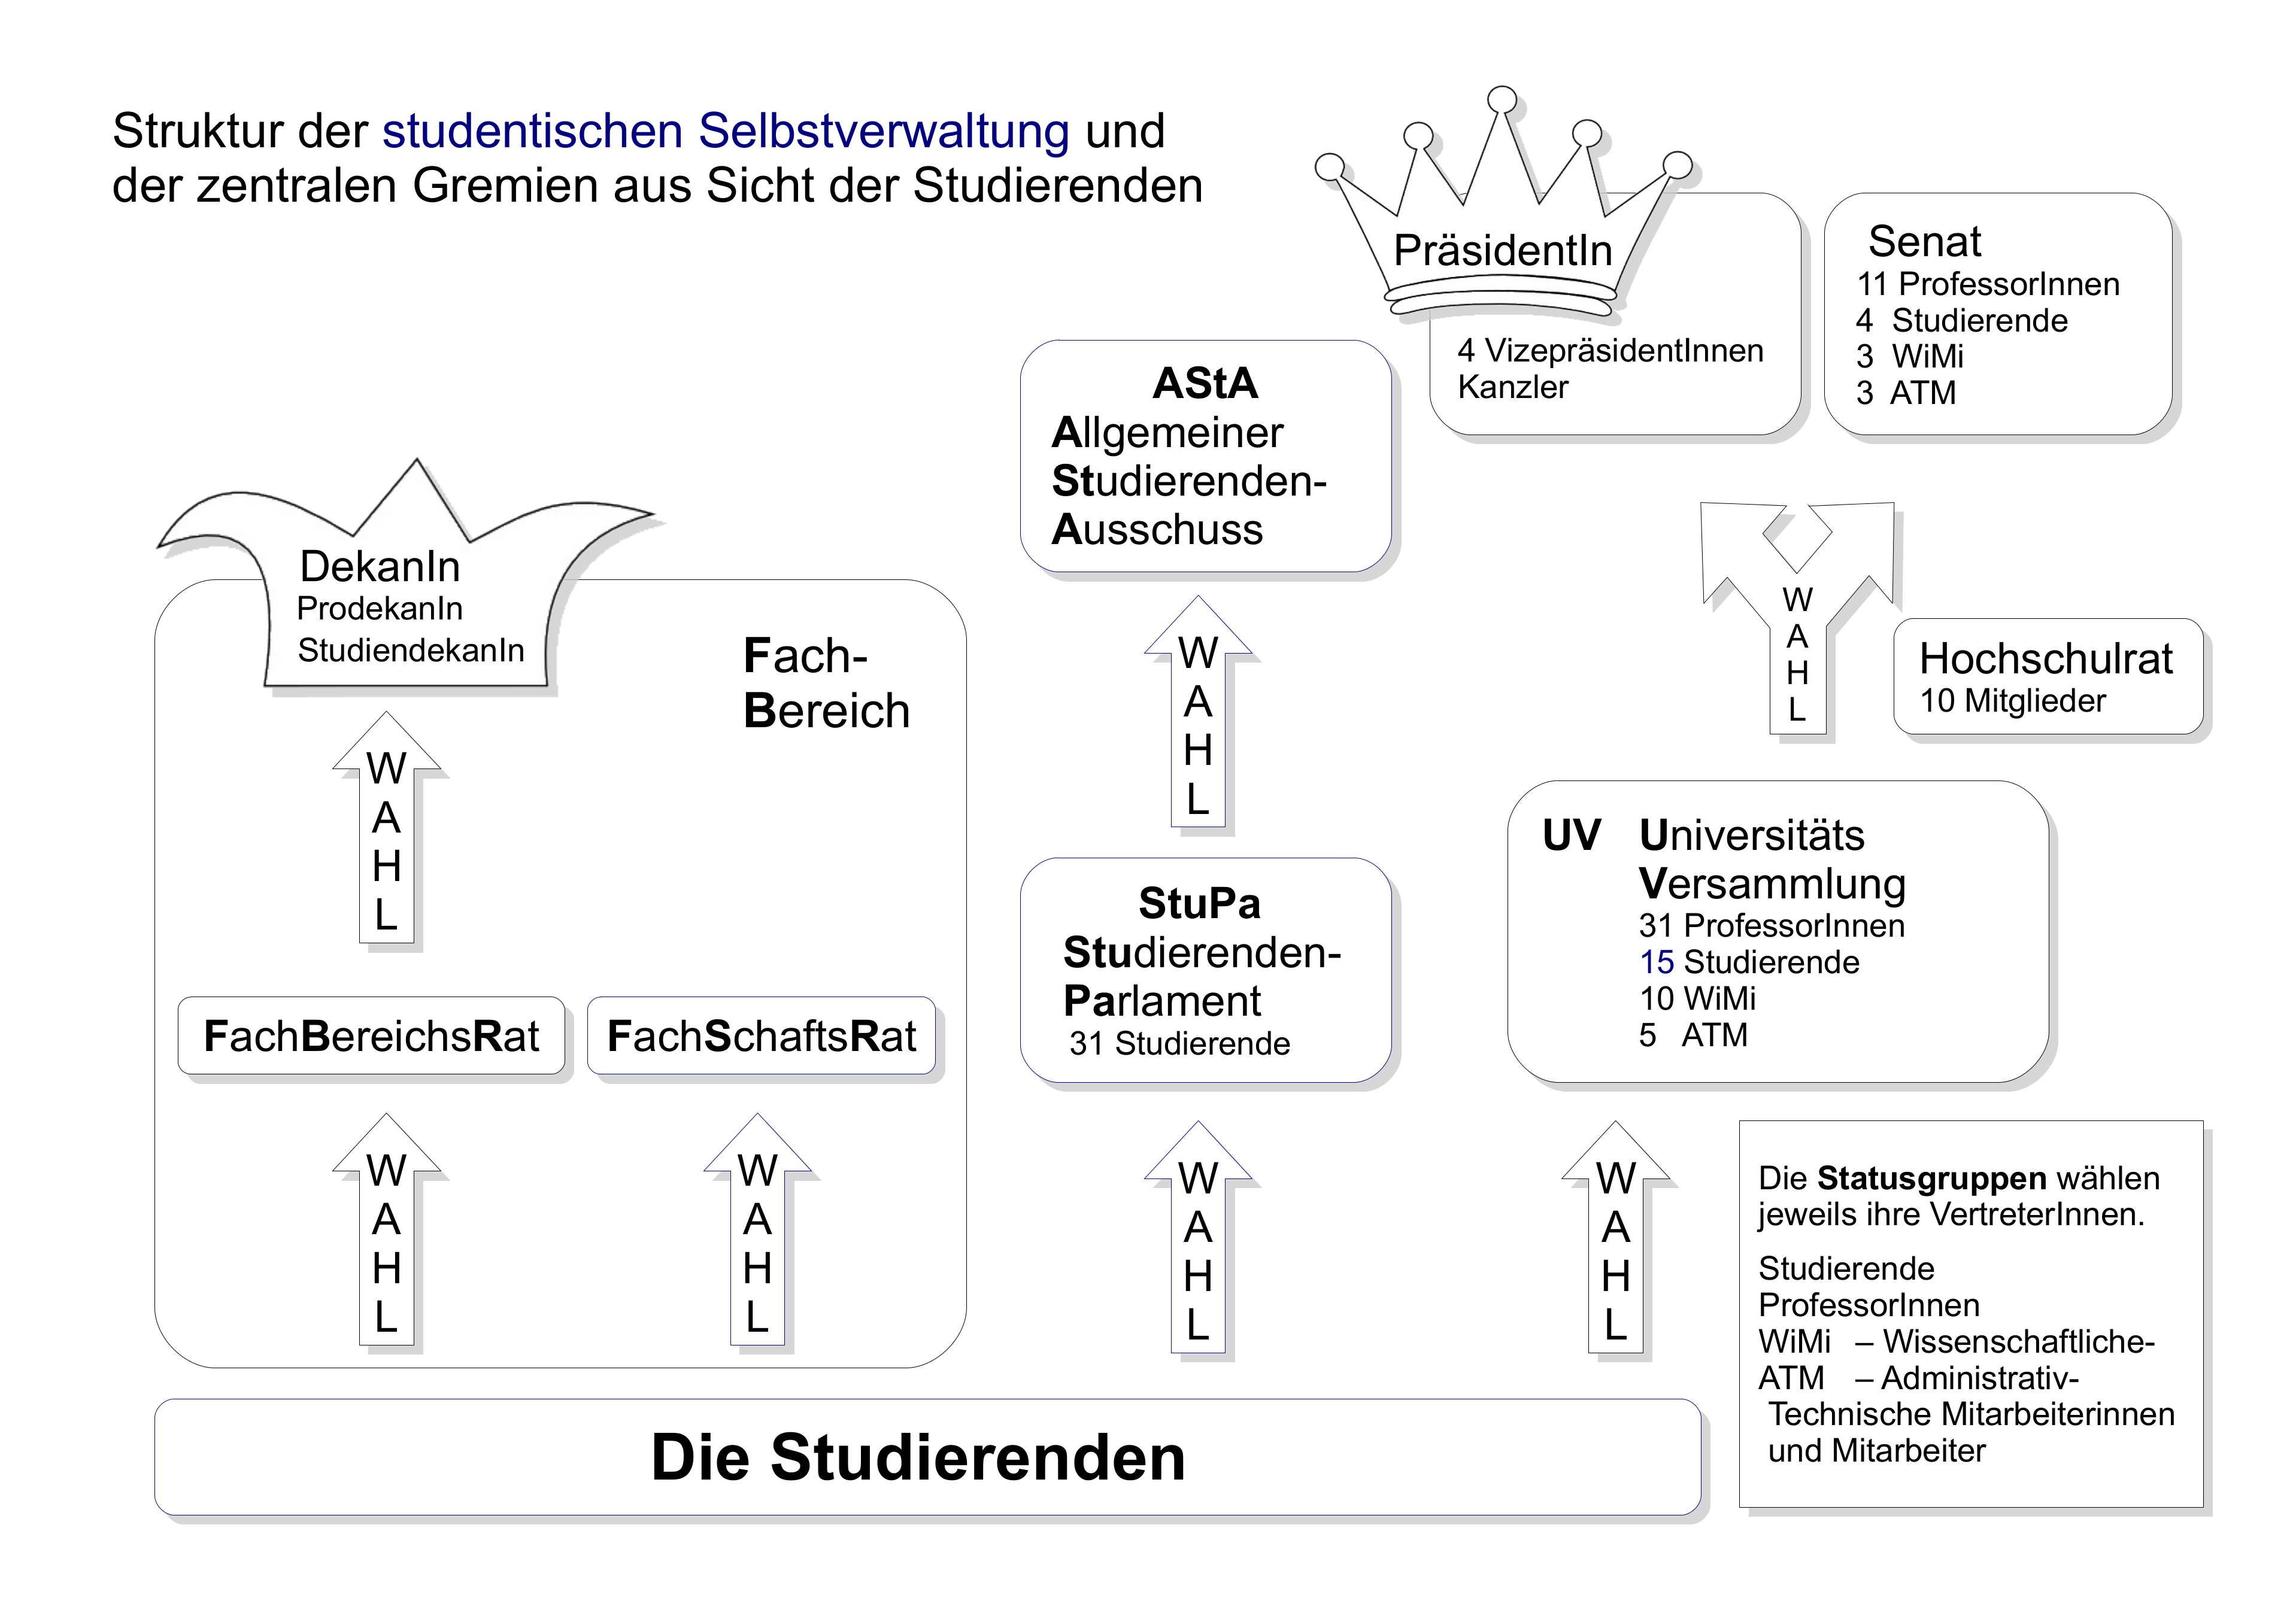
\includegraphics[angle=270,totalheight=17cm]{artikel/hopo2}

\newpage

\artikel{Der AStA der TU Darmstadt}
{Der Allgemeine Studierendenausschuss (AStA) ist die oberste Vertretung aller Studierenden auf Universitätsebene. Darüber hinaus ist er Ansprechpartner bei Problemen und bietet für Studierende etliche Service- und Beratungsangebote.
    Wer der AStA eigentlich ist und was er alles so macht, erfährst du in diesem Artikel.
}{
    \noindent\textbf{Aufgaben des AStA}\\
    Die Aufgaben des AStA sind vielfältig und leiten sich aus den Aufgaben der Studierendenschaft ab, die nach §3 der Satzung der Studierendenschaft definiert sind:

    \begin{itemize}
        \item	Die Vertretung der Gesamtheit ihrer Mitglieder im Rahmen ihrer gesetzlichen Befugnis.
        \item	Die Wahrnehmung der hochschulpolitischen Belange ihrer Mitglieder.
        \item	Die Wahrnehmung der wirtschaftlichen und sozialen Belange der Student*innen. Die Zuständigkeit des Studierendenwerkes (StuWe) oder anderer Träger bleibt unberührt.
        \item	Die Pflege überregionaler und internationaler Studierendenbeziehungen.
        \item	Die Förderung der politischen Bildung und des Verantwortungsbewusstseins von Student*innen für ihre Rolle als Staatsbürger*innen. Hierzu gehört auch die Förderung eines wissenschaftlich fundierten, kritischen Verständnisses der Student*innen von ihrer jetzigen und künftigen Tätigkeit und der Rolle von Wissenschaft und Technik in der Gesellschaft.
        \item	Die Unterstützung kultureller und musischer Interessen der Student*innen.
    \end{itemize}

    Das mag erst einmal alles sehr förmlich und theoretisch klingen, doch tatsächlich arbeiten täglich AStA-Referentinnen und -Referenten daran, die Studienbedingungen an der TU zu verbessern. Der AStA engagiert sich zum Beispiel für Studierende in sozialen Notsituationen und steht im ständigen Kontakt mit der Universitätsleitung. Er sorgt mit seinen Gewerben und Veranstaltungen für mehr Kulturangebote in Darmstadt und ist zum Beispiel auch dafür verantwortlich, dass es das Semesterticket in seiner jetzigen Form überhaupt gibt.
    Du siehst also: Der AStA hat durchaus auch Einfluss auf deinen Studienalltag.\\

    \bildmitunterschrift{artikel/eule_final_orange}{width=\linewidth}{}{}


    \noindent\textbf{Doch wie kommt man eigentlich in den AStA?}\\
    Der AStA besteht größtenteils aus Referenten und Referentinnen, die jedes Jahr vom Studierendenparlament gewählt werden. Neben diesen gewählten Referaten gibt es inzwischen auch viele eingestellte Referate, die von engagierten Studierenden geleitet werden, die mit einem tollen Projekt zum AStA gekommen sind und dann für ihr jeweiliges Referat eingestellt wurden.

    Aktuell gibt es zum Beispiel Referate zum Thema: Nachhaltigkeit, Queer, Feminismus, Mobilität, Inklusion, Familienförderung und noch vieles mehr.\\
    \columnbreak

    \subsection*{Angebote des AStA im Detail}

    Neben dem politischen Engagement ist der AStA wie eingangs schon erwähnt für viele Servicangebote zuständig. Hier eine kleine Auswahl.\\

    \noindent\textbf{Fahrradverleihsystem Call a Bike}\\
    Für alle Darmstädter Studierenden ist beim Leihfahrradsystem "`Call a Bike"' der Deutschen Bahn jeweils die erste Stunde jeder Fahrt kostenlos. Und das auch noch deutschlandweit! Die Räder können ganz einfach an einer Station entliehen und an einer beliebigen anderen Station zurückgegeben werden. In Darmstadt gibt es inzwischen über 30 Stationen und eine liegt direkt am Piloty. Mehr zum Angebot unter \footnotemark[1].\\

    \noindent\textbf{RMV-AStA Semesterticket}\\
    Dein Studienausweis ist gleichzeitig dein Semesterticket und bietet kostenlose Fahrten mit dem öffentlichen Nahverkehr im gesamten RMV-Gebiet und teilweise auch im Übergangsgebiet (siehe Grafik auf der nächsten Seite). Die Konditionen für dieses Ticket verhandelt regelmäßig der AStA und er ist auch dein Ansprechpartner bei allen Fragen um das Ticket (z.B. Ticket-Erstattung bei Auslandssemestern). Mehr unter \footnotemark[2].\\

    \noindent\textbf{AStA-Büros}\\
    Die AStA-Büros in der Stadtmitte (S1$|$03-62) und auf der Lichtwiese (L3$|$01-70) sind deine erste Anlaufstelle, wenn du Fragen zum AStA, den Angeboten oder auch generell zu Geschehnissen in der Universität hast. Auch wenn du dich selbst gerne einbringen würdest oder ein Projekt starten willst, bist du hier richtig. Lagebeschreibung und Öffnungszeiten unter \footnotemark[3].\\

    \noindent\textbf{Beratungsangebote}\\
    Der AStA organisiert und vermittelt kostenlose Erstberatung zu vielen verschieden Themen. Im Detail sind dies derzeit die BAföG- und Sozialberatung, die Rechtsberatung durch erfahrene Anwälte, die Mietrechtsberatung, die Arbeitsrechtsberatung in Zusammenarbeit mit dem DGB und die Sprechstunde für internationale Studierende. Wenn du nicht genau weißt, an welche der vielen Beratungsstellen du dich eigentlich mit deinem Problem wenden sollst, dann frag am Besten einfach mal in einem der AStA-Büros nach. Infos und aktuelle Sprechzeiten findest du unter \footnotemark[4].\\

    \noindent\textbf{Kultur-Kooperationen}\\
    Aus dem Semesterbeitrag gehen 0,50 \euro~ an das Staatstheater Darmstadt. Dafür hat jede*r Studierende die Möglichkeit, kostenlos Restkarten für Theater, Konzerte, Ballett, Opern oder Musicals im Staatstheater zu bekommen. Wie es geht, steht unter \footnotemark[5].\\

    \noindent\textbf{Studentische Gewerbe}\\
    Neben den Serviceangeboten ist der AStA auch zuständig für eine Vielzahl an Gewerben, welche größtenteils von Studierenden verwaltet werden. Direkt auf dem Campus Stadtmitte findet man das Kulturcaf\'e 806qm und die Fahrradwerkstatt 20$^\circ$. Dazu kommen noch der Schlossgarten (der Biergarten auf der Bastion des Schlosses) und der Nachtclub Schlosskeller, der für seine Musik abseits des Mainstream bekannt ist. Auf dem Campus Lichtwiese betreibt der AStA außerdem einen Papierladen.

    Alle weiteren Infos rund um den AStA und dessen weitere Angebote findest du auf der AStA-Homepage unter \footnotemark[6].
}
{Julian Haas}

\footnotetext[1]{\url{https://www.asta.tu-darmstadt.de/asta/de/angebote/call-a-bike}}
\footnotetext[2]{\url{https://www.asta.tu-darmstadt.de/asta/de/angebote/semesterticket}}
\footnotetext[3]{\url{https://www.asta.tu-darmstadt.de/asta/de/angebote/bueros}}
\footnotetext[4]{\url{https://www.asta.tu-darmstadt.de/asta/de/angebote/beratung}}
\footnotetext[5]{\url{https://www.asta.tu-darmstadt.de/asta/de/angebote/staatstheater}}
\footnotetext[6]{\url{https://www.asta.tu-darmstadt.de}}

\newpage

\addsec{Gültigkeitsbereich des Semestertickets}

\vfill
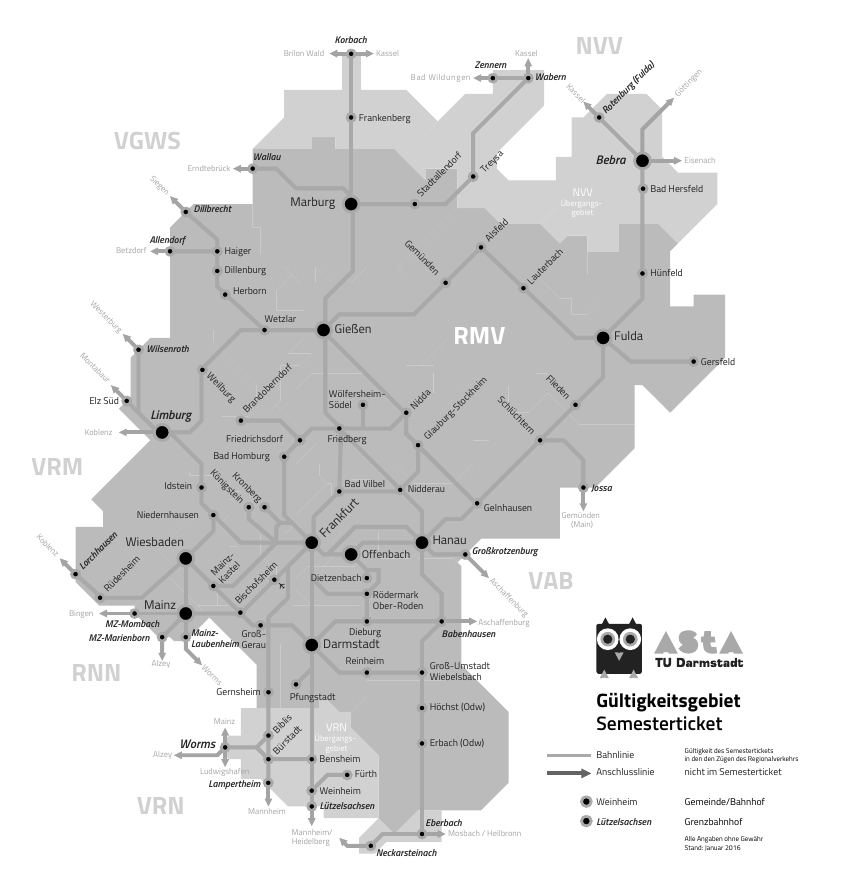
\includegraphics[width=\textwidth+1cm,trim={0.5cm 0cm 1cm 0cm}, clip]{artikel/semesterticket}
\vfill

\newpage


    \kapitel{Freizeit}{../grafik/wesen/wesen_grill_hochzeitsturm}
{Das Semester ist eine unangenehme Unterbrechung der Ferien}
{Johann Jakob Nöggerath (auch Noeggerath), /1788 - 1877), dt. Mineraloge und Geologe, ab 1814 Königlich Preußischer Geheimer Baurat}

\artikel{Leben in Darmstadt}
{Weil Lernen eben nicht alles ist: Auch Studierende sollten sich Freizeit gönnen. Und da man in Darmstadt viel unternehmen kann, findest du hier einige Anregungen.
}{
    Die vorigen Seiten haben sich mit der akademischen Seite des Studiums beschäftigt. Zum Studium gehört aber noch ein anderer, wichtiger Teil: die Freizeit. Sie dient als Ausgleich zu einem anstrengenden Tag und schenkt Erholung, um den nächsten Tag mit neuer Kraft meistern zu können und: sie lenkt uns ab und hilft so, den Kopf wieder frei zu bekommen.

    Deshalb ist es so wichtig, gerade auch in angespannten Wochen auf fest eingeplante Freizeitpausen zu achten. Lernen ist wichtig, aber mit einem freien Kopf geht es deutlich leichter. Ein Praktikum muss fertig werden, die Abgabe steht bevor - wenn du nicht erst am letzten Tag anfängst, musst du nicht bis Mitternacht daran arbeiten.

    Zur guten Freizeitgestaltung gehören gesellige Treffen (Partys, Spielabende usw.) genauso wie sportliche Aktivitäten. Die folgenden Seiten sollen dir dabei helfen, die verschiedenen Möglichkeiten in Darmstadt kennenzulernen und das für dich passende Freizeitprogramm zusammenzustellen.
}
{Tobias Freudenreich, Martin Tschirsich, Stefan Gries}

\artikel{Einfach mal abschalten}
{Eine der angenehmsten Möglichkeiten, seine Freizeit zu verbringen, ist einfach mal abzuschalten und sich zu entspannen, was besonders an wärmeren Tagen an der frischen Luft äußerst angenehm ist.
}{
Darmstädterinnen und Darmstädter finden in ihrer Heimat eine Vielzahl schöner Orte zum Wohlfühlen und Entspannen, welche selbst von älteren Semestern unentdeckt bleiben: Im Norden der Bürgerpark direkt am Nordbad, im Süden an der Heidelberger Straße der Prinz-Emil-Garten und die Orangerie, am Ostbahnhof der Tiergarten Vivarium und die Rosenhöhe.
Den Herrngarten, Darmstadts größte Parkanlage, können Informatikstudierende dagegen nicht übersehen, denn er befindet sich direkt auf der Rückseite des Piloty-Gebäudes. Auch die Mathildenhöhe mit dem Hochzeitsturm als Wahrzeichen Darmstadts und regelmäßigem Kunst- und Kulturprogramm darf nicht unbekannt bleiben.
Im Sommer versprechen Freibäder und Badeseen Abkühlung: Neben den Schwimmbädern der Stadt, über die man sich am besten direkt online informiert, gibt es noch folgende Empfehlungen für Studierende: Das kleine Uni-Freibad direkt neben dem Hochschulstadion, welches durch kostenlosen Eintritt mit Studienausweis und WLAN-Versorgung auf der Liegewiese punkten kann. 
Wer lieber im See badet, der begibt sich kostenlos in das Arheilger Mühlchen oder in die Grube Prinz von Hessen. Beide liegen aber etwas außerhalb, näher an der Uni ist der Große Woog.
}
{Tobias Freudenreich, Martin Tschirsich, Stefan Gries}
\newpage
\artikel{Sport}
{Wie keine andere Freizeitaktivität eignet sich Sport dazu, den Kopf frei zu bekommen und die Kreativität zu fördern: Gesellig ist es allemal, die Sportart sollte allerdings zu den eigenen Bedürfnissen passen.
}{
    Wer wettkampforientiert ist, tendiert eher zu Ball- und Kampfsportarten, wer beim Sport treiben lieber seine Ruhe hat und die Natur genießen möchte, fährt mit dem Rad zur Burg Frankenstein oder geht im Park joggen.
    Insbesondere auch für die Unentschlossenen bietet sich ein Blick in den Katalog des Unisport-Zentrums (USZ) an - die perfekte Anlaufstelle für Aktiv- und Gelegenheitssportler*innen.

    Das Unisport-Zentrum bietet für alle Studierenden und Angestellten rund 250 Sportangebote in 90 Sportarten pro Woche. Von Fitnessveranstaltungen wie Aerobic oder Schwitz-Fit über Ballsportarten wie Badminton und Fußball bis hin zu den außergewöhnlicheren Sportarten wie Einradhockey, Kanupolo, Unterwasser-Rugby oder Quidditch ist fast alles vertreten.
    Das größtenteils kostenlose Hochschulsportangebot wird jedes Semester in einem Programm-Handzettel und im Internet unter der Adresse \footnotemark[1]  veröffentlicht, dort findet sich auch eine Online-Anmeldung für alle Kurse. Das Unisport-Zentrum betreibt zudem eine eigene Golf-Übungsanlage und das Sport- und Gesundheitszentrum, ein Fitnessstudio für Studierende und Angestellte. Neben diesen permanenten Einrichtungen werden zusätzlich noch einzelne Workshops wie Tauchen oder Stepptanz angeboten.
    Am besten gehst du einfach hin und meldest dich kurz nach Semesterbeginn an, lediglich einige spezielle Kurse verlangen zusätzlich die Zahlung einer geringen Gebühr. Das beliebteste Angebot war in den vergangenen Semestern das Uni-Freibad am Hochschulstadion.

    Darüber hinaus führt das studentische Sportreferat in jedem Semester interne Hochschulmeisterschaften (IHM) in verschiedenen Sportarten wie Fußball, Badminton, Tischtennis und Volleyball durch. Wettkampfinteressierte Studierende können außerdem an den Deutschen Hochschulmeisterschaften (DHM) teilnehmen. Die Ausschreibungen und Meldetermine findest du auf den Internetseiten des USZ (IHM) oder unter \footnotemark[2] (DHM).

    Leider sind einige Angebote des USZ überlaufen und eignen sich tatsächlich nur zum Kennenlernen. Hier bietet es sich dann an, einem der lokalen Sportvereine beizutreten. Aus Platzgründen können wir hier keine Übersicht geben, aber eine kurze Suche im Internet führt hier schnell zum Erfolg. Oft bieten diese Vereine für Studierende auch vergünstigte Beiträge an.
    Solltest du bisher noch nicht fündig geworden sein, warten in Darmstadt neben der Eissporthalle und einem Kletterwald am Hochschulstadion noch diverse Parks und weitere Schwimmbäder sowie viele andere Angebote auf dich.
    Dazu kommen Gruppen wie das Juggerteam von Darmstadt, Pink Pain [3], die ganz ohne Verein Sport machen.
}
{Tobias Freudenreich, Martin Tschirsich, Stefan Gries}

\footnotetext[1]{\url{https://online-anmeldung.usz.tu-darmstadt.de/sportarten/aktueller_zeitraum}}
\footnotetext[2]{\url{http://www.adh.de}}
\footnotetext[3]{\url{http://www.jugger-darmstadt.de}}
\newpage


\artikel{Darmstadt kulinarisch}
{Darmstadt bietet einige Essens- und Ausgehmöglichkeiten. Einige davon verstecken sich aber.
}{
\textbf{Frühstücken…}

Besonders während der vorlesungsfreien Zeit möchtest du sicher gerne einmal mit Kommilitoninnen und Kommilitonen gemütlich frühstücken.

Hier bietet sich das Caf\'e Chaos an, bis 24 Uhr wirst du hier mit frischen Brötchen versorgt. Am Marktplatz befinden sich das Caf\'e Extrablatt sowie Bäckerei Bormuth - beide bieten ein reiches Frühstücksbuffet.

Auf der anderen Seite der Universität gibt es noch das 3klang am Riegerplatz mit einem sonntäglichen Buffet der Spitzenklasse.\\
Für einen gemütlichen Kaffee zwischendurch bietet sich außerdem das 221qm (Teil des 806qm) direkt auf dem Unigelände an (Eingang an der Alexanderstraße).
\\\\
\textbf{Einfach nur essen…}

Wer mittags Hunger bekommt, geht meist in die Mensa, denn dort gibt's brauchbares, günstiges Essen. Aber womit den Magen füllen, wenn die Mensa schon geschlossen hat oder du einfach mal Abwechslung von der Mensaspeisekarte brauchst?

In der Stadtmitte hast du eine große Auswahl an Alternativen: Dönerläden, Asia-Imbisse, Fastfood-Ketten - alle kaum zu übersehen. Bei manchen gibt es sogar spezielle Studierendenangebote.

Noch deutlich näher an der Uni sind Havana, Hotzenplotz (nur abends geöffnet) und Hobbit. Alle Kneipen liegen in der Lauteschlägerstraße (östlich vom Kantplatz), wobei es im Hobbit mittags Pizzen günstiger gibt. Hinter dem Mathebau liegt das Petri (nur abends geöffnet) mit Biergarten und bayerischer Küche. Die Auswahl ist nicht sehr groß, dafür ist das Essen gut.

Wer vegetarische/vegane Küche bevorzugt, dem sei das Café Habibi in der Landwehrstraße (direkt am Willy-Brandt-Platz) und das Mondo Daily in der Grafenstraße ans Herz gelegt. Im Habibi gibt es zu studentischen Preisen eine Vielzahl an vegetarischen und veganen Gerichten in schöner Atmosphäre zwischen Darmstädter Altbauten, während man im Mondo Daily ein täglich wechselndes Angebot an orientalischen Gerichten genießen kann.
Beide bieten auch einen günstigen Mittagstisch an.

Zuletzt ein wahrer Geheimtipp für Suppenliebhaber: Suppkult Elisabeth in der Schulstraße.\\

\textbf{Etwas trinken…}

Für ein (oder mehr) Bier am Abend bieten sich Pubs wie das Green Sheep in der Erbacher Straße an. Hier gibt es außerdem von 18 bis 20 Uhr Pizza zum halben Preis.

Wer es weniger "`englisch"' mag, kann das Schlossgartencaf\'e aufsuchen: es befindet sich direkt auf der Bastion am Schloss (über die Brücke und dann gleich rechts).
Ein weiteres Urgestein der Darmstädter Kneipenkultur ist die "`Goldene Krone"'. Hier ist es immer voll, die Stimmung ist immer gut und es gibt neben Musik und verschiedenen Events (fast) die ganze Nacht Getränke zu günstigen Preisen.

Draußen sitzen kann man im Sommer im Biergarten Lichtwiesn direkt bei der Mensa Lichtwiese, sowie im Biergarten Darmstadt in der Dieburger Straße.

Wenn du Bier lieber direkt von der Brauerei trinken möchtest, hast du in Darmstadt große Auswahl: die Grohe-Brauerei an der Nieder-Ramstädter Straße, den Ratskeller am Marktplatz und das Braustüb'l am Hauptbahnhof warten auf deinen Besuch.

Für Cocktail-Liebhaber empfiehlt sich das Enchilada (mexikanisch, Happy Hour bis 20 Uhr und montags Cocktailwürfeln) und das Corroboree (australisch, montags Cocktails für die Hälfte) in der Kasinostraße (Haltestelle Rhein-/Neckarstraße). Außerdem gibt es noch die Havana-Bar in der Lauteschlägerstraße und das Sausalitos (Happy Hour bis 20 Uhr) in der Nähe von S3$|$06.
}
{Tobias Freudenreich, Martin Tschirsich, Stefan Gries,
überarbeitet von Julian Haas}

\newpage

\artikel{Abendprogramm}
{Heute Abend schon was vor?
}{
    \textbf{Kino}

    In Darmstadt gibt es diverse Kinos: das Kinopolis am Bahnhof und die kleineren Kinosäle Helia, Pali, Festival und Rex in der Nähe des Luisenplatzes. Das komplette Programm findest du tagesaktuell unter  \footnotemark[1].
    Als gute Alternative zum normalen Kino gibt es die Vorstellungen des studentischen Filmkreises. In der Regel finden während der Vorlesungszeit jede Woche zwei Filmvorführungen statt. Dazu gibt es vorher jeweils einen Kurzfilm, und außerdem kaum Werbung und vor allem kein Popcornmonopol – Essen und Getränke dürfen selbst mitgebracht werden.

    Eine Karte kostet 2,50\euro. Zusätzlich muss ein Mitgliedsausweis erworben werden, welcher zusammen mit dem Eintritt aber immer noch weniger als ein normaler Kinobesuch kostet und ein Jahr lang gültig ist. Er kann vor jeder Vorstellung direkt an der Kasse gekauft werden. Das aktuelle Programm findest du unter \footnotemark[2].

    Wer es lieber luftig mag, kann im Sommer im Schlosshof das Open-Air-Kino besuchen.\\

    \textbf{Theater}

    Viel Kultur bietet ein Besuch im Staatstheater Darmstadt. Studierende erhalten hier unter Vorlage des Studienausweises einen Rabatt und darüber hinaus ab drei Tage vor Veranstaltungsbeginn die Restkarten, egal welcher Preisklasse, komplett kostenlos. So kann ein Theaterbesuch deutlich günstiger sein als Kino.

    Außerdem gibt es auch das halbNeun-Theater \footnotemark[3] und das Theater Moller Haus \footnotemark[4].
    \\\\
    \textbf{Lyrik}

    Definitiv lohnenswert ist der Besuch eines Poetry Slams. Diese finden monatlich in der "`Goldenen Krone"' statt und teilweise auch in der Centralstation. Wenn du selbst einmal vor Publikum stehen willst, bietet der Krone Slam darüber hinaus auch eine offene Liste für Neulinge.
    Unter \footnotemark[5] und \footnotemark[6] gibt es jeweils aktuelle Termine. Außerdem gibt es in Seeheim noch die Open-Air-Dichterschlacht.
    \\\\
    \textbf{Musik}

    Im Schlosskeller (im Innenhof des Schlosses) gibt es je nach Wochentag verschiedene Musikrichtungen zu hören. Das Angebot ist breit gefächert und oft hört man bisher Ungehörtes. Zusätzlich finden hier in regelmäßigen Abständen Musikevents statt. Einfach mal auf \footnotemark[7] vorbeischauen.
    Im dem Caf\'ebetrieb über Tag gibt es hier abends Konzerte zum Studentenpreis. Das Programm findet man unter \footnotemark[8].
    Sowohl der Schlosskeller als auch das 806qm sind Gewerbe des AStA, sodass Einnahmen in gewissen Teilen wieder der Studierendenschaft zugute kommen.

    Musik und Kabarett gibt es in der Centralstation (im Innenhof des City-Carree). Tickets und Informationen zum aktuellen Programm gibt es unter \footnotemark[9]. Ein ähnliches Angebot gibt es im Darmstädter Kongresszentrum, dem darmstadtium. Wem die Leuchtwerbung über dem Haupteingang nicht auffällt, der kann unter \footnotemark[10] die kommenden Veranstaltungen nachschlagen.

    Freunde klassischer Musik kommen mit den Aufführungen der Philharmonie Merck im regionalen Umfeld sowie den Konzerten im Staatstheater auf ihre Kosten. Zuweilen bieten auch Hochschulgruppen wie das Orchester der TU Darmstadt oder der Chor Kostproben ihres Könnens.\\

    \textbf{Party}

    Wer's lieber laut und tanzbar mag, sollte sich einmal die Clubs in Darmstadt näher ansehen: auch hier ist für praktisch jeden Geschmack etwas vorhanden – neben der Goldenen Krone nahe des Schlosses mit sehr gemischtem Programm, dem oben erwähnten Schlosskeller und der House/Hip-Hop/Dancehall Großraum-Disco Musikpark Darmstadt ("`A5"') in Richtung Weiterstadt gibt es in Mühltal-Traisa (etwas außerhalb von Darmstadt) auch noch das Steinbruch Rock-Theater für Freundinnen und Freunde härterer Musik.
    In der Innenstadt findet ihr außerdem noch das Nova mit verschiedenster Tanzmusik.

    Ansonsten reicht, was Partys angeht, eigentlich fast schon ein Verweis auf \footnotemark[11]: So gut wie alle aktuellen Partys und Veranstaltungen sind hier eingetragen. Ansonsten findest du auch in verschiedenen Kultur-Magazinen, zum Beispiel dem P-Magazin, viele Anregungen zum Abfeiern.

    Ganz groß finden in Darmstadt außerdem jedes Jahr zwei Straßenfeste rund um das Schloss statt: das Heinerfest und das Schloßgrabenfest. Das Schloßgrabenfest zeichnet sich vor allem durch viele Bühnen aus, auf denen verschiedene Musikrichtungen gespielt werden, während das Heinerfest das größte und älteste hessische Volksfest ist.

    Drumherum in den Darmstädter Stadtteilen finden ebenfalls (wenngleich kleinere) Straßenfeste statt und die Pfalz ist mit ihren vielen Weinfesten im Spätsommer auch nicht weit. \\
    \\\\
    \textbf{Angebote der Fachschaft}

    Games no Machines (GnoM) ist der Spieleabend der Fachschaft Informatik. Hier kannst du gemütlich mit Kommiliton*innen zusammensitzen und alle erdenklichen Gesellschaftsspiele ausprobieren, genießen, perfektionieren oder wonach dir auch immer der Sinn steht. Mehr hierzu findest du im entsprechenden Artikel.\\
    Während es bei GnoM um Gesellschaftsspiele geht, geht es bei seinem kleinen Bruder, dem RPGnoM, um Pen-and-Paper Rollenspiele.
    Der RPGnoM ist der offene Rollenspielabend der Fachschaft und findet ca. ein Mal pro Monat statt. Er richtet sich an alle, egal ob erfahrene*r Rollenspieler*in oder Neuling. Neben Rollenspielrunden mit diversen Systemen gibt es regelmäßig auch Diskussionsrunden und Workshops rund um das Hobby. Alle Infos und Termine erhaltet ihr auf der Mailingliste unter \footnotemark[12].

    Die Games-Gruppe trifft sich während der Vorlesungszeit, um allen Hobby-Spiele\-ent\-wicklern und Interessierten eine Austauschsplattform zu bieten und in kleineren Gruppen Spiele zu entwickeln. Auch hier gilt, bei Interesse kann man sich an \mbox{games@D120.de} wenden.

    Du möchtest auch so eine Gruppe leiten und hast eine tolle Idee dafür (z.B. Schachabend, Debattierclub, Münzfußball)? Melde dich einfach in D120. Wir helfen dir, dein Projekt bekannt zu machen und Räume dafür zu finden.
}
{Tobias Freudenreich, Martin Tschirsich, Stefan Gries,
    überarbeitet von Julian Haas, Johannes Alef}

\footnotetext[1]{\url{http://www.kinos-darmstadt.de}}
\footnotetext[2]{\url{https://www.filmkreis.de}}
\footnotetext[3]{\url{http://www.halbneuntheater.de}}
\footnotetext[4]{\url{http://www.theatermollerhaus.de}}
\footnotetext[5]{\url{http://krone-slam.de}}
\footnotetext[6]{\url{https://www.facebook.com/Dichterschlacht}}
\footnotetext[7]{\url{https://www.schlosskeller-darmstadt.de}}
\footnotetext[8]{\url{https://www.806qm.de}}
\footnotetext[9]{\url{http://www.centralstation-darmstadt.de}}
\footnotetext[10]{\url{https://www.darmstadtium.de}}
\footnotetext[11]{\url{http://www.partyamt.de}}
\footnotetext[12]{\url{https://lists.d120.de/mailman/listinfo/rpgnom}}

\newpage

\artikel{GnoM - Die LAN-Party ohne Strom}
{Reise mit der Fachschaft Informatik durch die Zeit und entdecke längst vergessene Traditionen wieder.
}{
    Wenn selbst die eingefleischtesten Informatiker*innen abends ihre Kaffeetassen vom Computerpool in überirdische Räume bewegen, dann muss dort schon etwas ganz besonderes geboten werden. In Scharen wandern sie zum Raum E202, beladen mit Süßigkeiten und mysteriösen Kisten ohne USB-Anschlüsse und Netzteile. Außenstehende mögen sich nun vielleicht fragen, was Informatikstudierende mit so einer Kiste anfangen wollen. Die Antwort ist einfach: Die wollen doch nur spielen.
    Am Raum E202 angekommen sieht man auch Mathematik- und Physikstudierende ins Piloty-Gebäude strömen. Manche Langzeitstudent*innen fühlen sich zurückversetzt in ihre Jugendzeit vor der Erfindung der Elektrizität und sind schon versucht, eine Kerze anzuzünden, doch das ist nicht nötig, denn das Anti-Strom-Gebot erstreckt sich nur auf die Unterhaltungsmedien. Hier ist das Motto "`Games no Machines"' (kurz GnoM) Programm.
    Bei diesem legendären Spieleabend der Fachschaft Informatik werden schon seit $10101_2$ Jahren die guten alten Brett- und Kartenspiele hervorgekramt und die PCs im Pool gelassen.
    Alle Informatik-, Physik- und Mathematikstudierenden und auch andere Lebensformen sind herzlich eingeladen, sich selbst davon zu überzeugen, wie viel Spaß eine LAN-Party ohne Strom machen kann. Eigene Spiele dürfen dabei auch gerne mitgebracht werden.\\
    Die erste Möglichkeit, diese ungewöhnliche Erfahrung zu machen, hast du übrigens am Freitag der Ophase in C301, dem Raum über dem Bistro Athene.\\
    Mehr zu den Terminen gibt es über die GnoM-Mailingliste \footnotemark[1], im Fachschaftsblog "`das Wesentliche"' \footnotemark[2] und sonst überall, wo sich hilfsbereite Fachschaftler*innen aufhalten. Generelle Infos findet man zudem auch unter \footnotemark[3].
}
{Alexandra Weber,\\
    überarbeitet von Julian Haas}

\footnotetext[1]{\url{http://www.d120.de/mailman/listinfo/gnom}}
\footnotetext[2]{\url{http://daswesentliche.d120.de}}
\footnotetext[3]{\url{http://www.d120.de/gnom}}

\vfill
\bildmitunterschrift{comics/nerd_sniping}{width=\textwidth}{}{xkcd.org}
\newpage


    \null\newpage
    \kapitel{Zum Nachschlagen}{}
{Wer nicht weiß, wie es geht, sollte wissen, wo es steht.}{Arne Pottharst, ehemaliger Fachschaftler}

\addsec{Lesezeichen für Informatikstudierende}

\bigskipamount 7mm

\lesezeichenl{Homepage der TU Darmstadt}{https://www.tu-darmstadt.de}
\lesezeichenr{Fachbereich Informatik}{https://www.informatik.tu-darmstadt.de}
\lesezeichenl{Fachschaft Informatik}{https://D120.de}
\lesezeichenr{Forum der Fachschaft}{https://www.fachschaft.informatik.tu-darmstadt.de/forum}
\bigskip
\lesezeichenl{Infrastruktur und stud. Poolservice des Fachbereichs Informatik (ISP)}{https://www.isp.informatik.tu-darmstadt.de}
\lesezeichenr{ISP-Wiki}{https://support.rbg.informatik.tu-darmstadt.de/wiki}
\lesezeichenl{TUCaN und Vorlesungsverzeichnis}{https://www.tucan.tu-darmstadt.de}
\lesezeichenr{Hochschulrechenzentrum (HRZ)}{https://www.hrz.tu-darmstadt.de}
\lesezeichenl{Athene-Karte}{https://www.hrz.tu-darmstadt.de/id/athenekarte_neu}
\lesezeichenr{Universitäts- und Landesbibliothek}{https://www.ulb.tu-darmstadt.de}
\lesezeichenl{Sprachenzentrum}{https://www.spz.tu-darmstadt.de}
\lesezeichenr{Studierendenwerk Darmstadt}{http://studierendenwerkdarmstadt.de}
\lesezeichenl{AStA}{https://www.asta.tu-darmstadt.de}
\lesezeichenr{Unikalender}{https://www.tu-darmstadt.de/vorbeischauen/kalender}
\bigskip
\lesezeichenl{Hochschulgruppen der TU Darmstadt}{www.tu-darmstadt.de/studieren/campusleben/engagement_student/hochschulgruppen.de.jsp}
\bigskip
\lesezeichenr{Chaostreff Darmstadt}{https://chaos-darmstadt.de}
\lesezeichenl{806qm}{https://806qm.de}
\lesezeichenr{Schlosskeller}{https://www.schlosskeller-darmstadt.de}
\lesezeichenl{Studentischer Filmkreis}{https://www.filmkreis.tu-darmstadt.de}
\lesezeichenr{Kinopolis und CityDome}{https://www.kinos-darmstadt.de}
\lesezeichenl{Veranstaltungskalender für Darmstadt}{https://www.partyamt.de}

\newpage

\addsec{Häufige Abkürzungen}

\textbf{Erläuterungen zu einigen beliebten und gebräuchlichen Abkürzungen an der TU Darmstadt. Für alle, die viele wichtige Sachen noch mal nachschlagen möchten.}

\begin{longtable}{p{20mm}p{85mm}}
APB		&	Allgemeine Prüfungsbestimmungen sind das Regelwerk, nach denen du deine Prüfungen schreiben darfst und musst.\\
AStA	&	Der Allgemeine Studierendenausschuss wird vom Studierendenparlament gewählt und hat verschiedene Referate (Soziales, Fachschaften, Ausländer, uvm.). Er macht Hochschulpolitik und ist zuständig für viele Serviceangebote und Gewerbe wie z.B. den Schlosskeller.\\
B.Sc.	&	Bachelor of Science. Mittlerweile der erste Hochschulabschluss.\\
CE		&	Computational Engineering. Ein Studiengang aus Informatik, Mathematik, Maschinenbau und Elektrotechnik.\\
c.t.	&	cum tempore. Die berühmte akademische Viertelstunde, die man zu spät kommen darf. An der TU Darmstadt gilt aber meist s.t.\\
EH		&	Evangelische Hochschule Darmstadt.\\
ESG		&	Die Evangelische Studierendengemeinde bietet Kurse und Freizeitaktivitäten nicht nur für die Protestanten hier an der TU Darmstadt an und unterhält ein eigenes Studierendenwohnheim.\\
FB		&	Diese Abkürzung steht für Fachbereich. Es gibt 13 verschiedene Fachbereiche an der TU Darmstadt. Jedem Fachbereich ist hierbei eine Nummer zugeordnet. So bekommst du vom FB 4, der Mathematik, deine Mathematikvorlesung. Die Informatik hat die höchste Zahl (FB 20).\\
FBR		&	Im Fachbereichsrat bestimmen Professor*innen, Mitarbeiter*innen und Studierende über Entscheidungen sowie Orientierung des Fachbereichs.\\
FIfF	&	Forum InformatikerInnen für Frieden und gesellschaftliche Verantwortung e.V.\\
FS		&	Die Fachschaft wird meist mit den Studierenden gleichgesetzt, die sich am Fachbereich in irgendeiner Weise engagieren. Formal gehören zur Fachschaft jedoch alle Studierenden eines Fachbereichs.\\
FSK		&	Die Fachschaftenkonferenz trifft sich einmal im Monat, um über fachbereichsübergreifende Themen zu diskutieren und zu entscheiden.\\
FSR		&	Der Fachschaftsrat ist das von dir gewählte Organ der Fachschaft. Er tagt regelmäßig Mittwoch um 18 Uhr in D120 im Robert-Piloty-Gebäude.\\
GnoM	&	Games no Machines ist der Name des Spieleabends der Fachschaft Informatik ohne Computerspiele.\\
h\_da	&	Hochschule Darmstadt, früher Fachhochschule Darmstadt.\\
HDA		&	Die Hochschuldidaktische Arbeitsstelle bringt studentischen Tutor*innen pädagogisches Handwerkszeug bei und berät auch bei Referaten, Bachelor- und Masterarbeiten. Unser Feedback (Evaluation der Lehrveranstaltungen) machen wir mit der HDA zusammen.\\
HRZ		&	Das Hochschulrechenzentrum versorgt die Nichtinformatikerinnen und Nichtinformatiker mit Rechenpower und alle Angehörigen der TU mit WLAN. Es verwaltet die Athene-Karte und bindet die TU Darmstadt an das Internet an.\\
iST		&	Studiengang Informationssystemtechnik, welcher aus Teilen der Informatik und Elektrotechnik besteht.\\
ISP		&	Der neue Name der RBG. ISP steht für Infrastruktur und studentischer Poolservice.\\
KIF		&	Die Konferenz der Informatikfachschaften aus dem deutschsprachigen Raum findet einmal pro Semester statt.\\
KHG		&	Die Katholische Hochschulgemeinde unterhält ein Studierendenwohnheim und organisiert Seminare.\\
LiWi/LW	&	Lichtwiese. Auf der Lichtwiese haben wir Informatikstudierenden selten etwas zu tun. Im Sommer kann man hier draußen im Biergarten sitzen, lernen und entspannen.\\
LZM		&	Im Lernzentrum Mathematik gibt es Skripte, Übungen, alte Klausuren mit Musterlösung und Beratung.\\
M.Sc.	&	Master of Science. Ist gleichwertig zum Diplom und berechtigt auch zur Promotion.\\
Piloty	&	Robert-Piloty-Gebäude (Gebäude S2$|$02) = Hauptquartier und Lebensraum der Informatikerinnen und Informatiker. Man beachte den guten Schutz vor Sonneneinstrahlung, 1A-Anzahl von Poolrechnern, sowie die exzellente Kaffeeversorgung.\\
PO		&	Die Prüfungsordnung regelt die Inhalte des Studiums, die Studienziele und vieles mehr.\\
RBG		&	Die Rechnerbetriebsgruppe ist für die technische Infrastruktur im Fachbereich Informatik verantwortlich. Anfang 2014 wurde sie in ISP umbenannt.\\
RMV		&	Rhein-Main-Verkehrsverbund\\
SFK		&	Der Studentische Filmkreis ist eine Hochschulgruppe, welche zweimal in der Woche Filme im Audimax vorführt.\\
SS n/SoSe n&Das Sommersemester des Jahres n\\
s.t.	&	sine tempore. Ohne akademische Viertelstunde muss man pünktlich kommen. Gegenteil von c.t.\\
StuPa	&	Studierendenparlament\\
TUCaN	&	TU-Campus-Net\\
TUD		&	Technische Universität Dresden\\
TU Darmstadt&Technische Universität Darmstadt\\
ULB		&	Universitäts- und Landesbibliothek Darmstadt. Der Neubau befindet sich zwischen Mensa und altem Hauptgebäude.\\
USZ		&	Das Unisportzentrum ist am Campus Hochschulstadion zu finden. Hier kann man sich für die meist kostenlosen Angebote anmelden oder Karten dafür erwerben.\\
WInfe	&	Wirtschaftsinformatikerinnen und -informatiker gehören dem FB 1 an.\\
WS m/n	&	Das Wintersemester von Herbst m bis Frühjahr n.\\
ZSB		&	Zentrale Studienberatung. Hilft bei nicht fachspezifischen Studienfragen.\\
\end{longtable}

\newpage

\addsec{Wichtige Adressen}

\textbf{Auf dieser Seite findest du die Adressen einiger wichtiger Einrichtungen. Die Vorwahl von Darmstadt (0 61 51) ist weggelassen.}

\begin{multicols}{2}

    \textbf{Fachschaft Informatik}\\
    S2$|$02 D120\\
    Hochschulstraße 10\\
    64289 Darmstadt\\
    Tel: 16-25522\\
    \url{www.D120.de}

    \vspace{3mm}
    \textbf{Mentorensystem der Informatik}\\
    Kai Kucharzewski\\
    S2$|$02 D009\\
    Hochschulstraße 10\\
    Tel: 16-25520\\
    \href{mailto:mentorensystem@informatik.tu-darmstadt.de}{mentorensystem@informatik.tu-darmstadt.de}

    \vspace{3mm}
    \textbf{AStA TU Darmstadt}\\
    Büro Stadtmitte:\\
    S1$|$03 62\\
    Hochschulstraße 1\\
    Büro Lichtwiese:\\
    L3$|$01 70\\
    Tel: 16-28360\\
    \url{https://www.asta.tu-darmstadt.de}

    \vspace{3mm}
    \textbf{Beauftragter für Behindertenfragen}\\
    Gerhard Schmitt\\
    S1$|$01 211\\
    \href{mailto:schmitt@pvw.tu-darmstadt.de}{schmitt@pvw.tu-darmstadt.de}

    \vspace{3mm}
    \textbf{Hochschulrechenzentrum}\\
    S1$|$22 101\\
    Tel: 16-71112\\
    \url{https://www.hrz.tu-darmstadt.de}


    %Das Leerzeichen soll verhindern, dass LaTeX "Fachstudienberatung Informatik" noch unten in die rechte Spalte setzte, aber die Adresse dann oben in die linke Spalte.
    \

    \vspace{3mm}
    \textbf{Fachstudienberatung Informatik}\\
    S2$|$02 D115\\
    Tel: 16-25518 \\
    \href{mailto:beratung@informatik.tu-darmstadt.de}{beratung@informatik.tu-darmstadt.de}

    \vspace{3mm}
    \textbf{Prüfungssekretariat}\\
    Sabine Haschka\\
    S2$|$02 D117\\
    Tel: 16-25506\\
    Sprechstunde: Di, Mi, Do von 9 bis 12 Uhr

    \vspace{3mm}
    \textbf{Universitätssportzentrum}\\
    Lichtwiesenweg 3\\
    Tel: 16-76555\\
    \url{https://www.usz.tu-darmstadt.de}

    \vspace{3mm}
    \textbf{Studierendenservice}\\
    S1$|$01\\
    Karolinenplatz 5\\
    Tel: 16-26999

    \vspace{3mm}
    \textbf{Amt für Ausbildungsförderung (BAföG)}\\
    Alarich-Weiss-Str. 3 \\
    Tel: 16-29958\\
    \url{http://www.studierendenwerkdarmstadt.de/index.php/de/studienfinanzierung}

    \vspace{3mm}
    \textbf{Universitäts- und Landesbibliothek}\\
    Magdalenenstraße 8\\
    Tel: 16-76211\\
    \url{https://www.ulb.tu-darmstadt.de}

    \vspace{3mm}
    \textbf{Studierendenwerk Darmstadt}\\
    Alexanderstraße 4 \\
    Tel: 16-29811, 16-29813\\
    \url{http://studierendenwerkdarmstadt.de}


\end{multicols}

\newpage



    % Impressum
    \addsec{Impressum}
\small

\textbf{Inforz zur \ophase} – Sonderausgabe der Zeitschrift der Studierenden des Fachbereiches Informatik der Technischen Universität Darmstadt zur \ophase.

\vspace{3mm}
Die Redaktion tagt derzeit unregelmäßig. Die Termine werden über die offene Mailingliste inforz-helfer@d120.de bekannt gegeben. Das Inforz ist im Web unter \url{www.d120.de/inforz/} verfügbar. Interessierte Mitarbeiter*innen sind immer willkommen; siehe \url{www.D120.de/de/studierende/inforz/mitmachen/}.

\vspace{3mm}
Namentlich gekennzeichnete und anonyme Beiträge geben nicht notwendigerweise die Meinung der Redaktion wieder. Alle Rechte, insbesondere das der Verfilmung, vorbehalten.

\bildmitunterschrift{../grafik/wesen/wesen_inforz}{width=3cm}{}{}

\textbf{Redaktionsanschrift:} Inforz, Fachschaft Informatik, Hochschulstraße 10, 64289 Darmstadt\\
\textbf{Webseite:} \url{www.D120.de/inforz/}\\
\textbf{E-Mail:} inforz@D120.de

\vspace{3mm}
\textbf{Redaktionsschluss dieser Ausgabe:} 01. April 2020\\
\textbf{Drucklegung dieser Ausgabe:} 01. April 2020\\
\textbf{V.i.S.d.P.:} Fabian Damken, Fachschaft Informatik, Hochschulstraße 10, 64289 Darmstadt

\vspace{3mm}
\textbf{Redaktion:} Stefan Gries, Jannis Blüml, Nadja Geisler, Julian Haas, Tobias Otterbein, Stefan Pilot, Dorothea Treitz, Fabian Damken

\vspace{3mm}
\textbf{Satz:} Dorothea Treitz mit \LaTeX, unter Verwendung einer Vorlage von Tobias Otterbein\\
\textbf{Bild- und Grafikredaktion:} Claudius Kleemann, Nico Haase, Stefan Pilot, Sven Amann, Tobias Otterbein, Stefanie Blümer, Fabian Damken, Jennifer Nicola

\vspace{3mm}
\textbf{Vielen Dank an:} Jennifer Nicola, Frederik Alexander Bark, Frederik de Vries für die Leitung der \ophase \  sowie an alle weiteren Mitarbeiter*innen und Helfer*innen, auf deren Ideen und Texten dieses Heft aufgebaut ist und die bei der Ophase mitgemacht haben. Vielen Dank an Randall Munroe sowie an Felix Reidl und Fernando Sánchez Villaamil für die tollen Grafiken.\\

\vspace{3mm}
%\textbf{Titelbild:} Fabian Damken\\
\textbf{Rückumschlag:} Tobias Otterbein\\
\textbf{Comics:} \url{www.xkcd.org}, \url{moomug.com} jeweils Creative Commons BY-NC

\vspace{3mm}
\textbf{Druck:} typographics GmbH, Röntgenstraße 27a, 64291 Darmstadt, Deutschland \\
\textbf{Auflage:} 1000 Exemplare \\
\textbf{ISSN:} 1614–4295

\newpage


    % Rückseite
    \thispagestyle{empty}
\ThisCenterWallPaper{0.9}{../grafik/lageplan_mit_markierungen}

\begin{textblock*}{10cm}(7mm,6mm)
    \normalsize \textbf{Dieses Inforz gehört:}
\end{textblock*}

\begin{textblock*}{4cm}(10cm,1cm)
    
\includegraphics[width=4cm]{../grafik/wesen/wesen_uni}
\end{textblock*}


\end{document}
